% % Deeplearn-GAN

% \documentclass[UTF8]{ctexbook}

% \ctexset{
%     part/number = \chinese{part}
% }
% \usepackage{multirow}
% \usepackage{amsmath}% ams 数学公式
% \usepackage{amsfonts}% ams 数学字体
% \usepackage{bbm}%重影字体
% \usepackage{amssymb,latexsym}% ams 数学符号与LaTeX数学符号
% \usepackage{mathrsfs}% 花式符号
% \usepackage{ntheorem}%定理、定义、证明
%     \theoremstyle{nonumberplain}
%     \theoremheaderfont{\bfseries}
%     \theorembodyfont{\normalfont}
%     \theoremsymbol{$\square$}
%     \newtheorem{Proof}{\hskip 2em 证明}
%     \newtheorem{theorem}{\hspace{2em}定理}[chapter]
%     \newtheorem{definition}{\hspace{2em}定义}[chapter] % 如果没有章, 只有节, 把上面的[chapter]改成[section]
%     \newtheorem{axiom}[definition]{\hspace{2em}公理}
%     \newtheorem{lemma}[definition]{\hspace{2em}引理}
%     \newtheorem{proposition}[definition]{\hspace{2em}命题}
%     \newtheorem{corollary}[definition]{\hspace{2em}推论}
%     \newtheorem{remark}{\hspace{2em}注}[chapter] %类似地定义其他“题头”. 这里“注”的编号与定义、定理等是分开的
%     \newtheorem{Assumption}{\hspace{2em}假设}[chapter]

% %算法伪代码
% %http://blog.csdn.net/lwb102063/article/details/53046265
% \usepackage{algorithm}
% \usepackage{algorithmicx}
% \usepackage{algpseudocode}
%     \floatname{algorithm}{算法}
%     \renewcommand{\algorithmicrequire}{\textbf{输入:}}
%     \renewcommand{\algorithmicensure}{\textbf{输出:}}
% % 罗马数字:示例:\rom{2}
% \makeatletter
% \newcommand*{\rom}[1]{\expandafter\@slowromancap\romannumeral #1@}
% \makeatother

% \usepackage{enumerate}%itemiz环境。\begin{enumerate}[step 1][a)]可以使用 A,a,I,i,1 作为可选项产生 \Alph,\alph,\Roman,\roman,\arabic 的效果
% \usepackage{cite}%参考文献
%     \bibliographystyle{plain}
% \usepackage{extarrows}% 带参数的箭头
% \usepackage{hyperref}% 超链接
% \usepackage{pifont}%然后在正文输入\ding{172}~\ding{211}得到相应数字,要是要①就输入:\ding{172}②就输:\ding{173}
% %\usepackage[CJKbookmarks, colorlinks, bookmarksnumbered=true,pdfstartview=FitH,linkcolor=black,citecolor=black]{hyperref}%超链接的格式设置
% \hypersetup{
%     colorlinks=false,% 去掉超链接颜色
%     pdfborder=0 0 0% 取消超链接的边框
% }
% \usepackage{graphicx}% 图片管理
% \usepackage{caption}
% \usepackage{subcaption}%并排的图各有标题
% \graphicspath{{images/}}% 设置图片搜索路径
% \usepackage{float,varwidth}% 浮动体
% \usepackage{booktabs}% 三线表
% \usepackage{fancyhdr}% 页眉设置
% \usepackage{xcolor}% 颜色宏包
% \usepackage{colortbl}% 彩色表格
% \usepackage{listings}% 代码高亮
% \usepackage{caption}% 对标题进行控制,如让\caption标题的字体缩小一号,同时数字标签使用粗体可以用:\usepackage[font=small,labelfont=bf]{caption}
% \usepackage{xfrac,upgreek}%分别是行间公式如a/b的形式(将原来的命令\frac改成\sfrac)和希腊字体的宏包的
% \usepackage{mathtools}%lgathered和rgathered环境把公式向左向右对齐
% \usepackage{tabularx}%提供自动延伸的表列,(X列格式说明符),文字过长时可以自动转行
% \usepackage{longtable}%长表格
% \usepackage{enumitem}%enumerate宏包的升级
% \usepackage{harpoon}%数学公式的矢量
% \usepackage{bookmark}%目录的书签
% \renewcommand{\headwidth}{\textwidth}%图片并排,这个要列在所有宏包的后面
% \definecolor{codegreen}{rgb}{0,0.6,0}
% \definecolor{codegray}{rgb}{0.5,0.5,0.5}
% \definecolor{codepurple}{rgb}{0.58,0,0.82}
% \definecolor{backcolour}{rgb}{0.95,0.95,0.92}
% \lstset{
%     commentstyle=\color{codegreen},
%     keywordstyle=\color{magenta},
%     numberstyle=\tiny\color{codegray},
%     stringstyle=\color{codepurple},
%     basicstyle=\footnotesize,
%     breakatwhitespace=false,% 断行只在空格处
%     breaklines=true,% 自动断行
%     captionpos=b,% 标题位置
%     keepspaces=true,
%     numbers=left,
%     numbersep=5pt,
%     showspaces=false,
%     showstringspaces=false,
%     showtabs=false,% 显示
%     tabsize=2% TAB 被当作两个空格
% }
% \topmargin=0pt\oddsidemargin=0pt\evensidemargin=0pt
% \textwidth=16.5cm\textheight=23cm\raggedbottom%我这么设置是为了缩小页边距,满足有的文字无法转行
% \pagestyle{headings}%页眉为章节标题,无页脚
% \setlength{\abovecaptionskip}{10pt}
% \setlength{\belowcaptionskip}{-15pt}%图片表格的前后距离设置
% \CTEXsetup[format={\zihao{-3}\raggedright\bfseries}]{section}%设置节的格式节的格式


% \begin{document}
\section{对抗生成网络GAN}
    \subsection{引言}
        \par
        对于生成模型而言,我们的任务是拟合(估计)样本分布,并从分布中生成/采样样本。假设你已经有了GAN的思想:用生成器G生成假样本,将假样本和真样本送进判别器D中进行真假判别。判别器D的目标是使假样本被判别为真的概率尽可能小,真样本被判别为真的概率尽可能大;生成器G的目标是使假样本为真的概率尽可能大。判别器D和生成器G交替进行训练,每训练1步G要训练$k$步D。
        \par
        现在,我们来考虑这样的生成器G(generator):
        \begin{enumerate}
        \item 是否需要训练判别器?我们可以将判别器的判别水平提前固定,只有生成器生成的图片/样本能骗过判别器即可。就像一个学生和一个美术老师一样,老师要求学生画一个狮子,而学生从未见过狮子,于是他随便画了个,交给老师,老师说这个不是,狮子尾巴有个球,哪哪哪要改(学生见过其它动物,未见过狮子,并且老师也有一定的知识,老师可以说狮子和……很像),于是学生回去改,再交再改直到老师/判别器满意为止。
        \item 判别器和生成器时训练。我们先将判别器训练到一定的水平,然后再开始生成样本,判别器的目标是使生成样本属于已有样本的概率最小(即在生成器固定的情况下,使概率最小),生成器的目标是使概率最大。老师会通过学生提交的作品提高自己的要求/判别率(无论生成器给出一个什么样的样本,我都要给它判成假的,如果判别效果不好,我就去修改判别器。生成器要让最好的判别效果最差)。
        \item 多个判别器。我们设定多个判别器作为老师(判别器判别率固定也可,渐渐提高也可),然后让生成器去生成样本,要让多个导师都认可才可以。这是一个什么问题?生成器是样本分布的拟和吗?
        \end{enumerate}
        \par
        设有生成器G产生的样本分布函数为$P_g$,密度函数为$p_g$,假样本为$x\sim P_g$;真实样本分布函数为$P_r$,密度函数为$p_r$,真样本为$x\sim P_r$。我们现在是从$P_g$中采样一个$x$,并于真实样本进行判别,即将$P_g$产生的$x$和$P_r$产生的$x$输入到判别器中进行判别。如果判别器D不能辨识真伪,我们就说在D下,$P_g$是$P_r$的估计。
        \par
        我们知道,一般的生成器G是一个生成网络,或者说$P_g$是没有显示表达式的,比如$P_g = N(\mu,\sigma^2)$。回忆一下概率中的采样过程:$x = F^{-1}(z),z\sim U[0,1]$,其中,$F$为$x$的分布函数,$F^{-1}$是$F$的逆,$z$是均匀分布$U$的样本。这就是从分布$F$采样$x$的过程,注意到这种方法要求$F$可逆(当然还有许多其它的采样方法,这里不做详细说明)。如果事先不知道$F$的具体形式,我们该怎么办呢?简单,毕竟我们的生成器G用的神经网络嘛,我们不用神经网络来求$F$,而是直接表示$F^{-1}$。用神经网络(生成器G)表示$F^{-1}$,于是有
        \begin{align*}
        x = G(z)\quad z\sim U[0,1]
        \end{align*}
        这里的$x$即是生成器G带来的样本$x\sim P_g$。如果说G是什么,G是$P_g^{-1}$,即G是估计分布$P_g$的逆。至此,已经有了真实样本$x$、真实分布$P_r$($P_r$可以用样本来估计)以及生成器G产生的假样本$x$和估计分布$P_g$($P_g$还可以用假样本估计)。
        \par
        现在考虑能用这两个样本数据$x\sim P_g,x\sim P_r$来做什么。最终目标是通过二者来说明生成器(生成网络)G的好坏,以及如何指导我们构建好的生成器。一个直观的想法是通过$P_g$与$P_r$的距离/散度来评价G的好坏。
        \subsubsection{不考虑判别器D}
            \par
            先不考虑GAN中的判别器D(GAN中用D来辨识真假样本$(x,x)$,以此得到更好的G),设$x$是来自$P_r$的样本数据,$x= \{x_1,x_2,\dots,x_n\}$共$n$个样本;$x\sim P_g$是生成器G带来的假样本(假设假样本有许多个)。\ding{172}如果$x\sim P_r$是一个随机变量,我们会问来自$P_g$的一个假样本$x\sim P_g$是否在真实样本分布$P_r$内?\ding{173}如果$x\sim P_r$是一随机向量,我们会问来自$P_g$的一个假样本$x\sim P_g$是否在真实样本分布$P_r$内?\ding{174}如果$x\sim P_r$是一随机矩阵(图片),我们会问来自$P_g$的一个假样本$x\sim P_g$是否在真实样本分布$P_r$内?
            \par
            明显的一个问题是:我们不能问单一的假样本$x\sim P_g$是否在$P_r$内,只能看到$x\sim P_g$在$P_r$内的概率值。我们希望假样本$x$在$P_g$的概率和在$P_r$的概率值相等或者差不多,即$P_g$和$P_r$相似。这又回到了$P_r,P_g$相似程度的度量,如图(\ref{fig:单一样本在2个分布中的概率值比较图})(a)(b)所示
            \begin{figure}[H]
            \centering
            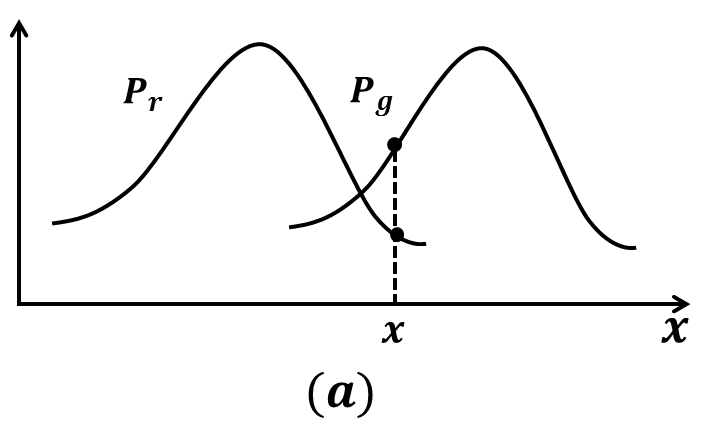
\includegraphics[width=4.5cm]{single_salmplein_2_equiv1}
            \qquad
            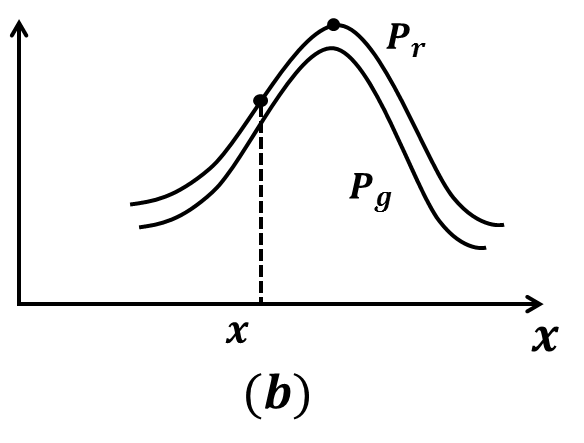
\includegraphics[width=4cm]{single_salmplein_2_equiv2}
            \caption{单一样本在2个分布中的概率值比较图}
            \label{fig:单一样本在2个分布中的概率值比较图}
            \end{figure}
            % \textcolor[rgb]{1 0 0}{todo:图片:单一样本在2个分布中的概率值比较图}\\
            当然,如果从单一样本的角度来看,从$P_g$中按概率抽取一个样本$x^*$,希望$x^*$和$\mathbb{E}_{x\sim P_r}(x)$接近,或者更近一步的说,我们希望两个总体$P_r,P_g$的均值相等。这变成了两总体均值相等检验问题,其示意图如图(\ref{fig:2总体均值是否相等示意图})所示
                \begin{figure}[H]
                \centering
                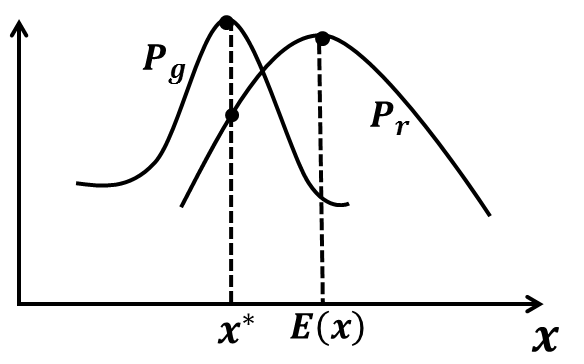
\includegraphics[width=4cm]{images/2_equiv.jpg}
                \caption{总体均值是否相等示意图}
                \label{fig:2总体均值是否相等示意图}
                \end{figure}
            % \textcolor[rgb]{1 0 0}{todo:图片:2总体均值是否相等示意图}\\
            \subsubsection{考虑固定的判别器D}
            \par
            现在,对于真假样本$x\sim P_r,x\sim P_g$,考虑一个判别器Ditector。并且,这里的判别器D是固定的,即D已经训练好了,在训练过程中D不再训练。而GAN中的D是需要训练的。我们从$P_g$中生成了$n$个样本$\{x_i\}_{i=1}^n$,从$P_r$中产生$n$个样本$\{x_i\}_{i=1}^n$,将二者混合在一起,输入到D中,对于每一个样本$x$,D都会给出$x$被判别为真的概率,记这个判别概率为$D(x)$($D(x)$是样本$x$被判为来自$P_r$的概率)。自然希望求G,使G带来的样本$x\sim P_g$被判为$P_r$的概率$D(x\sim P_g)$尽可能高(其实,没有必要将$x\sim P_r$输入到判别器D中),即
            \begin{align*}
            & \max _G\ \sum_{i=1}^n D(x_i)\\
            & s.t. \quad x_i\sim P_g,\quad i=1,2,\dots,n
            \end{align*}
            D中含有$P_r$的特征,当G能够欺骗D时,说明$P_g$也有了$P_r$的特征,进一步$x\sim P_g$可以充当$P_r$的样本。我们将上面的表达式写成平均值的形式,有
            \begin{align*}
            \max _G \ \frac{1}{n}\sum_{i=1}^n D(x_i) ,\quad x_i \sim P_g
            \end{align*}
            上式等价于
            \begin{align*}
            \max_G\ \mathbb{E}_{x\sim P_g} D(x)
            \end{align*}
            等价于
            \begin{align*}
            \min _G \ \mathbb{E}_{x\sim P_g}[1-D(x)]
            \end{align*}
            \par
            当然,我们可以将$D(x)$的形式进行变换,比如$\log D(x)$或者$\log (1-D(x))$。求解上面的优化问题,最终会得到一个G,我们称G是在D下的生成器,$P_g$是在D下的$P_r$的估计。
            \par
            在这一部分中,是在D的判别下让$x$使$P_r$的概率最大。回到前一部分,对于一个给定的$x\sim P_g$,我们也会有$x$在$P_r$中的概率,即假样本$x$在真分布$P_r$中的概率,如图(\ref{fig:假样本在真分布的概率示意图})所示
                \begin{figure}[H]
                \centering
                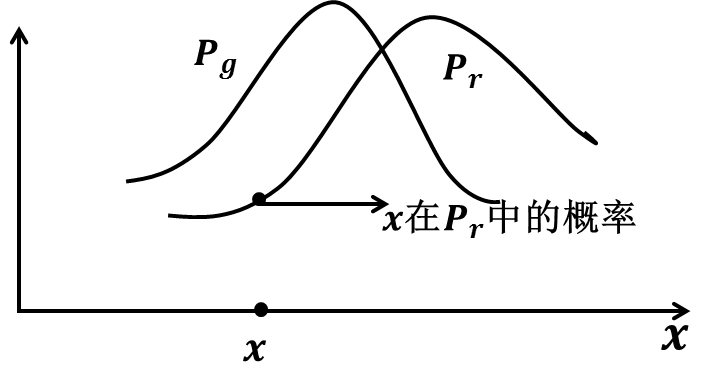
\includegraphics[width=5cm]{images/fault_sample_in_real_distribution.jpg}
                \caption{假样本在真分布的概率示意图}
                \label{fig:假样本在真分布的概率示意图}
                \end{figure}
            % \textcolor[rgb]{1 0 0 }{todo:图片:假样本在真分布的概率示意图}\\
            于是也可以设定目标
            \begin{align*}
            \max_G\ \mathbb{E}_{x\sim p_g}P_r(x)
            \end{align*}
            其中:$P_r(x)$表示样本$x\sim P_g$在$P_r$的概率。这里的$P_r$就充当了判别器D,而判别器D充当了极大似然估计中的似然函数(样本$x\sim P_g$在$P_r$或者D下出现的概率最大)。所以,在这一部分中,还可以对G设置联合概率最大的目标,如下
            \begin{align*}
            &\max_G\ D(x)_{x\sim P_g} = D(x_1)D(x_2)\cdots D(x_n)\\
            &\max_G\ P_r(x)_{x_1,\dots,x_n\overset{iid}{\sim }P_g} = P_r(x_1)P_r(x_2)\cdots P_r(x_n)
            \end{align*}
            注意到,生成器G的好坏与D的判别率有直接关系。
        \subsubsection{可变动的判别器D}
            \par
            在上一部分,我们设定判别器D是固定的,现在,假设在对真假样本$(x,x)$进行判别时,D也在不断的学习。
            \par
            在每次对G进行训练/迭代之前,我们都训练一下D。直观的说:第$t$次迭代时,从$P_g$中产生了$n$个样本,通过D判别后,找到了G的修正方案(梯度),然后G更新为G。在$t+1$次迭代时,从$P_g$中再次产生$n$个新样本,问题是:还用那个老旧的D来做判别吗?不!我们用一个新的D来做判别(可以再找其它的判别模型进行判别,还可以联合判别,这个之后再讨论),这里不打算换用其它类型的判别器,仍然在D上做,但要求$t+1$时刻的D更准确。我们需要训练D,要训练D则需要用于训练的样本数据,这里有两种方案:1种是样本不变,1种是将$x\sim P_g$加入到D的训练当中。采用第二种方案,将$x\sim P_g$的标签值设置为$-1$或$0$,表示“假”,然后训练D即可。
            \par
            当然,在GAN中,作者给D的训练设置了目标:要求D使$x\sim P_r$被判为真样本的概率$D(x\sim P_r)$尽可能大,$x\sim P_g$被判为真样本的概率$D(x\sim P_g)$尽可能小,即
            \begin{align*}
            \max \ \sum_{i=1}^n D(x_i)_{x_1,\dots,x_n\sim P_r}\\
            \min \ \sum_{i=1}^n D(x_i)_{x_1,\dots,x_n\sim P_g}
            \end{align*}
            将上式改为均值形式,有
            \begin{align*}
            \max_D\ \mathbb{E}_{x\sim P_r} D(x)\\
            \min_D\ \mathbb{E}_{x\sim P_g} D(x)
            \end{align*}
            其中,第二个目标等价于
            \begin{align*}
            \max_D\ \mathbb{E}_{x\sim P_g}[1-D(x)]
            \end{align*}
            将上述两个目标合并,有
            \begin{align*}
            \max _D\ \mathbb{E}_{x\sim P_r}[D(x)] + \mathbb{E}_{x\sim P_g}[1-D(x)]
            \end{align*}
            \par
            捋一下:当前时刻$t$更新完G之后$G_t$,在$t+1$时刻,要先训练一会儿D(得到$D_{t+1}$),然后再用新的$D_{t+1}$来进行判别,求G的更新方向$G_{t+1} = G_t+\Delta G_t$。对于G,我们的目标是
            \begin{align*}
            \min_G\ \mathbb{E}_{x\sim P_g}[1-D(x)]
            \end{align*}
            对于D,目标是
            \begin{align*}
            \max_D\ \mathbb{E}_{x\sim P_r}[D(x)]+\mathbb{E}_{x\sim P_g}[1-D(x)]
            \end{align*}
            \par
            将上述两个目标合并,形成二层规划或者最小最大规划,有
            \begin{align}
            \label{GAN模型1}
            \min_G\ \max_D\ \mathbb{E}_{x\sim P_r}[D(x)]+\mathbb{E}_{x\sim P_g}[1-D(x)]
            \end{align}

    \subsection{Vanilla GAN}
        \subsubsection{原始GAN模型}
            \par
            在GAN原文\cite{2014.Goodfellow}中,作者将上述目标(\ref{GAN模型1})的判别概率$D(x)$变为了$\log D(x)$,有
            \begin{align*}
            \min_G\ \max_D\ V(D,G) =  \mathbb{E}_{x\sim P_r}[\log D(x)]+\mathbb{E}_{x\sim P_g}[\log(1-D(x))]
            \end{align*}
            再将$x\sim P_g$改写为$x = G(z),z\sim U[0,1]$,将$U[0,1]$扩展为$P_z$,有
            \begin{align}
            \label{GAN原始目标}
            \min_G\ \max_D\ V(D,G) =  \mathbb{E}_{x\sim P_r}[\log D(x)]+\mathbb{E}_{z\sim P_z}[\log(1-D(G(z)))]
            \end{align}
            \par
            下面来分析一下GAN的优化模型(\ref{GAN原始目标})。对于$\min_G\max_D$,\ding{172}先固定G来看$\max_D$:
            \begin{theorem}[最优判别器D]
            在G固定的条件下,最优判别器D\footnote{注意,这里是密度函数$p_g,p_r$。}为
            \begin{align*}
            D_G^*(x) = \frac{p_r(x)}{p_r(x)+p_g(x)}
            \end{align*}
            \end{theorem}
            \begin{Proof}
            给定G,训练D就是求解
            \begin{align*}
            \max_D \ V(G,D) = \mathbb{E}_{x\sim P_r}[\log D(x)]+\mathbb{E}_{z\sim P_z}[\log(1-D(G(z)))]
            \end{align*}
            而
            \begin{align*}
            V(G,D) &= \int_x p_r(x) \log D(x)\mathrm{d}x + \int_z p_z(z)\log(1-D(G(z)))\mathrm{d}z\\
            &=\int_x p_r(x)\log D(x)+ p_g(x)\log(1-D(x))\mathrm{d}x
            \end{align*}
            对于函数$a\log(y)+b\log(1-y)$,$\forall (a,b)\in R^2/\{0,0\}$在$[0,1]$处取得最大值$\frac{a}{a+b}$。
            \end{Proof}
            \par
            \ding{173}在得到最优判别器$D^*$的情况下,来求$\min_G\ V(G,D^*)$。我们先将$D^*$带入到$V(G,D)$,有
            \begin{align*}
            V(G,D^*) &= \mathbb{E}_{x\sim P_r}[\log D^*(x)] + \mathbb{E}_{z\sim P_z}[\log (1-D^*(G(z)))]\\
            &=\mathbb{E}_{x\sim P_r}[\log D^*(x)]+\mathbb{E}_{x\sim P_g}[\log (1-D^*(x))]\\
            &=\mathbb{E}_{x\sim P_r} \left[ \log \frac{p_r(x)}{p_r(x)+p_g(x)} \right] + \mathbb{E}_{x\sim P_g} \left[\log \frac{p_g(x)}{p_r(x)+p_g(x)}   \right]
            \end{align*}
            令$C(G) = V(G,D^*)$,则要求$\min_G\ C(G)$。
            \begin{theorem}
            当且仅当$p_r = p_g$时,$C(G)$有全局极小点,且$C(G)$在此点处的值为$-\log 4$。
            \end{theorem}
            \begin{Proof}
            考虑$p_g = p_r$,则$D^*(x) = \frac{1}{2}$,于是
            \begin{align*}
            C(G) & = \log \frac{1}{2}+\log \frac{1}{2} = -\log 4\\
            & = \mathbb{E}_{x\sim P_r}(-\log 2)+\mathbb{E}_{x\sim P_g}(-\log 2)
            \end{align*}
            为了表明$p_g = p_r$是最小点,$-\log 4$是最小值,我们将$C(G)$减去$-\log 4$。如果$C(G)+\log 4 \geqslant 0$,则表明$C(G)$的最小值为$-\log 4$。
            \begin{align*}
            C(G) & = -\log 4 + KL \left( P_r\Big|\Big| \frac{P_r+P_g}{2} \right) + KL \left( P_g\Big|\Big| \frac{P_r+P_g}{2} \right) \\
            & = -\log 4+ 2JSD(P_r||P_g)
            \end{align*}
            由JSD散度(Jensen Shannon Dirergence)\footnote{For distributions $P$ and $Q$ of a continuous random variable, the Kullback–Leibler divergence is defined to be the integral
            \begin{align*}
            KL(P||Q) = \int_{-\infty}^\infty p(x) \log \frac{p(x)}{q(x)}\mathrm{d}x
            \end{align*}
            where$ p $and$ q $denote the densities of$ P $and$ Q$.
             }
            可知,当且仅当$p_r = p_g$时JSD = 0,否则JSD$>0$。于是$C(G) \geqslant 0$,当且仅当$p_r = p_g$时,等号成立。
            \end{Proof}
            \par
            回看上面的证明,我们会发现,在D给定后,求G就是求$\min _G C(G)$。而$C(G)$去掉他的极小值后,就是一个$P_r,P_g$的JSD散度,所以,我们求G的本质是求
            \begin{align*}
            \min _G\ JSD(P_r||P_g) = KL \left( P_r\Big|\Big| \frac{P_r+P_g}{2} \right) + KL \left( P_G\Big|\Big| \frac{P_r+P_g}{2} \right)
            \end{align*}
            自然会考虑能否为G设置其他的散度或距离(D的目标基本不变)\footnote{https://en.wikipedia.org/wiki/Kullback\%E2\%80\%93Leibler\_divergence},这将在后面的$f$-GAN中进行详细说明。下面,给出GAN的程序。
        \subsubsection{GAN算法与程序}
            \par
            GAN的伪代码如(\ref{code:Vanilla GAN})所示
            \begin{algorithm}[htbp]
                \caption{Minibatch stochastic gradient descent training of GAN}\label{code:Vanilla GAN}
                \begin{algorithmic}[1]
                    \State 初始化:$P_r$的真实样本$\{x_i\}_{i=1}^n$(即原有的样本数据),迭代步$t$,$t_max$,生成器G判别器D,设G和D的参数为$\theta_g,\theta_d$,每迭代步$t$下,判别器训练次数$k$(即在一次更新G下,要更新$k$次D),批量大小$m$。
                    \For {$t=1,2,\dots,t_{max}$}
                        \State $//$更新D
                        \For {$k$ steps}
                            \State sample minibatch of m noise sample $\{z^{(1)},z^{(2)},\dots,z^{(m)}\}$ from $P_z$;生成$m$个假样本$x^{(1)} = G(z^{(1)}),x^{(2)} = G(z^{(2)}),\dots,x^{(m)} = G(z^{(m)})$。
                            \State sample minibatch of m example $\{x^{(1)},x^{(2)},\dots,x^{(m)}\}$ from $P_r$。即从原始数据$\{x_i\}_{i=1}^n$中挑出$m$个。
                            \State 将$2m$个真假样本$x^{(i)}$输入到判别器D,得到各样本属于真实分布的概率$D(x^{(i)})$
                            \begin{align*}
                            \max_D\ V(D,G) = \mathbb{E}_{x\sim P_r}[\log D(x)]+\mathbb{E}_{z\sim P_z}[\log (1-D(G(z)))]
                            \end{align*}
                            \State 求D的梯度
                            \begin{align*}
                            &\nabla _{\theta_d} \frac{1}{m} \sum_{i=1}^m [\log D_t(x^{(i)})]+\nabla_{\theta_d} \frac{1}{m} \sum_{i=1}^m [\log (1-D_t(G_t(z^{(i)})))]\\
                            ={}&\nabla_{\theta_d} \frac{1}{m} \sum_{i=1}^m [\log D_t(x^{(i)})+\log (1-D_t(G_t(z^{(i)})))]
                            \end{align*}
                            \State 求$D_{t+1} = D_t+\nabla_{\theta_d}$;
                        \EndFor
                        \State $//$ 更新G
                        \State sample minibatch of m noise sample $\{z^{(1)},z^{(2)},\dots,z^{(m)}\}$ from $P_z$;
                        \State 计算梯度
                        \begin{align*}
                        \nabla _{\theta_g}\frac{1}{m}\sum_{i=1}^m \log (1-D_{t+1}(G(z^{(i)})))
                        \end{align*}
                        \State 更新$G$
                        \begin{align*}
                        G_{t+1} = G_t + \nabla_{\theta_g}
                        \end{align*}
                    \EndFor
                \end{algorithmic}
            \end{algorithm}
            \par
            GAN模型的TensorFlow\footnote{http://www.tensorfly.cn/}\footnote{https://www.tensorflow.org/}程序如下,更详细的可以参考\footnote{https://github.com/wiseodd/generative-models/tree/master/GAN}
            \begin{lstlisting}[language = Python]
            import tensorflow as tf
            from tensorflow.examples.tutorials.mnist import input_data
            import numpy as np
            import matplotlib.pyplot as plt
            import matplotlib.gridspec as gridspec
            import os
            def xavier_init(size):
                in_dim = size[0]
                xavier_stddev = 1. / tf.sqrt(in_dim / 2.)
                return tf.random_normal(shape=size, stddev=xavier_stddev)
            X = tf.placeholder(tf.float32, shape=[None, 784])
            D_W1 = tf.Variable(xavier_init([784, 128]))
            D_b1 = tf.Variable(tf.zeros(shape=[128]))
            D_W2 = tf.Variable(xavier_init([128, 1]))
            D_b2 = tf.Variable(tf.zeros(shape=[1]))
            theta_D = [D_W1, D_W2, D_b1, D_b2]
            Z = tf.placeholder(tf.float32, shape=[None, 100])
            G_W1 = tf.Variable(xavier_init([100, 128]))
            G_b1 = tf.Variable(tf.zeros(shape=[128]))
            G_W2 = tf.Variable(xavier_init([128, 784]))
            G_b2 = tf.Variable(tf.zeros(shape=[784]))
            theta_G = [G_W1, G_W2, G_b1, G_b2]
            def sample_Z(m, n):
                return np.random.uniform(-1., 1., size=[m, n])
            def generator(z):
                G_h1 = tf.nn.relu(tf.matmul(z, G_W1) + G_b1)
                G_log_prob = tf.matmul(G_h1, G_W2) + G_b2
                G_prob = tf.nn.sigmoid(G_log_prob)
                return G_prob
            def discriminator(x):
                D_h1 = tf.nn.relu(tf.matmul(x, D_W1) + D_b1)
                D_logit = tf.matmul(D_h1, D_W2) + D_b2
                D_prob = tf.nn.sigmoid(D_logit)
                return D_prob, D_logit
            def plot(samples):
                fig = plt.figure(figsize=(4, 4))
                gs = gridspec.GridSpec(4, 4)
                gs.update(wspace=0.05, hspace=0.05)
                for i, sample in enumerate(samples):
                    ax = plt.subplot(gs[i])
                    plt.axis('off')
                    ax.set_xticklabels([])
                    ax.set_yticklabels([])
                    ax.set_aspect('equal')
                    plt.imshow(sample.reshape(28, 28), cmap='Greys_r')
                return fig
            G_sample = generator(Z)
            D_real, D_logit_real = discriminator(X)
            D_fake, D_logit_fake = discriminator(G_sample)
            # D_loss = -tf.reduce_mean(tf.log(D_real) + tf.log(1. - D_fake))
            # G_loss = -tf.reduce_mean(tf.log(D_fake))
            # Alternative losses:
            # -------------------
            D_loss_real = tf.reduce_mean(tf.nn.sigmoid_cross_entropy_with_logits(logits=D_logit_real, labels=tf.ones_like(D_logit_real)))
            D_loss_fake = tf.reduce_mean(tf.nn.sigmoid_cross_entropy_with_logits(logits=D_logit_fake, labels=tf.zeros_like(D_logit_fake)))
            D_loss = D_loss_real + D_loss_fake
            G_loss = tf.reduce_mean(tf.nn.sigmoid_cross_entropy_with_logits(logits=D_logit_fake, labels=tf.ones_like(D_logit_fake)))
            D_solver = tf.train.AdamOptimizer().minimize(D_loss, var_list=theta_D)
            G_solver = tf.train.AdamOptimizer().minimize(G_loss, var_list=theta_G)
            mb_size = 128
            Z_dim = 100
            mnist = input_data.read_data_sets('../../MNIST_data', one_hot=True)
            sess = tf.Session()
            sess.run(tf.global_variables_initializer())
            if not os.path.exists('out/'):
                os.makedirs('out/')
            i = 0
            for it in range(1000000):
                if it % 1000 == 0:
                    samples = sess.run(G_sample, feed_dict={Z: sample_Z(16, Z_dim)})

                    fig = plot(samples)
                    plt.savefig('out/{}.png'.format(str(i).zfill(3)), bbox_inches='tight')
                    i += 1
                    plt.close(fig)
                X_mb, _ = mnist.train.next_batch(mb_size)
                _, D_loss_curr = sess.run([D_solver, D_loss], feed_dict={X: X_mb, Z: sample_Z(mb_size, Z_dim)})
                _, G_loss_curr = sess.run([G_solver, G_loss], feed_dict={Z: sample_Z(mb_size, Z_dim)})
                if it % 1000 == 0:
                    print('Iter: {}'.format(it))
                    print('D loss: {:.4}'. format(D_loss_curr))
                    print('G_loss: {:.4}'.format(G_loss_curr))
            print()
            \end{lstlisting}

    \subsection{f-GAN}
        \par
        文献\cite{2016.Sebastian}中介绍了一些“可行”的divergence和distance(注意:距离和散度不是同一概念,距离是对称的而散度不是),并且Sebastian等也从变分角度给出了设置判别器D的原因。
        \subsubsection{f-散度族}
            \par
            KL距离可能是最为常用的散度了,它用于衡量2个概率分布$P_r,P_g$的不同程度。现在,我们来介绍一大类散度:$f$-散度族。令$x$为随机变量,$\mathcal{X}$是其取值域(domain),$f$-散度定义为
            \begin{align*}
            D_f(P_r||P_g) = \int_\mathcal{X}p_g(x)f \left( \frac{p_r(x)}{p_g(x)} \right) \mathrm{d}x
            \end{align*}
            其中:$f:R^+\to R$是一个凸的单调函数,满足$f(1) = 0$。$f$不同,最终的距离/散度$D_f(P_r||P_g)$就不同。常见的$f$以及由其形成的$D_f(P_r||P_g)$如图(\ref{fig:f散度族})所示
                \begin{figure}[H]
                \centering
                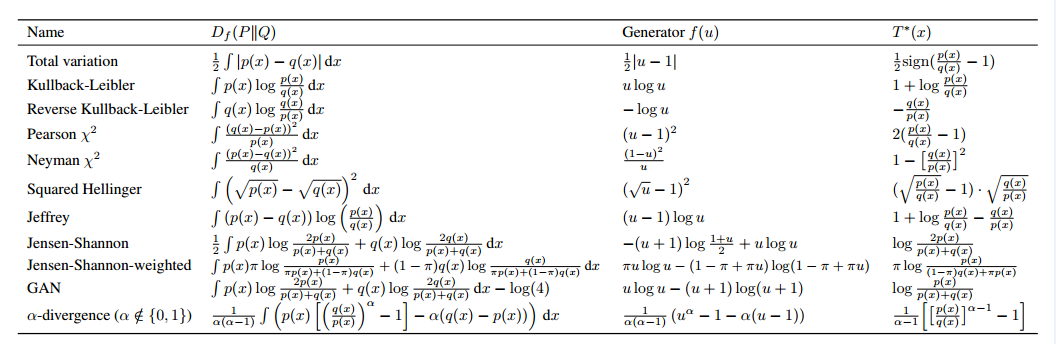
\includegraphics[width=15cm]{images/fsandu1.jpg}
                \caption{f散度族}
                \label{fig:f散度族}
                \end{figure}
            % \textcolor[rgb]{1 0 0}{todo:表格:f散度族}\\
            其中:$u$是$f$的自变量,$dom_f$表示$f$的自变量域,即$u$的域。下面,我们来看$f$散度的变分估计。
        \subsubsection{Veriational Estimation of f-divergence}
            \par
            在GAN中求解G时,使用上面介绍的$f$散度,目标变为求G使$D_f(P_r||P_g)$最小,有
            \begin{align*}
            \min_G\ D_f(P_r||P_g) = \int_\mathcal{X}p_g(x)f \left( \frac{p_r(x)}{p_g(x)} \right) \mathrm{d}x
            \end{align*}
            此时的G中还不具有参数,因此上述问题是一个关于$P_g$的变分问题。Nguyen讨论了在只有$P_g,P_r$(无$f$)时,$f$-divergence的一个一般化的变分估计方法。下面,我们将会用变分估计方法来求解G (将$P_g$参数化后求参数$\theta_g$)。为了完整,我们给出Nguyan散度估计的一个self-containde:
            \par
            对于任意一个凸的单调函数$f$,有一个凸共轭(conjugate)函数$f^*$,也被称为fenchel共轭。定义为
            \begin{align*}
            f^*(t) = \sup_{u\in dom_f}\{ut - f(u)\}
            \end{align*}
            并且,$f^*$也是凸的单调的。对于这对函数$(f,f^*)$,有$f^{**} = f$。因此,可以将$f$表示为
            \begin{align*}
            f(u) = \sup_{t\in dom_{f^*}} \{tu - f^*(t)\}
            \end{align*}
            将$f(u)$带入到$D_f(P_r||P_g)$中,有(这里的$u$是$\frac{p_r(x)}{p_g(x)}$)
            \begin{align*}
            D_f(P_r||P_g) & = \int_\mathcal{X} p_g(x )f \left( \frac{p_r(x)}{p_g(x)} \right)\mathrm{d}x\\
            & =\int _\mathcal{X} p_g(x) \sup_{t\in dom_{f^*}} \left\{t\frac{p_r(x)}{p_g(x)} - f^*(t)\right\} \mathrm{d}x \\
            &\geqslant \sup_{t\in dom_{f^*}}\int_\mathcal{X} p_g(x) t\frac{p_r(x)}{p_g(x)} - p_g(x)f^*(t)\mathrm{d}x \quad \text{Jensen不等式}\\
            &\geqslant \sup _{T\in \Gamma} \left( \int_\mathcal{X}p_r(x)T(x)\mathrm{d}x - \int_\mathcal{X} p_g(x)f^*(T(x))\mathrm{d}x \right)\\
            & = \sup _{T\in \Gamma} \left( \mathbb{E}_{x\sim  P_r}[T(x)] - \mathbb{E}_{x\sim  P_g}[f^*(T(x))] \right)
            \end{align*}
            其中:$T(x):\mathcal{X}\to R$是$\mathcal{X}$上的函数,$\Gamma$是$T$的任意一个函数集,且是无穷维函数空间(T的所有可能)的一个小部分(subset),因此有第二个不等号。
            \par
            可以发现,这里的$T$就相当于GAN中的分类器D。计算上式得变分下界,我们发现,在可能的函数集$\Gamma$中,the bound is tight for
            \begin{align*}
            T^*(x) = f' \left( \frac{p_r(x)}{p_g(x)} \right)
            \end{align*}
            其中:$f'$是$f$的一阶导。这个情况可以用于指导我们如何选择$f$以及设计函数集$\Gamma$。例如:KL散度相当于$f(u) = -\log (u)$,其下界为$T^*(x) = -\frac{p_g(x)}{p_r(x)}$,图(\ref{fig:f散度族})中给出了一些$f$散度,图(\ref{fig:f散度的共轭})给出了共轭$f^*$以及$f^*$的域$dom_{f^*}$。
                \begin{figure}[H]
                \centering
                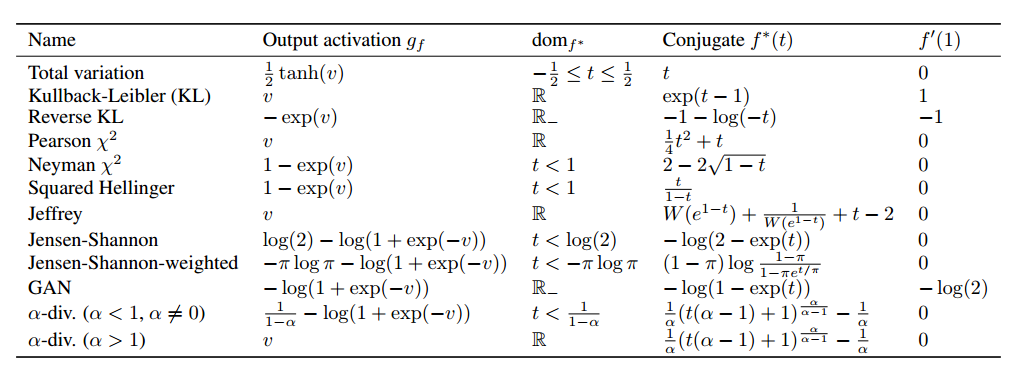
\includegraphics[width=12cm]{images/fsandu.jpg}
                \caption{f散度的共轭}
                \label{fig:f散度的共轭}
                \end{figure}
            % \textcolor[rgb]{1 0 0}{todo:图片:f散度的共轭}
            \par
            上述问题仍然是一个泛函(变分)问题
            \begin{align*}
            \min_{P_g} \ \sup_{T}\ V(P_r,T) = \mathbb{E}_{x\sim P_r}[T(x)] - \mathbb{E}_{x\sim P_g}[f^*(T(x))]
            \end{align*}
            下面来处理这个泛函问题。像一般的泛函问题那样,将函数问题参数化,将求函数问题变为求参数问题。将两个函数$P_g \triangleq G $和$T\triangleq D$参数化,设其参数为$\theta_g,\theta_d$,于是有
            \begin{align*}
            \min_{\theta_g} \ \max_{\theta_d}\ F(\theta_g,\theta_d) = \mathbb{E}_{x\sim P_r}[T_{\theta_d}(x)] - \mathbb{E}_{x\sim P_{\theta_g}}[f^*(T_{\theta_d}(x))]
            \end{align*}
            \par
            为了书写方便,令$(\theta_g,\theta_d) \triangleq (\theta,w)$,$T_w(x)  = g_f(V_w(x))$,于是上述目标变为
            \begin{align*}
            \min_\theta \ \max_w \ F(\theta,w) = \mathbb{E}_{x\sim P_r}[g_f(V_w(x))] + \mathbb{E}_{x\sim P_g}[-f^*(g_fV_w(x))]
            \end{align*}
            其中:$V_w:\mathcal{X}\to R$的输出$R$不存在任何限制,$g_f:R\to dom_{f^*}$是一个输出激活函数。
        \subsubsection{f-GAN的程序}
            \par
            f-GAN的TensorFlow程序如下
            \begin{lstlisting}[language = Python]
            import tensorflow as tf
            from tensorflow.examples.tutorials.mnist import input_data
            import numpy as np
            import matplotlib.pyplot as plt
            import matplotlib.gridspec as gridspec
            import os
            mb_size = 32
            X_dim = 784
            z_dim = 64
            h_dim = 128
            lr = 1e-3
            d_steps = 3
            mnist = input_data.read_data_sets('../../MNIST_data', one_hot=True)
            def plot(samples):
                fig = plt.figure(figsize=(4, 4))
                gs = gridspec.GridSpec(4, 4)
                gs.update(wspace=0.05, hspace=0.05)
                for i, sample in enumerate(samples):
                    ax = plt.subplot(gs[i])
                    plt.axis('off')
                    ax.set_xticklabels([])
                    ax.set_yticklabels([])
                    ax.set_aspect('equal')
                    plt.imshow(sample.reshape(28, 28), cmap='Greys_r')
                return fig
            def xavier_init(size):
                in_dim = size[0]
                xavier_stddev = 1. / tf.sqrt(in_dim / 2.)
                return tf.random_normal(shape=size, stddev=xavier_stddev)
            X = tf.placeholder(tf.float32, shape=[None, X_dim])
            z = tf.placeholder(tf.float32, shape=[None, z_dim])
            D_W1 = tf.Variable(xavier_init([X_dim, h_dim]))
            D_b1 = tf.Variable(tf.zeros(shape=[h_dim]))
            D_W2 = tf.Variable(xavier_init([h_dim, 1]))
            D_b2 = tf.Variable(tf.zeros(shape=[1]))
            G_W1 = tf.Variable(xavier_init([z_dim, h_dim]))
            G_b1 = tf.Variable(tf.zeros(shape=[h_dim]))
            G_W2 = tf.Variable(xavier_init([h_dim, X_dim]))
            G_b2 = tf.Variable(tf.zeros(shape=[X_dim]))
            theta_G = [G_W1, G_W2, G_b1, G_b2]
            theta_D = [D_W1, D_W2, D_b1, D_b2]
            def sample_z(m, n):
                return np.random.uniform(-1., 1., size=[m, n])
            def generator(z):
                G_h1 = tf.nn.relu(tf.matmul(z, G_W1) + G_b1)
                G_log_prob = tf.matmul(G_h1, G_W2) + G_b2
                G_prob = tf.nn.sigmoid(G_log_prob)
                return G_prob
            def discriminator(x):
                D_h1 = tf.nn.relu(tf.matmul(x, D_W1) + D_b1)
                out = tf.matmul(D_h1, D_W2) + D_b2
                return out
            G_sample = generator(z)
            D_real = discriminator(X)
            D_fake = discriminator(G_sample)
            # Uncomment D_loss and its respective G_loss of your choice
            # ---------------------------------------------------------
            """ Total Variation """
            # D_loss = -(tf.reduce_mean(0.5 * tf.nn.tanh(D_real)) -
            #            tf.reduce_mean(0.5 * tf.nn.tanh(D_fake)))
            # G_loss = -tf.reduce_mean(0.5 * tf.nn.tanh(D_fake))
            """ Forward KL """
            # D_loss = -(tf.reduce_mean(D_real) - tf.reduce_mean(tf.exp(D_fake - 1)))
            # G_loss = -tf.reduce_mean(tf.exp(D_fake - 1))
            """ Reverse KL """
            # D_loss = -(tf.reduce_mean(-tf.exp(D_real)) - tf.reduce_mean(-1 - D_fake))
            # G_loss = -tf.reduce_mean(-1 - D_fake)
            """ Pearson Chi-squared """
            D_loss = -(tf.reduce_mean(D_real) - tf.reduce_mean(0.25*D_fake**2 + D_fake))
            G_loss = -tf.reduce_mean(0.25*D_fake**2 + D_fake)
            """ Squared Hellinger """
            # D_loss = -(tf.reduce_mean(1 - tf.exp(D_real)) -
            #            tf.reduce_mean((1 - tf.exp(D_fake)) / (tf.exp(D_fake))))
            # G_loss = -tf.reduce_mean((1 - tf.exp(D_fake)) / (tf.exp(D_fake)))

            D_solver = (tf.train.AdamOptimizer(learning_rate=lr)
                        .minimize(D_loss, var_list=theta_D))
            G_solver = (tf.train.AdamOptimizer(learning_rate=lr)
                        .minimize(G_loss, var_list=theta_G))
            sess = tf.Session()
            sess.run(tf.global_variables_initializer())
            if not os.path.exists('out/'):
                os.makedirs('out/')
            i = 0
            for it in range(1000000):
                X_mb, _ = mnist.train.next_batch(mb_size)
                z_mb = sample_z(mb_size, z_dim)
                _, D_loss_curr = sess.run([D_solver, D_loss], feed_dict={X: X_mb, z: z_mb})
                _, G_loss_curr = sess.run([G_solver, G_loss], feed_dict={z: z_mb})
                if it % 1000 == 0:
                    print('Iter: {}; D_loss: {:.4}; G_loss: {:.4}'
                          .format(it, D_loss_curr, G_loss_curr))
                    samples = sess.run(G_sample, feed_dict={z: sample_z(16, z_dim)})
                    fig = plot(samples)
                    plt.savefig('out/{}.png'
                                .format(str(i).zfill(3)), bbox_inches='tight')
                    i += 1
            plt.close(fig)
            \end{lstlisting}

    \subsection{Conditional GAN}
        \par
        回顾前面的GAN,在生成假样本$x\sim P_g$时,用$x = G(z),z\sim U[0,1]$,即生成器G的网络输入仅是随机值$z$。现在,考虑能否将其它信息作为G的输入来生成假样本$x$,即生成网络的输入$z$变为其它形式(还可以考虑G在生成$x$的同时还生成其它信息,这个后面讨论)。可以尝试用$z\sim N$来替代原本的$z\sim U$,这是行的通的,并且也可以解释的通(下面解释)。但是,即便是$z\sim f$,GAN仍然是一个无指导性的生成:训练后的GAN只能生成room图片,而不能根据要求生成相应的图片(比如要求GAN生成狗的图片,再生成猫的图片)。
        \par
        现在,考虑这样一种生成问题:用同一个GAN,生成数字1、数字2$\cdots$,即我们来指导GAN生成哪些事物,称这些指导为指导信息。我们将指导信息作为输入来生成假样本$x$。
        \par
        在介绍CGAN之前,先来考虑一般的图像回归/分类问题$X\to Y$,构建回归器
        \begin{align*}
        & y = w \phi(x)+z\\
        & z\sim N(0,\sigma^2)
        \end{align*}
        更一般的,记为$y = \varphi(x)+z$。既然可以从$X\to Y$,我们同样可以用神经网络来构建$Y\to X$的映射,有
        \begin{align*}
        x = G(y)+z
        \end{align*}
        这里的$y$即为图像的标签信息。在图像分类任务中,我们将图片$x$作为输入,标签值$y$作为输出,构建$X\to Y$的映射,现在反过来,以$y$为输入,$x$为输出,构建$Y\to X$的映射以生成图像(一个很普通的问题是:当$y$和$z$的维度很低时,要生成高维$x$是不易的)。
        \par
        要从$x = G(y)+z$中采样($y = \varphi(x)+z$中采样是一样的),我们都只需要取一个$y$形成$G(y)$,再生成多个随机值$z$,将$G(y)$和多个随机值$z$相加,求平均即可,即$x_i = \sum_{j}G(y_i)+z_{ij} $。
        \begin{align*}
        p_g(x) & = \int _z p(x,z)\mathrm{d}z\\
        & =\int_z p(x|z)p(z)\mathrm{d}z\\
        & =\sum_zp(x|z)p(z)
        \end{align*}
        更一般的\cite{2014.Mirza},在输入层中加入噪声$z$,如图(\ref{fig:CGAN生成网络示意图})所示
                \begin{figure}[H]
                \centering
                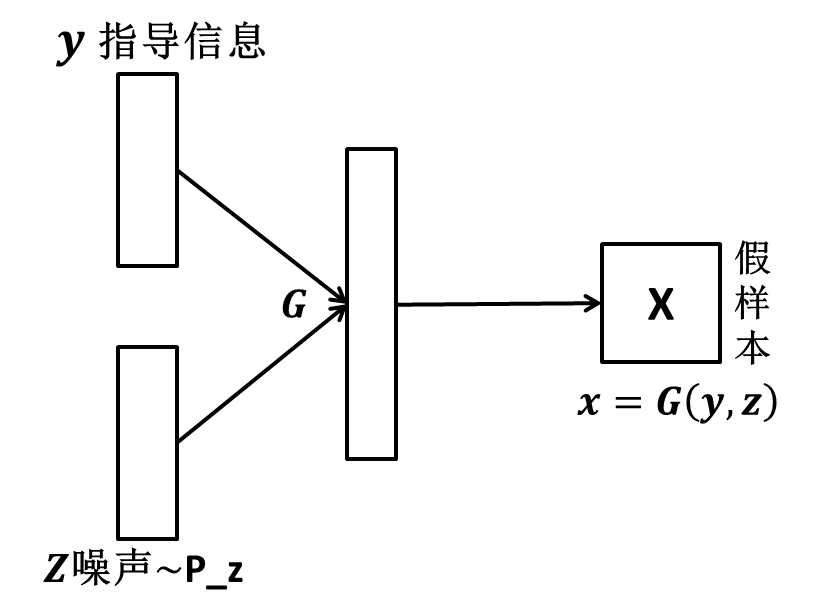
\includegraphics[width=5cm]{images/CGAN_product_network.jpg}
                \caption{CGAN生成网络示意图}
                \label{fig:CGAN生成网络示意图}
                \end{figure}
        % \textcolor[rgb]{1 0 0}{todo:图片:CGAN生成网络示意图}\\
        $x = G(z,y)$。注意,这里和前面DAE中添加噪声的方法有所不同,DAE是在$x$中添加噪声,形成$\tilde{x} = x+z$,而这里是将$z$作为输入的一部分。
        \par
        在判别器D中,将$y$作为输入,$x$作为输入来进行判别,$D(x|y)$表示$y$给定后,输入样本$x$为真的概率。这里有一个问题:判别器D的输入和输出是什么?\ding{172}输入为标签值$y$,输出为$p(x|y)$,表示输入$y$输出为$x$的条件概率。\ding{173}输入是$(y,x)$,输出是$D(x|y)$,表示输入$y,x$为真的概率。如果是第一种方法,则G和D作的任务是一样的。采用第二种方法,CGAN的网络结构图如图(\ref{fig:CGAN网络结构图})所示
                \begin{figure}[H]
                \centering
                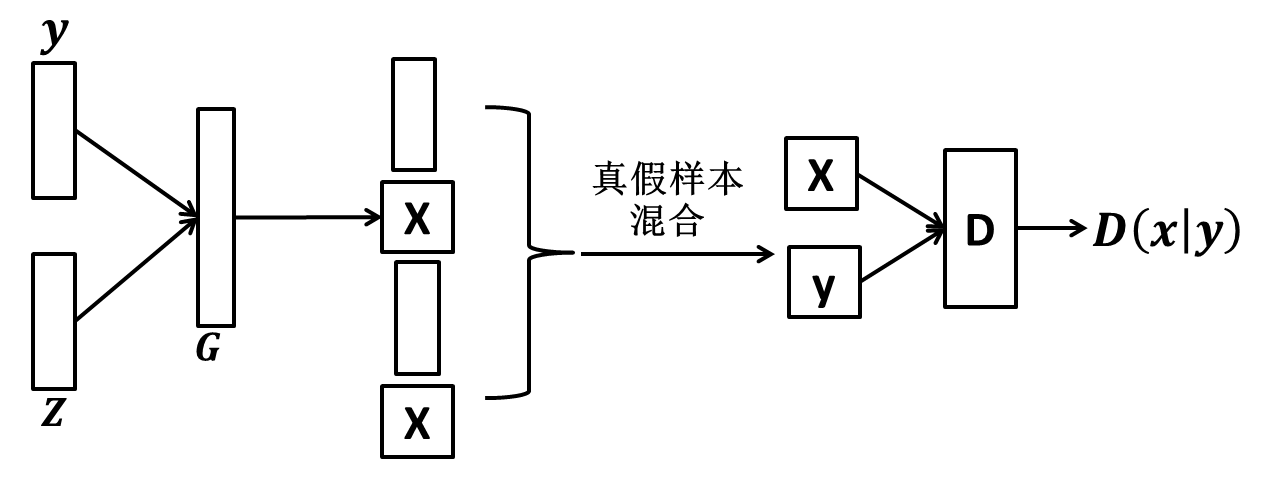
\includegraphics[width=8cm]{images/CGAN_network.jpg}
                \caption{CGAN网络结构图}
                \label{fig:CGAN网络结构图}
                \end{figure}
        % \textcolor[rgb]{1 0 0}{todo:图片:CGAN网络结构图}\\
        可以构建如下条件GAN(CGAN)的目标
        \begin{align*}
        \min_G\ \max_D\ V(D,G) & = \mathbb{E}_{x\sim P_r}[\log D(x|y)] + \mathbb{E}_{z\sim P_z}[\log (1-D(x|y))]\\
        & = \mathbb{E}_{x\sim P_r}[\log D(x|y)] + \mathbb{E}_{z\sim P_z}[\log (1-D(G(z,y)|y))]
        \end{align*}
        值得一提的是,CGAN中的$z$可以是任意的噪声,不局限于均匀噪声$z\sim U[0,1]$。CGAN的TensorFolw程序如下
        \begin{lstlisting}[language = Python]
        import tensorflow as tf
        from tensorflow.examples.tutorials.mnist import input_data
        import numpy as np
        import matplotlib.pyplot as plt
        import matplotlib.gridspec as gridspec
        import os
        mnist = input_data.read_data_sets('../../MNIST_data', one_hot=True)
        mb_size = 64
        Z_dim = 100
        X_dim = mnist.train.images.shape[1]
        y_dim = mnist.train.labels.shape[1]
        h_dim = 128
        def xavier_init(size):
            in_dim = size[0]
            xavier_stddev = 1. / tf.sqrt(in_dim / 2.)
            return tf.random_normal(shape=size, stddev=xavier_stddev)
        """ Discriminator Net model """
        X = tf.placeholder(tf.float32, shape=[None, 784])
        y = tf.placeholder(tf.float32, shape=[None, y_dim])
        D_W1 = tf.Variable(xavier_init([X_dim + y_dim, h_dim]))
        D_b1 = tf.Variable(tf.zeros(shape=[h_dim]))
        D_W2 = tf.Variable(xavier_init([h_dim, 1]))
        D_b2 = tf.Variable(tf.zeros(shape=[1]))
        theta_D = [D_W1, D_W2, D_b1, D_b2]
        def discriminator(x, y):
            inputs = tf.concat(axis=1, values=[x, y])
            D_h1 = tf.nn.relu(tf.matmul(inputs, D_W1) + D_b1)
            D_logit = tf.matmul(D_h1, D_W2) + D_b2
            D_prob = tf.nn.sigmoid(D_logit)
            return D_prob, D_logit
        """ Generator Net model """
        Z = tf.placeholder(tf.float32, shape=[None, Z_dim])
        G_W1 = tf.Variable(xavier_init([Z_dim + y_dim, h_dim]))
        G_b1 = tf.Variable(tf.zeros(shape=[h_dim]))
        G_W2 = tf.Variable(xavier_init([h_dim, X_dim]))
        G_b2 = tf.Variable(tf.zeros(shape=[X_dim]))
        theta_G = [G_W1, G_W2, G_b1, G_b2]
        def generator(z, y):
            inputs = tf.concat(axis=1, values=[z, y])
            G_h1 = tf.nn.relu(tf.matmul(inputs, G_W1) + G_b1)
            G_log_prob = tf.matmul(G_h1, G_W2) + G_b2
            G_prob = tf.nn.sigmoid(G_log_prob)
            return G_prob
        def sample_Z(m, n):
            return np.random.uniform(-1., 1., size=[m, n])
        def plot(samples):
            fig = plt.figure(figsize=(4, 4))
            gs = gridspec.GridSpec(4, 4)
            gs.update(wspace=0.05, hspace=0.05)
            for i, sample in enumerate(samples):
                ax = plt.subplot(gs[i])
                plt.axis('off')
                ax.set_xticklabels([])
                ax.set_yticklabels([])
                ax.set_aspect('equal')
                plt.imshow(sample.reshape(28, 28), cmap='Greys_r')
            return fig
        G_sample = generator(Z, y)
        D_real, D_logit_real = discriminator(X, y)
        D_fake, D_logit_fake = discriminator(G_sample, y)
        D_loss_real = tf.reduce_mean(tf.nn.sigmoid_cross_entropy_with_logits(logits=D_logit_real, labels=tf.ones_like(D_logit_real)))
        D_loss_fake = tf.reduce_mean(tf.nn.sigmoid_cross_entropy_with_logits(logits=D_logit_fake, labels=tf.zeros_like(D_logit_fake)))
        D_loss = D_loss_real + D_loss_fake
        G_loss = tf.reduce_mean(tf.nn.sigmoid_cross_entropy_with_logits(logits=D_logit_fake, labels=tf.ones_like(D_logit_fake)))
        D_solver = tf.train.AdamOptimizer().minimize(D_loss, var_list=theta_D)
        G_solver = tf.train.AdamOptimizer().minimize(G_loss, var_list=theta_G)
        sess = tf.Session()
        sess.run(tf.global_variables_initializer())
        if not os.path.exists('out/'):
            os.makedirs('out/')
        i = 0
        for it in range(1000000):
            if it % 1000 == 0:
                n_sample = 16
                Z_sample = sample_Z(n_sample, Z_dim)
                y_sample = np.zeros(shape=[n_sample, y_dim])
                y_sample[:, 7] = 1
                samples = sess.run(G_sample, feed_dict={Z: Z_sample, y:y_sample})
                fig = plot(samples)
                plt.savefig('out/{}.png'.format(str(i).zfill(3)), bbox_inches='tight')
                i += 1
                plt.close(fig)
            X_mb, y_mb = mnist.train.next_batch(mb_size)
            Z_sample = sample_Z(mb_size, Z_dim)
            _, D_loss_curr = sess.run([D_solver, D_loss], feed_dict={X: X_mb, Z: Z_sample, y:y_mb})
            _, G_loss_curr = sess.run([G_solver, G_loss], feed_dict={Z: Z_sample, y:y_mb})
            if it % 1000 == 0:
                print('Iter: {}'.format(it))
                print('D loss: {:.4}'. format(D_loss_curr))
                print('G_loss: {:.4}'.format(G_loss_curr))
        print()
        \end{lstlisting}
        \par
        实验:在MINIST数据集上,以类别标签为条件$y$(one - hot编码),给定$z$后,生成0-9数字图像,然后将$(y,x|y)\sim P_g$,$(y,x|y)\sim P_r$作为训练集输入到D中进行判断。最终生成的0-9数字图像如图(\ref{fig:CGAN数字生成图})所示
                \begin{figure}[H]
                \centering
                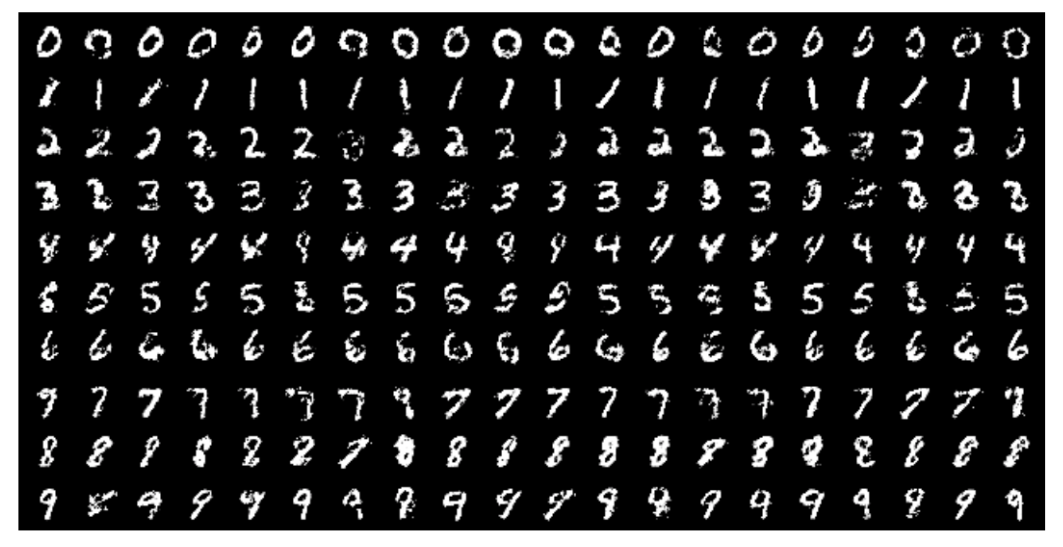
\includegraphics[width=8cm]{images/CGAN_number.jpg}
                \caption{CGAN数字生成图}
                \label{fig:CGAN数字生成图}
                \end{figure}
        % \textcolor[rgb]{1 0 0}{todo:图片:CGAN数字生成图}

    \subsection{InfoGAN}
        \subsubsection{InfoGAN模型建立}
            \par
            前面GAN生成器为$x = G(z)$,CGAN的生成器为$x = G(z,y)$,这里的$y$为指导信息。现在,考虑在生成器G的输入层加入一些$x$自身的信息,比如$x$的主成分。构建如下生成器
            \begin{align*}
            x = G(z,x')
            \end{align*}
            其中:$x'$为图像$x$的部分特征信息,例如,要生成$n\times n$大小的图像,可以用$m\times m(m <n)$的部分图像作为$x'$。进一步考虑条件GAN,有
            \begin{align*}
            x = G(z,x',y)
            \end{align*}
            其中:$x'$为$x$的部分特征,$y$为指导信息,$z$为噪声。其实,可以将$y$视为$x$的部分特征$x'$的一部分。
            \par
            现在,来看InfoGAN\cite{2017.Chen}的思路:InfoGAN将输入改为$z$和$c$。$z$仍为噪声,$c$设定为潜变量($c$可以对应于笔画粗细、图像光照、字体倾斜度等,我们称之为latent code)。设共有$L$个潜变量$c_1,c_2,\dots,c_L$(用$c$表示),于是生成器G为
            \begin{align*}
            x = G(z,c)
            \end{align*}
            并且假设$c_1,c_2,\dots,c_L$之间相互独立,即$P(c_1,c_2,\dots,c_L) = \prod_{i=1}^LP(c_i)$。生成器G构建完成之后,要考虑判别器D,D的设置仍然和前面一样。下面就要考虑如何构建目标,以及$c\sim P_c$是什么,如果$c$是$x'$或者$c$是$x$的主成分那还好说,但如果$c$是潜在的变量,那么$P_c$如何,以及如何采样$c\sim P_c$?
            \par
            如果将$x'$作为部分的输入,我们自然希望$G(z,x')$和$x'$尽可能靠近,如果把$c$视为$x'$,这里我们希望$c$和$x = G(c,z)$尽可能靠近。用互信息$I(c;x)$来衡量二者的相关性,当$c,x$相互独立时,$I(c;x) = 0$。
            \begin{align*}
            I(c;x) = I(c;G(z,c)) = H(c) - H(x|c) = H(x) -H(c|x)
            \end{align*}
            其中:$H$为熵
            \begin{align*}
            H(x) & = -\int p(x)\log p(x)\mathrm{d}x\\
            & =-\sum_{i=1}^n p_i \log p_i\\
            & =\mathbb{E}[-\log p_i]
            \end{align*}
            并且,对于互信息$I(c;x)$,我们有
            \begin{align*}
            I(c;x) &= H(c) - H(c|x)\\
            &=H(c)+H(x) - H(c,x)\\
            &=\sum_c p(c) \log \frac{1}{p(c)} + \sum _x p(x)\log \frac{1}{p(x)} - \sum_{x,c}p(c,x)\log \frac{1}{p(c,x)}\\
            &=\sum_{c,x}p(c,x) \log \frac{p(c,x)}{p(c)p(x)}
            \end{align*}
            \par
            在设置生成器G时,应该使$c$和$x = G(c,z)$的互信息$I$尽可能大,于是有InfoGAN的目标
            \begin{align*}
            \min_G\ \max_D\ V_I(D,G) = V(D,G)-\Lambda I(c;G(z,c))
            \end{align*}
            其中:$V(D,G)$是GAN的原始目标。我们来看$I(c;x)$
            \begin{align*}
            I(c;x) =&  H(c) - H(c|x)\\
            =& H(c) - \int p(c|x)\log \frac{1}{p(c|x)}\mathrm{d}x
            \end{align*}
            这样,在计算$I(c;x)$时,就需要计算后验$p(c|x)$,这是相当麻烦的。幸运的是,我们可以用$p(c|x)$的一个近似$q(c|x)$来得到$I(c;x)$的一个下界
            \begin{align*}
            I(c;x) &= H(c) - H(c|x)\\
            &=\mathbb{E}_{x\sim G(z,c)} \left [ \mathbb{E}_{c'\sim p(c|x)}[\log p(c';x)]\right] + H(c)\\
            &=\mathbb{E}_{x\sim G(z,c)}\left[ KL(P(\cdot|x)||Q(\cdot|x))+\mathbb{E}_{c'\sim p(c|x)}[\log q(c'|x)] \right]+H(c)\\
            &\geqslant\mathbb{E}_{x\sim G(z,c)} \left[\mathbb{E}_{c'\sim p(c|x)}[\log q(c'|x)]  \right]+H(c)
            \end{align*}
            \par
            上述求互信息$I$的下界的方法称为最大变分互信息(variational Information Maximization)。$H(c)$是易于计算的,在下面的分析中,我们将其视为一个常数(熵不变)。
            \par
            So far we habe by passed the problem of having to computer the posterior $p(c|x)$. explicithy wia this hower bound but we still need to be able to sample from the posterior in the inner expection.
            \begin{lemma}[lemma 5.1]
            设$X,Y$为随机变量,$f(x,y)$为二元函数,则有
            \begin{align*}
            \mathbb{E}_{x\sim X,y\sim Y|x}[f(x,y)] = \mathbb{E}_{x\sim X,y\sim Y|x,x'\sim X|y}[f(x',y)]
            \end{align*}
            \end{lemma}
            \begin{Proof}
            \begin{align*}
            \mathbb{E}_{x\sim X,y\sim Y|x}[f(x,y)] &=\int_xp(x)\int_yp(y|x)f(x,y)\mathrm{d}y\mathrm{d}x\\
            &=\iint_{x,y}p(x,y)f(x,y)\mathrm{d}y\mathrm{d}x\\
            &=\iint_{x,y}p(x,y)f(x,y)\int_{x'}p(x'|y)\mathrm{d}x'\mathrm{d}y\mathrm{d}x\\
            &=\int_x p(x)\int_y p(y|x)\int_{x'}p(x'|y)f(x',y)\mathrm{d}x'\mathrm{d}y\mathrm{d}x\\
            &=\mathbb{E}_{x\sim X,y\sim Y|x,x'\sim X|y}[f(x',y)]
            \end{align*}
            \end{Proof}
            \par
            应用上面的引理,我们可以得到互信息$I(c;x)$的一个下界
            \begin{align*}
            I(c;x) &= \mathbb{E}_{x\sim G(z,c)} \left[ \mathbb{E}_{c'\sim p(c|x)}[\log q(c'|x)] \right]+H(c)\\
            &=\mathbb{E}_{c\sim p(c),x\sim G(z,c)}[\log q(c|x)]+H(c)\\
            &\triangleq L_1(G,q)
            \end{align*}
            \par
            $L_1(G,q)$是可以用MC方法来近似(模拟)的。现在,我们将目标$L_1(G,q)$添加到GAN的目标中,求G使$L_1(G,q)$尽可能大,有
            \begin{align*}
            \min_{G,q} \ \max_D\ V_{infoGAN}(G,G,q) = V(D,G) - \lambda L_1(G,q)
            \end{align*}
        \subsubsection{InfoGAN程序}
            \par
            InfoGAN的TensorFlow程序如下
            \begin{lstlisting}[language = Python]
            import tensorflow as tf
            from tensorflow.examples.tutorials.mnist import input_data
            import numpy as np
            import matplotlib.pyplot as plt
            import matplotlib.gridspec as gridspec
            import os
            def xavier_init(size):
                in_dim = size[0]
                xavier_stddev = 1. / tf.sqrt(in_dim / 2.)
                return tf.random_normal(shape=size, stddev=xavier_stddev)
            X = tf.placeholder(tf.float32, shape=[None, 784])
            D_W1 = tf.Variable(xavier_init([784, 128]))
            D_b1 = tf.Variable(tf.zeros(shape=[128]))
            D_W2 = tf.Variable(xavier_init([128, 1]))
            D_b2 = tf.Variable(tf.zeros(shape=[1]))
            theta_D = [D_W1, D_W2, D_b1, D_b2]
            Z = tf.placeholder(tf.float32, shape=[None, 16])
            c = tf.placeholder(tf.float32, shape=[None, 10])
            G_W1 = tf.Variable(xavier_init([26, 256]))
            G_b1 = tf.Variable(tf.zeros(shape=[256]))
            G_W2 = tf.Variable(xavier_init([256, 784]))
            G_b2 = tf.Variable(tf.zeros(shape=[784]))
            theta_G = [G_W1, G_W2, G_b1, G_b2]
            Q_W1 = tf.Variable(xavier_init([784, 128]))
            Q_b1 = tf.Variable(tf.zeros(shape=[128]))
            Q_W2 = tf.Variable(xavier_init([128, 10]))
            Q_b2 = tf.Variable(tf.zeros(shape=[10]))
            theta_Q = [Q_W1, Q_W2, Q_b1, Q_b2]
            def sample_Z(m, n):
                return np.random.uniform(-1., 1., size=[m, n])
            def sample_c(m):
                return np.random.multinomial(1, 10*[0.1], size=m)
            def generator(z, c):
                inputs = tf.concat(axis=1, values=[z, c])
                G_h1 = tf.nn.relu(tf.matmul(inputs, G_W1) + G_b1)
                G_log_prob = tf.matmul(G_h1, G_W2) + G_b2
                G_prob = tf.nn.sigmoid(G_log_prob)
                return G_prob
            def discriminator(x):
                D_h1 = tf.nn.relu(tf.matmul(x, D_W1) + D_b1)
                D_logit = tf.matmul(D_h1, D_W2) + D_b2
                D_prob = tf.nn.sigmoid(D_logit)
                return D_prob
            def Q(x):
                Q_h1 = tf.nn.relu(tf.matmul(x, Q_W1) + Q_b1)
                Q_prob = tf.nn.softmax(tf.matmul(Q_h1, Q_W2) + Q_b2)
                return Q_prob
            def plot(samples):
                fig = plt.figure(figsize=(4, 4))
                gs = gridspec.GridSpec(4, 4)
                gs.update(wspace=0.05, hspace=0.05)
                for i, sample in enumerate(samples):
                    ax = plt.subplot(gs[i])
                    plt.axis('off')
                    ax.set_xticklabels([])
                    ax.set_yticklabels([])
                    ax.set_aspect('equal')
                    plt.imshow(sample.reshape(28, 28), cmap='Greys_r')
                return fig
            G_sample = generator(Z, c)
            D_real = discriminator(X)
            D_fake = discriminator(G_sample)
            Q_c_given_x = Q(G_sample)
            D_loss = -tf.reduce_mean(tf.log(D_real + 1e-8) + tf.log(1 - D_fake + 1e-8))
            G_loss = -tf.reduce_mean(tf.log(D_fake + 1e-8))
            cross_ent = tf.reduce_mean(-tf.reduce_sum(tf.log(Q_c_given_x + 1e-8) * c, 1))
            ent = tf.reduce_mean(-tf.reduce_sum(tf.log(c + 1e-8) * c, 1))
            Q_loss = cross_ent + ent
            D_solver = tf.train.AdamOptimizer().minimize(D_loss, var_list=theta_D)
            G_solver = tf.train.AdamOptimizer().minimize(G_loss, var_list=theta_G)
            Q_solver = tf.train.AdamOptimizer().minimize(Q_loss, var_list=theta_G + theta_Q)
            mb_size = 32
            Z_dim = 16
            mnist = input_data.read_data_sets('../../MNIST_data', one_hot=True)
            sess = tf.Session()
            sess.run(tf.global_variables_initializer())
            if not os.path.exists('out/'):
                os.makedirs('out/')
            i = 0
            for it in range(1000000):
                if it % 1000 == 0:
                    Z_noise = sample_Z(16, Z_dim)
                    idx = np.random.randint(0, 10)
                    c_noise = np.zeros([16, 10])
                    c_noise[range(16), idx] = 1
                    samples = sess.run(G_sample, feed_dict={Z: Z_noise, c: c_noise})
                    fig = plot(samples)
                    plt.savefig('out/{}.png'.format(str(i).zfill(3)), bbox_inches='tight')
                    i += 1
                    plt.close(fig)
                X_mb, _ = mnist.train.next_batch(mb_size)
                Z_noise = sample_Z(mb_size, Z_dim)
                c_noise = sample_c(mb_size)
                _, D_loss_curr = sess.run([D_solver, D_loss],
                                          feed_dict={X: X_mb, Z: Z_noise, c: c_noise})
                _, G_loss_curr = sess.run([G_solver, G_loss],
                                          feed_dict={Z: Z_noise, c: c_noise})
                sess.run([Q_solver], feed_dict={Z: Z_noise, c: c_noise})
                if it % 1000 == 0:
                    print('Iter: {}'.format(it))
                    print('D loss: {:.4}'. format(D_loss_curr))
                    print('G_loss: {:.4}'.format(G_loss_curr))
            print()
            \end{lstlisting}
            \par
            在实验中,作者通过只改变latent code c中的某一个维度,来观察生成数据的变化。其实验确实证明:latent code确实学到了一些维度,如图像的角度或光照等因素,也即说明InfoGAN确实学习到了数据中的disentangled的可解释部分的表示。其效果如下三张图(\ref{fig:infoGAN实验结果})所示
                \begin{figure}[H]
                \centering
                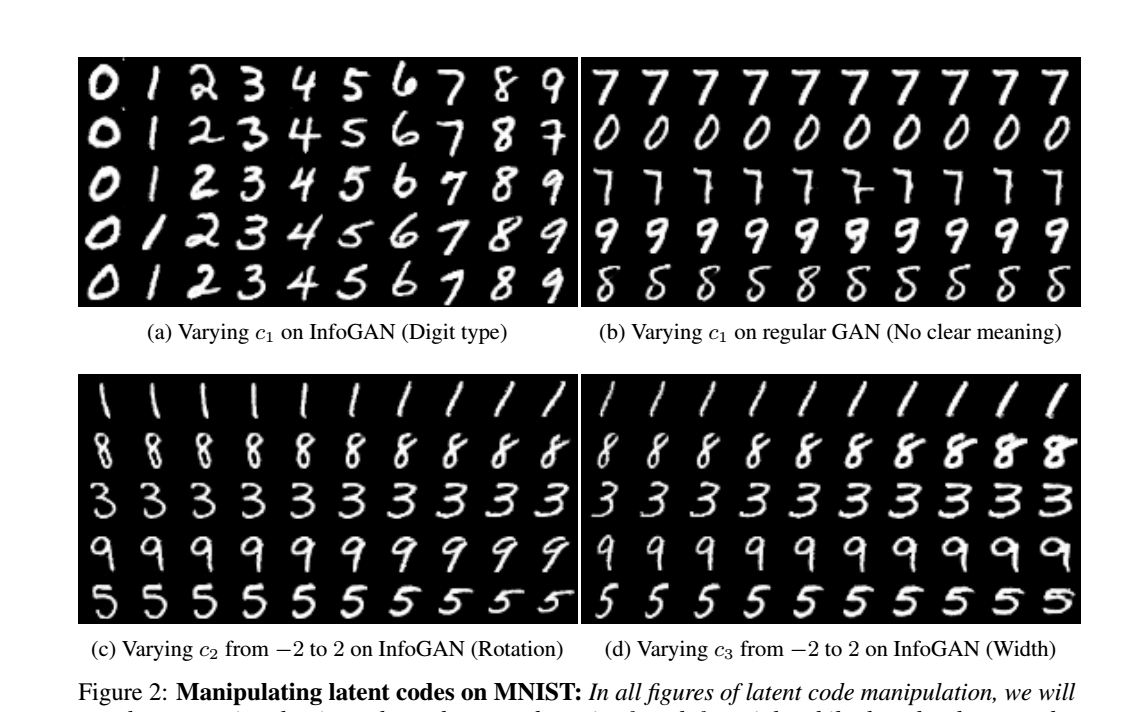
\includegraphics[width=7cm]{images/InfoGAN1}
                \qquad
                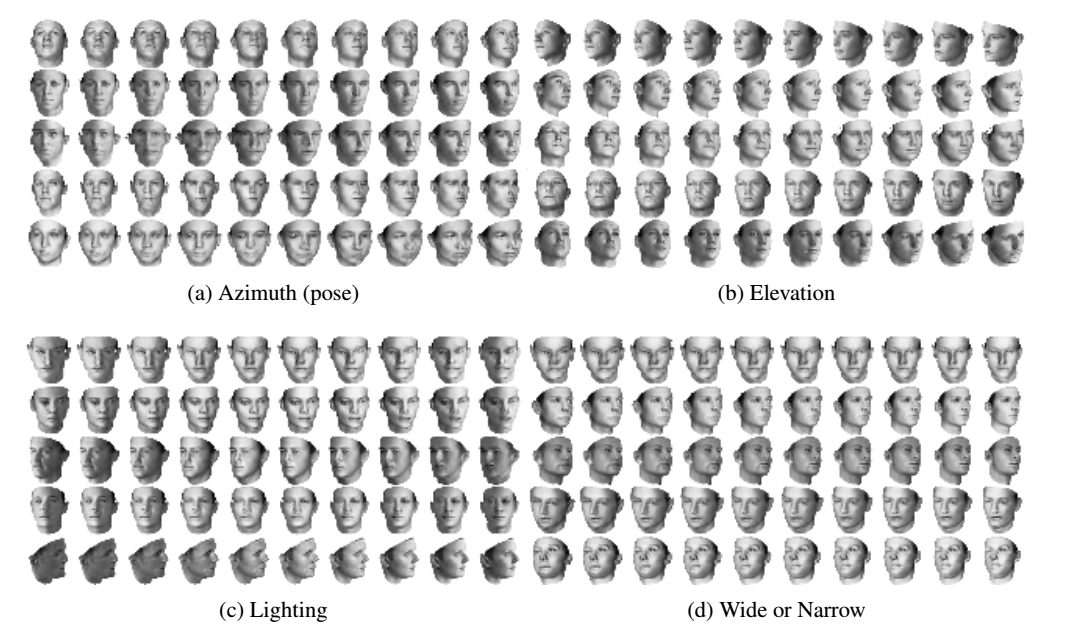
\includegraphics[width=7cm]{images/InfoGAN2}
                \qquad
                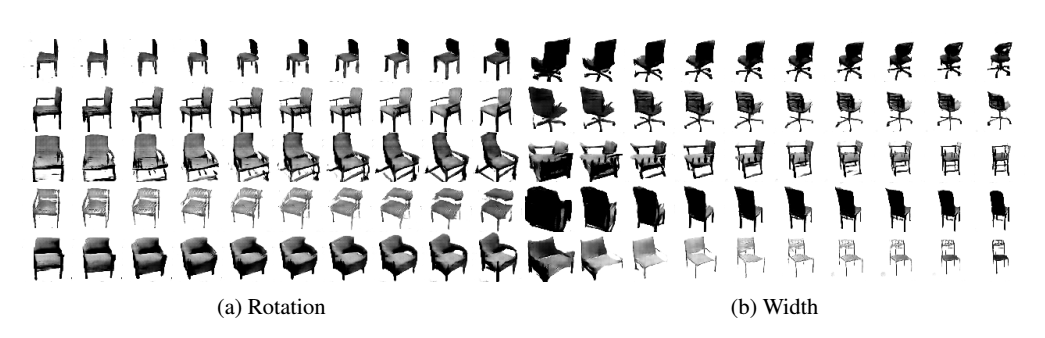
\includegraphics[width=10cm]{images/InfoGAN3}
                \caption{infoGAN实验结果}
                \label{fig:infoGAN实验结果}
                \end{figure}
            % \textcolor[rgb]{1 0 0}{todo:图片:InfoGAN效果图}

    \subsection{Mali GAN}
        \subsubsection{Mali GAN模型建立}
            \par
            尽管生成对抗网络(GAN)在获取连续分布上已经取得了成功,但其在离散背景(比如自然语言任务)上的应用却相当有限。主要的原因是通过离散变量的反向传播很困难,而且 GAN 训练目标还具有固有的不稳定性。为了解决这些问题,文献\cite{2017.Tong}提出了最大似然增强的离散生成对抗网络(Maximum-Likelihood Augmented Discrete Generative Adversarial Networks)。Mali GAN没有直接优化该 GAN 目标,而是使用遵循对数似然的推导提出了一种全新的且低方差的目标。在多种离散数据集上的实验结果表明了这方法的有效性。
            \par
            在GAN的分析中,我们知道在G给定的情况下,最优判别器D为
            \begin{align*}
            D^* = \frac{p_r}{p_r+p_g}
            \end{align*}
            给定$D^*$,真实分布密度$p_r$可以写为
            \begin{align*}
            p_r(x) = \frac{D^*}{1-D^*}p_g(x)
            \end{align*}
            即真实样本的概率可以用$p_g$的带权$\frac{D^*}{1-D^*}$来替代。然而,这样的判别器D不太可能通过训练得到,甚至不存在。为此,我们将最优$D^*$改为非最优判别器$D(x)$,据此,我们可以写出,在D给定下$p_r$的估计
            \begin{align*}
            \tilde{p}_r = \frac{D}{1-D}p_g
            \end{align*}
            上式说明,在D和G给定下,样本$x$在真实分布$p_r$中的估计值。\ding{172}回想极大似然估计,我们的目标是让样本出现的概率最大。现在可以求G,让G生成的假样本在真实分布$p_r$中的概率值最大,即
            \begin{align*}
            \max_G\  \tilde{p}_r(x)
            \end{align*}
            \par
            \ding{173}在GAN中,生成器G的目标是使两个分布$p_r,p_g$的JSD散度最小。这里,将JSD散度换为KL距离,有
            \begin{align*}
            \min_G \ KL(p_r||p_g)
            \end{align*}
            用$\tilde{p}_r$来替代$p_r$,有
            \begin{align*}
            \min_G \ KL(\tilde{p}_r||p_g)
            \end{align*}
            \par
            但可惜的是$\tilde{p}_r$并不是一个合理的概率分布,因为它的和并不为1。为此,使用归一化技术,令$r_D(x) = \frac{D(x)}{1-D(x)}$,定义归一化的$p_r$的估计为
            \begin{align*}
            q(x) = \frac{1}{Z(\theta')} \frac{D(x)}{1-D(x)} p_g(x) = \frac{r_D(x)}{Z(\theta')}p_g(x)
            \end{align*}
            其中:$Z(\theta')$为归一化因子,$Z(\theta') = \mathbb{E}_{p_g}[r_D(x)] = \sum_x p_g(x) \frac{D(x)}{1-D(x)}$。此时的$q(x)$是一个标准的概率分布,其和为1。当最优判别器是$D = D^* = \frac{1}{2}$时,$Z = 1$,$q(x) = p_g(x) = p_r(x)$,并且$q(x)$估计量的偏差仅依赖于$D(x)$,$D^*(x) = D(x)$是最小偏差。
            \par
            我们的目标是求G使$p_g$和$q$的KL距离最小(用$q$来代替$p_r$)
            \begin{align*}
            L_G(\theta_g) = KL(q(x)||p_{\theta_g}(x))
            \end{align*}
            上述目标有一个吸引人的性质:$q$是固定的。如果D被充分训练,则$q$总是接近数据分布$p_r$。定义目标的导数为$\nabla L_G = \mathbb{E}_q[\nabla_{\theta_g} \log p_{\theta_g}(x)]$,有
            \begin{align*}
            \nabla L_G =& \mathbb{E}_{p_g} \left[ \frac{q(x)}{p_g(x)} \nabla_{\theta_g}\log p_{\theta_g}(x) \right]\\
            =& \frac{1}{Z}\mathbb{E}_{p_{\theta_g}} \left[r_D(x) \nabla_{\theta_g}\log p_{\theta_g}(x) \right]
            \end{align*}
            \par
            Mali GAN通过如下的梯度估计量来求解G
            \begin{align}
            \label{近似目标}
            \nabla L_G(\theta_g) \approx \sum_{i=1}^m \left( \frac{r_D(x_i)}{\sum_i r_D(x_i)} - b \right) \nabla \log p_{\theta_g}(x_i) = \mathbb{E}(\{x_i\})
            \end{align}
            其中:$b$是一个baseline,用来增强学习以减小方差。在试验中,让$b$从0到1慢慢变大。下面,给出这种梯度近似的合理性。下述定理表明,当D接近最优时,上面的近似目标(\ref{近似目标})接近原始目标$KL(q(x)||p_g(x))$。此外,即使D没有接近最优,这个近似目标(\ref{近似目标})仍然是很好的。
            \begin{theorem}
            \par
            1.如果$D(x)$是最优的,有如下等式
            \begin{align*}
            \mathbb{E}_{p_r}[\log p_{\theta_d}(x)] = \frac{1}{Z(\theta')} \mathbb{E}_{p_g}[r_D(x)\log p_{\theta_g}(x)]
            \end{align*}
            其中:$Z(\theta') = \mathbb{E}_{p_g}[r_D(x)]$。
            \par
            2.如果$D(x)$被训练的很好,但不是最优,$\forall x$,$D(x)$在0.5到$\frac{p_r}{p_r+p_g}$,我们有:当$m\to\infty$时,almost surely
            \begin{align*}
            \mathbb{E}(\{x_i\}_{i=1}^m)\nabla _\theta KL(p_r||p_{\theta_g}) > 0
            \end{align*}
            \end{theorem}
        \subsubsection{Mali GAN算法}
            \par
            Mali GAN的伪代码如(\ref{code:Mali GAN})所示
            \begin{algorithm}[H]
                \caption{Minibatch stochastic gradient descent training of Mali GAN}\label{code:Mali GAN}
                \begin{algorithmic}[1]
                    \State 初始化:一个含参数$\theta_g$的生成器$p_{\theta_g}$;一个含参数$\theta_d$的判别器$D(x)$;baseline $b$;迭代数$t$,$t_{max}$;判别器训练次数$k$;批量大小$m$。
                    \For {$t=1,2,\dots,t_{max}$}
                        \State $//$更新D
                        \For {$k$ steps}
                            \State sample minibatch of m noise sample $\{z^{(1)},z^{(2)},\dots,z^{(m)}\}$ from $P_z$;生成$m$个假样本$x^{(1)} = G(z^{(1)}),x^{(2)} = G(z^{(2)}),\dots,x^{(m)} = G(z^{(m)})$。
                            \State sample minibatch of m example $\{x^{(1)},x^{(2)},\dots,x^{(m)}\}$ from $P_r$,即从原始数据$\{x_i\}_{i=1}^n$中挑出$m$个。
                            \State 求D的梯度
                            \begin{align*}
                            \nabla_{\theta_d} \frac{1}{m} \sum_{i=1}^m [\log D_t(x^{(i)})+\log (1-D_t(G_t(z^{(i)})))]
                            \end{align*}
                            \State 求$D_{t+1} = D_t+\nabla_{\theta_d}$;
                        \EndFor
                        \State $//$ 更新G
                        \State sample minibatch of m noise sample $\{z^{(1)},z^{(2)},\dots,z^{(m)}\}$ from $P_z$;
                        \State 计算梯度
                        \begin{align*}
                        \sum_{i=1}^m \left( \frac{r_D(G(z^{(i)}))}{\sum_i r_D(G(z^{(i)}))} - b \right) \nabla \log p_{\theta_g}(G(z^{(i)}))
                        \end{align*}
                        \State 更新$G$
                        \begin{align*}
                        G_{t+1} = G_t + \nabla_{\theta_g}
                        \end{align*}
                    \EndFor
                \end{algorithmic}
            \end{algorithm}

    \subsection{Boundary Seeking GAN}
        \subsubsection{BGAN模型建立}
            \par
            在Mali GAN中,当$p_g(x)$已知时,在$D(x)$给定后,就可以得到$p_r$的近似$\tilde{p_r}$和$q$。并且
            \begin{align*}
            p_g(x) & = \sum_z g(x|z)p(z)\\
            & =\int_zg(x,z)\mathrm{d}z\\
            & =\int_z g(x|z)p(z)\mathrm{d}z
            \end{align*}
            G的目标是使$q$和$p_g$的KL距离最小
            \begin{align*}
            \min_G \ KL(q(x)||p_g(x))
            \end{align*}
            设$G$的参数为$\theta_g$,有
            \begin{align*}
            &\nabla_{\theta_g} KL(q(x)||p_g(x))\\
            ={}&\nabla_{\theta_g} \sum_x q(x)\log \frac{q(x)}{p_g(x)}\\
            \approx{}&-\sum_x q(x)\nabla_{\theta_g}\log p_g(x)\\
            ={}&-\sum_x \frac{1}{Z}p_g(x)\frac{D(x)}{1-D(x)} \nabla_{\theta_g}\log p_g(x)\\
            ={}&-\sum_x \frac{1}{Z}\sum_z g(x|z)p(z)\frac{D(x)}{1-D(x)}\nabla_{\theta_g}\log p_g(x)
            \end{align*}
            其中:$Z$是归一化因子,$Z = \sum _x p_g(x)\frac{D(x)}{1-D(x)}$
            \par
            上面这个梯度$\nabla_{\theta_g}$需要用MC等方法近似,并且会有很大的方差,尤其在解决$Z$时。The intuition here is to note that, as the conditional density,$ g(x|z)$ is unimodal(单峰的),$g(x|z)$可以用来构建一个和$q(x)$类似的分布
            \begin{align*}
            \tilde{p}_z = \frac{1}{Z_z} g(x|z) \frac{D(x)}{1-D(x)}
            \end{align*}
            其中:我们使用了$\log p_g(x) = \log g(x|z) + \log p(z)$,$Z_z = \sum_x g(x|z) \frac{D(x)}{1-D(x)}$是边缘,确保$\tilde{p}_z$是一个概率分布。The gradients then become
            \begin{align*}
            \nabla_{\theta_g} KL(\tilde{p}_z(x)||g(x|z)) \approx& -\sum _x\tilde{p}_z(x) \nabla_{\theta_g(x|z)}\\
            \approx& -\sum_m \tilde{w}^{(m)} \nabla_{\theta_g}\log g(x^{(m)}|z)
            \end{align*}
            其中:$\tilde{w}^{(m)} = \frac{w^{(m)}}{\sum_{m'}w^{(m')}}$和$w^{(m)} = \frac{D(x^{(m)})}{1-D(x^{(m)})}$分别是归一化和非归一化权重;$x^{(m)}$是给定$z$后生成器生成的样本。当从$D(x)$角度看样本是相当糟糕时,即$w^{(m)}$很大或很小时,归一化是有帮助的。
            \par
            $\theta_g$可以采用批量样本来更新
            \begin{align*}
            \nabla_{\theta_g} \propto \frac{1}{N} \sum_n\sum _m \tilde{w}^{(m)} \nabla_{\theta_g} \log g(x^{(m)}|z^{(m)})
            \end{align*}

        \subsubsection{BGAN程序}
            \par
            Boundary Seeking GAN的TensorFolw程序如下
            \begin{lstlisting}[language = Python]
            import tensorflow as tf
            from tensorflow.examples.tutorials.mnist import input_data
            import numpy as np
            import matplotlib.pyplot as plt
            import matplotlib.gridspec as gridspec
            import os
            mb_size = 32
            X_dim = 784
            z_dim = 64
            h_dim = 128
            lr = 1e-3
            d_steps = 3
            mnist = input_data.read_data_sets('../../MNIST_data', one_hot=True)
            def plot(samples):
                fig = plt.figure(figsize=(4, 4))
                gs = gridspec.GridSpec(4, 4)
                gs.update(wspace=0.05, hspace=0.05)
                for i, sample in enumerate(samples):
                    ax = plt.subplot(gs[i])
                    plt.axis('off')
                    ax.set_xticklabels([])
                    ax.set_yticklabels([])
                    ax.set_aspect('equal')
                    plt.imshow(sample.reshape(28, 28), cmap='Greys_r')
                return fig
            def xavier_init(size):
                in_dim = size[0]
                xavier_stddev = 1. / tf.sqrt(in_dim / 2.)
                return tf.random_normal(shape=size, stddev=xavier_stddev)
            def log(x):
                return tf.log(x + 1e-8)
            X = tf.placeholder(tf.float32, shape=[None, X_dim])
            z = tf.placeholder(tf.float32, shape=[None, z_dim])
            D_W1 = tf.Variable(xavier_init([X_dim, h_dim]))
            D_b1 = tf.Variable(tf.zeros(shape=[h_dim]))
            D_W2 = tf.Variable(xavier_init([h_dim, 1]))
            D_b2 = tf.Variable(tf.zeros(shape=[1]))
            G_W1 = tf.Variable(xavier_init([z_dim, h_dim]))
            G_b1 = tf.Variable(tf.zeros(shape=[h_dim]))
            G_W2 = tf.Variable(xavier_init([h_dim, X_dim]))
            G_b2 = tf.Variable(tf.zeros(shape=[X_dim]))
            theta_G = [G_W1, G_W2, G_b1, G_b2]
            theta_D = [D_W1, D_W2, D_b1, D_b2]
            def sample_z(m, n):
                return np.random.uniform(-1., 1., size=[m, n])
            def generator(z):
                G_h1 = tf.nn.relu(tf.matmul(z, G_W1) + G_b1)
                G_log_prob = tf.matmul(G_h1, G_W2) + G_b2
                G_prob = tf.nn.sigmoid(G_log_prob)
                return G_prob
            def discriminator(x):
                D_h1 = tf.nn.relu(tf.matmul(x, D_W1) + D_b1)
                out = tf.nn.sigmoid(tf.matmul(D_h1, D_W2) + D_b2)
                return out
            G_sample = generator(z)
            D_real = discriminator(X)
            D_fake = discriminator(G_sample)
            D_loss = -tf.reduce_mean(log(D_real) + log(1 - D_fake))
            G_loss = 0.5 * tf.reduce_mean((log(D_fake) - log(1 - D_fake))**2)
            D_solver = (tf.train.AdamOptimizer(learning_rate=lr)
                        .minimize(D_loss, var_list=theta_D))
            G_solver = (tf.train.AdamOptimizer(learning_rate=lr)
                        .minimize(G_loss, var_list=theta_G))
            sess = tf.Session()
            sess.run(tf.global_variables_initializer())
            if not os.path.exists('out/'):
                os.makedirs('out/')
            i = 0
            for it in range(1000000):
                X_mb, _ = mnist.train.next_batch(mb_size)
                z_mb = sample_z(mb_size, z_dim)
                _, D_loss_curr = sess.run(
                    [D_solver, D_loss],
                    feed_dict={X: X_mb, z: z_mb}
                )
                _, G_loss_curr = sess.run(
                    [G_solver, G_loss],
                    feed_dict={X: X_mb, z: sample_z(mb_size, z_dim)}
                )
                if it % 1000 == 0:
                    print('Iter: {}; D_loss: {:.4}; G_loss: {:.4}'
                          .format(it, D_loss_curr, G_loss_curr))
                    samples = sess.run(G_sample, feed_dict={z: sample_z(16, z_dim)})
                    fig = plot(samples)
                    plt.savefig('out/{}.png'
                                .format(str(i).zfill(3)), bbox_inches='tight')
                    i += 1
            plt.close(fig)
            \end{lstlisting}

    \subsection{Mode Regularized GAN}
        \subsubsection{MRGAN模型建立}
            \par
            GAN在许多任务上都表现良好,但GAN有两大缺点:1.训练极不稳定;2.生成的图片多样性较差。和无监督GAN相比,有监督CGAN的训练要相对稳定一些。而CGAN相对GAN而言,其目标中多了一个$I(c;G(z,c))$,也就是说,就是此项让GAN变得稳定了一些。而此项可以被视为一个正则项,我们自然考虑其他的正则方法,文献\cite{2016.Tong}就考虑了一些正则化GAN。
            \par
            假设生成器G是$G(z):Z\to X$的映射,相应的,我们考虑一个encoder $E(x):X\to Z$。并且假设$d$是某一种相似性度量,$p_r$是真实分布,$p_g$是生成分布。我们使用$\mathbb{E}_{x\sim p_r}[d(x,G\circ E(x)]$作为正则项,其中$G\circ E$是一个自动编码器。for $x\in M_0$,如果$G\circ E$是一个好的自动编码器,则$G\circ E$应该和$M_0$非常接近。在训练G时,添加正则项$\mathbb{E}_{x\sim p_r}[d(x,G\circ E(x)]$
            \begin{align*}
            & T_G = -\mathbb{E}_{z\sim p_z}[\log D(G(z))] +\mathbb{E}_{x\sim p_r}[\lambda_1 d(x,G\circ E(x))+\lambda_2\log D(G\circ E(x))]\\
            & T_E = \mathbb{E}_{x\sim p_r}[\lambda_1d(x,G\circ E(x))+ \lambda_2\log D(G\circ E(x))]
            \end{align*}
            \par
            The proposed algorithm divides the training procedure of GANs into two steps: a manifold step and a diffusion step. In the manifold step, we try to match the generation manifold and the real data manifold with the help of an encoder and the geometric metric loss. In the diffusion step, we try to distribute the probability mass on the generation manifold fairly according to the real data distribution.

        \subsubsection{MRGAN程序}
            \par
            MRGAN的伪代码如(\ref{code:MRGAN})所示
            \begin{algorithm}[htbp]
                \caption{Minibatch stochastic gradient descent training of MRGAN}\label{code:MRGAN}
                \begin{algorithmic}[1]
                    \State \textbf{Manifold Step:}。
                    \State 从真实分布$p_r$中抽取$m$个样本$\{x_1,x_2,\dots,x_m\}$。
                    \State 使用SGD来更新判别器$D_1$
                    \begin{align*}
                    \nabla_{\theta_d^1} \frac{1}{m} \sum_{i=1}^m [\log D_1(x_i)+\log (1-D_1(G(E(x_i))))]
                    \end{align*}
                    \State 使用SGD来更新生成器G
                    \begin{align*}
                    \nabla _{\theta_g} \frac{1}{m}\sum_{i=1}^m [\lambda\log D_1(G(E(x_i))) - ||x_i - G(E(x_i))||^2]
                    \end{align*}
                    \State \textbf{Diffusion Step:}
                    \State 从真实分布$p_r$中抽取$m$个样本$\{x_1,x_2,\dots,x_m\}$。
                    \State 从prior 分布$p_z$中抽取$m$个样本$\{z_1,z_2,\dots,z_m\}$。
                    \State 使用SGD更新判别器$D_2$
                    \begin{align*}
                    \nabla_{\theta_d^2}\frac{1}{m}\sum_{i=1}^m [\log D_2(G(E(x_i)))+\log (1-D_2(z_i))]
                    \end{align*}
                    \State 使用SGD来更新生成器G
                    \begin{align*}
                    \nabla_{\theta_g} \frac{1}{m}\sum_{i=1}^m[\log D_2(G(z_i))]
                    \end{align*}
                \end{algorithmic}
            \end{algorithm}
            \par
            MRGAN的pytorch程序如下
            \begin{lstlisting}[language = Python]
            import torch
            import torch.nn
            import torch.nn.functional as nn
            import torch.autograd as autograd
            import torch.optim as optim
            import numpy as np
            import matplotlib.pyplot as plt
            import matplotlib.gridspec as gridspec
            import os
            from torch.autograd import Variable
            from tensorflow.examples.tutorials.mnist import input_data
            mnist = input_data.read_data_sets('../../MNIST_data', one_hot=True)
            mb_size = 32
            z_dim = 128
            X_dim = mnist.train.images.shape[1]
            y_dim = mnist.train.labels.shape[1]
            h_dim = 128
            cnt = 0
            lr = 1e-4
            lam1 = 1e-2
            lam2 = 1e-2
            def log(x):
                return torch.log(x + 1e-8)
            E = torch.nn.Sequential(
                torch.nn.Linear(X_dim, h_dim),
                torch.nn.ReLU(),
                torch.nn.Linear(h_dim, z_dim)
            )
            G = torch.nn.Sequential(
                torch.nn.Linear(z_dim, h_dim),
                torch.nn.ReLU(),
                torch.nn.Linear(h_dim, X_dim),
                torch.nn.Sigmoid()
            )
            D = torch.nn.Sequential(
                torch.nn.Linear(X_dim, h_dim),
                torch.nn.ReLU(),
                torch.nn.Linear(h_dim, 1),
                torch.nn.Sigmoid()
            )
            def reset_grad():
                G.zero_grad()
                D.zero_grad()
                E.zero_grad()
            def sample_X(size, include_y=False):
                X, y = mnist.train.next_batch(size)
                X = Variable(torch.from_numpy(X))
                if include_y:
                    y = np.argmax(y, axis=1).astype(np.int)
                    y = Variable(torch.from_numpy(y))
                    return X, y
                return X
            E_solver = optim.Adam(E.parameters(), lr=lr)
            G_solver = optim.Adam(G.parameters(), lr=lr)
            D_solver = optim.Adam(D.parameters(), lr=lr)
            for it in range(1000000):
                """ Discriminator """
                # Sample data
                X = sample_X(mb_size)
                z = Variable(torch.randn(mb_size, z_dim))
                # Dicriminator_1 forward-loss-backward-update
                G_sample = G(z)
                D_real = D(X)
                D_fake = D(G_sample)
                D_loss = -torch.mean(log(D_real) + log(1 - D_fake))
                D_loss.backward()
                D_solver.step()
                # Housekeeping - reset gradient
                reset_grad()
                """ Generator """
                # Sample data
                X = sample_X(mb_size)
                z = Variable(torch.randn(mb_size, z_dim))
                # Generator forward-loss-backward-update
                G_sample = G(z)
                G_sample_reg = G(E(X))
                D_fake = D(G_sample)
                D_reg = D(G_sample_reg)
                mse = torch.sum((X - G_sample_reg)**2, 1)
                reg = torch.mean(lam1 * mse + lam2 * log(D_reg))
                G_loss = -torch.mean(log(D_fake)) + reg
                G_loss.backward()
                G_solver.step()
                # Housekeeping - reset gradient
                reset_grad()
                """ Encoder """
                # Sample data
                X = sample_X(mb_size)
                z = Variable(torch.randn(mb_size, z_dim))
                G_sample_reg = G(E(X))
                D_reg = D(G_sample_reg)
                mse = torch.sum((X - G_sample_reg)**2, 1)
                E_loss = torch.mean(lam1 * mse + lam2 * log(D_reg))
                E_loss.backward()
                E_solver.step()
                # Housekeeping - reset gradient
                reset_grad()
                # Print and plot every now and then
                if it % 1000 == 0:
                    print('Iter-{}; D_loss: {}; E_loss: {}; G_loss: {}'
                          .format(it, D_loss.data.numpy(), E_loss.data.numpy(), G_loss.data.numpy()))
                    samples = G(z).data.numpy()[:16]
                    fig = plt.figure(figsize=(4, 4))
                    gs = gridspec.GridSpec(4, 4)
                    gs.update(wspace=0.05, hspace=0.05)
                    for i, sample in enumerate(samples):
                        ax = plt.subplot(gs[i])
                        plt.axis('off')
                        ax.set_xticklabels([])
                        ax.set_yticklabels([])
                        ax.set_aspect('equal')
                        plt.imshow(sample.reshape(28, 28), cmap='Greys_r')
                    if not os.path.exists('out/'):
                        os.makedirs('out/')
                    plt.savefig('out/{}.png'
                                .format(str(cnt).zfill(3)), bbox_inches='tight')
                    cnt += 1
            plt.close(fig)
            \end{lstlisting}

    \subsection{DCGAN}
        \par
        由于GAN的模型不稳定性问题比较突出,因而在2016年出现的关于GAN训练技巧的成果有许多,目前被广泛应用的主要包括:DCGAN\footnote{http://www.leiphone.com/news/201703/Y5vnDSV9uIJIQzQm.html}\footnote{https://github.com/roatienza/Deep-Learning-Experiments/blob/master/Experiments/Tensorflow/GAN/dcgan\_mnist.py} (ICLR-2016) 和Improved GAN (NIPS-2016 workshop),特别是DCGAN,几乎在各大GAN模型中都能看到它的身影。
        \par
        DCGAN\cite{2015.Radford} 的模型结构如图(\ref{fig:DCGAN网络结构图})所示所示
                \begin{figure}[H]
                \centering
                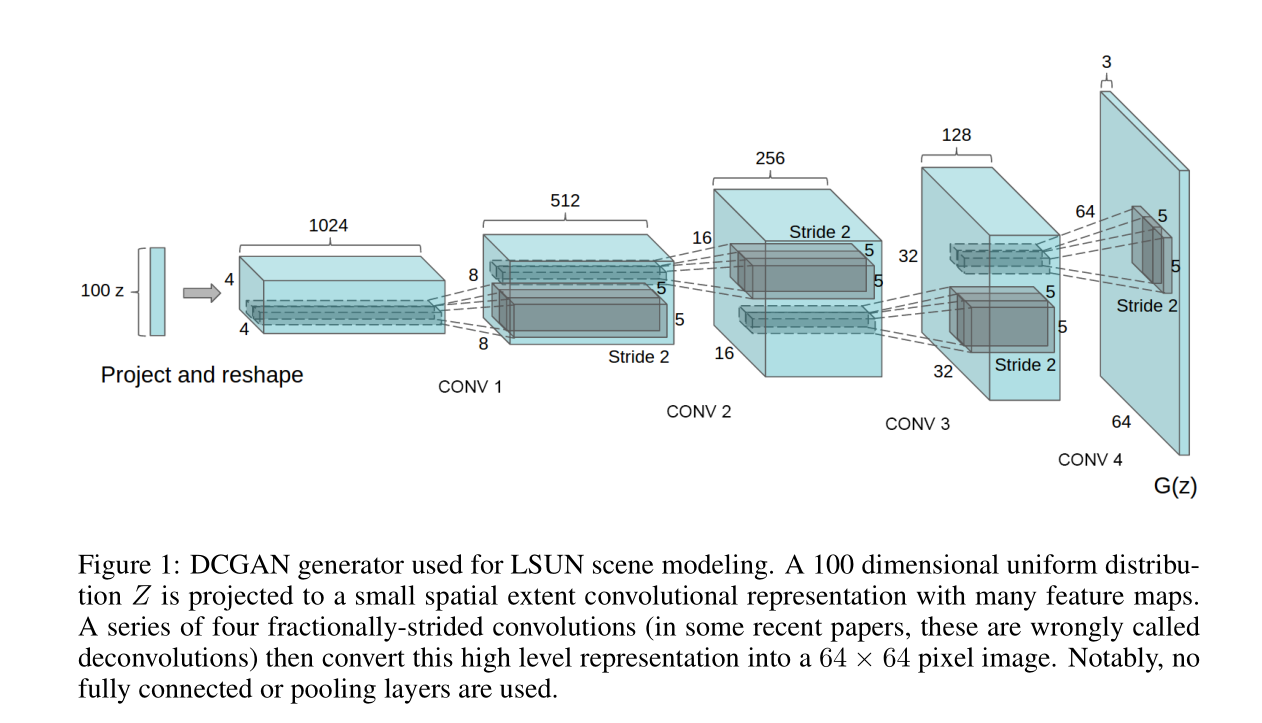
\includegraphics[width=12cm]{images/DCGAN_network.jpg}
                \caption{DCGAN网络结构图}
                \label{fig:DCGAN网络结构图}
                \end{figure}
        % \textcolor[rgb]{1 0 0}{todo:图片:DCGAN网络结构图}\\
        其输入为100维的噪声向量,经过一系列的strided conv操作,形成64$\times$64的图像,即为$G(z)$。而判别器结构与之类似,只是是由一系列的卷积操作构成 (而非strided conv),最后由average pooling形成判别器的标量输出。在DCGAN\cite{2015.Radford}中,最主要的是提出了以下四条有助于稳定训练GAN的方法:
        \begin{enumerate}
        \item 去掉max pooling操作:用strided conv代替原来的pooling操作,使网络自动学习合适的采样核函数;
        \item 去掉全连接层:用global average pooling代替全连接层;虽然该操作可能会导致收敛速度变慢,但有助于整体训练的稳定性;
        \item 加入BN层:之前的LAPGAN\cite{2015.Denton}指出,如果像常规模型一样对所有层都施加BN,则会引起GAN的模型崩溃,而DCGAN通过对generator的输出层和discriminator的输入层不用BN,而其他层都用BN,则缓解了模型崩溃问题,并且有效避免了模型的振荡和不稳定问题。
        \item 激活函数的选择:在generator中除了输出层用tanh外,其余都用RELU函数;而在discriminator中采用leaky ReLU函数。
        \end{enumerate}

    \subsection{Improved GAN}
        \par
        文献\cite{2016.Tim}主要给出了5条有助于GAN稳定训练的经验:
        \begin{enumerate}
        \item 特征匹配:让生成器产生的样本与真实样本在判别器中间层的响应一致,即使判别器从真实数据和生成数据中提取的特征一致,而不是在判别器网络的最后一层才做判断,有助于提高模型的稳定性;其实验也表明在一些常规方法训练GAN不稳定的情况中,若用特征匹配则可以有效避免这种不稳定;
        \item Minibatch Discrimination:在判别器中,不再每次对每一个生成数据与真实数据的差异性进行比较,而是一次比较一批生成数据与真实数据的差异性。这种做法提高了模型的鲁棒性,可以缓解生成器输出全部相似或相同的问题;
        \item Historical Averaging:受fictitious  play的游戏算法启发,作者提出在生成器和判别器的目标函数中各加一个对参数的约束项
        \begin{align*}
        \bigg|\bigg|\theta - \frac{1}{t}\sum_{i=1}^t\theta_t\bigg|\bigg|^2
        \end{align*}
        其中:$\theta_i$表示在时刻$i$的模型参数,该操作可以在一些情况下帮助模型达到模型的平衡点;
        \item 单边标签平滑 (One-sided Label Smoothing):当向GAN中引入标签数据时,最好是将常规的0、1取值的二值标签替换为如0.1、0.9之类的平滑标签,可以增加网络的抗干扰能力;但这里之所以说单边平滑,是因为假设生成数据为0.1而非0的话会使判别器的最优判别函数的形状发生变化,会使生成器偏向于产生相似的输出,因此对于取值0的标签保持不变,不用0.1一类的小数据替换,即为单边标签平滑;
        \item Virtual Batch Normalization:VBN相当于是BN的进阶版,BN是一次对一批数据进行归一化,这样的一个副作用是当“批”的大小不同时,BN操作之后的归一化常量会引起训练过程的波动,甚至超过输入信号$z$的影响(因$z$是随机噪声);而VBN通过引入一个参考集合,每次将当下的数据$x$加入参考集合构建一个新的虚拟的batch,然后在这个虚拟的batch上进行归一化,如此可以缓解原始BN操作所引起的波动问题。
        \end{enumerate}

    \subsection{Least Squares GAN}
        \subsubsection{LSGAN模型建立}
            \par
            在GAN中,设$D(x)\in [0,1]$为样本$x$为真的概率,作为损失,我们将其取$\log$,设定为$\log D(x)$。我们的目标是用D将G所生成的样本/分布“拖”到真实数据流(data manifold)当中(1维线二维面三维体三维以上称为流形),从而使G生成的样本类似于$p_r(x)$的样本。
            \par
            我们知道常规GAN中,判别器使用的是对数损失log loss($1-D$为损失,再取$\log$)。就简单的二分类问题而言,对数损失带来的决策边界如图(\ref{fig:LSGAN-sigmoid决策边界图})所示
                \begin{figure}[H]
                \centering
                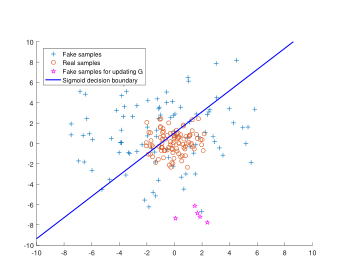
\includegraphics[width=6cm]{images/LSGAN-sigmoid.jpg}
                \caption{LSGAN-sigmoid决策边界图}
                \label{fig:LSGAN-sigmoid决策边界图}
                \end{figure}
            % \textcolor[rgb]{1 0 0}{todo:图片:LSGAN-sigmoid决策边界图-需要修改}\\
            因为D使用的是sigmoid函数,sigmoid函数饱和的十分迅速,所以即使是十分小的数据点$x$,该函数也会迅速忽略$x$到决策边界的距离。这意味着,sigmoid函数本质上不会惩罚远离决策边界的$x$,也就说明,我们满足于将样本正确分类,当$x$变得很大时,D的梯度就会快速下降为0。因此,sigmoid不关心样本点到决策边界的距离,只关心是否分类正确。而G的训练依赖于D的梯度,当D的梯度为0时,G就不再更新(GAN训练不稳定)。
            \par
            Least squares loss:就简单的二分类问题而言,最小平方损失的决策如图(\ref{fig:LSGAN-L2决策边界图})所示
                \begin{figure}[H]
                \centering
                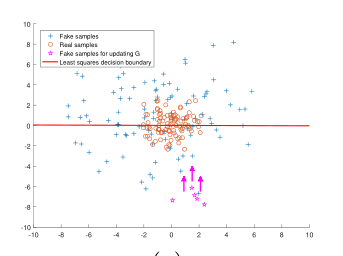
\includegraphics[width=8cm]{images/LSGAN-L2decision.jpg}
                \caption{LSGAN-L2决策边界图}
                \label{fig:LSGAN-L2决策边界图}
                \end{figure}
            在L2损失中,距$w$远的数据将会获得与距离成正比的惩罚,因此梯度只有在$w$完全拟合$x$的情况下才为0。如果G没有捕获到数据流形,那么这将能确保D服从多信息梯度(information gradients)。在优化过程中,G使D的损失减小的唯一方式是尽可能的接近W($x = G(z)$接近$w$)。
            \par
            LSGAN设置L2损失$D(x)\in [0,1]$,将真样本概率值$D(x)$的期望设置为$b$,假样本概率值$D(x)$的期望设置为$a$,有
            \begin{align*}
            & \min_D \ V(D) = \frac{1}{2} \mathbb{E}_{x\sim p_r}[(D(x) - 1)^2] + \frac{1}{2}\mathbb{E}_{z\sim p_z}p[(D(G(z))-0)^2]\\
            & \min_G \ V(G) = \frac 12 \mathbb{E}_{z\sim p_z}[(D(G(z))-1)^2]
            \end{align*}
            我们将D和G的目标进行如下扩展
            \begin{align*}
            & \min_D \ V(D) = \frac{1}{2} \mathbb{E}_{x\sim p_r}[(D(x) - b)^2] + \frac{1}{2}\mathbb{E}_{z\sim p_z}p[(D(G(z))-a)^2]\\
            & \min_G \ V(G) = \frac{1}{2} \mathbb{E}_{x\sim p_r}[(D(x) - c)^2] + \frac 12 \mathbb{E}_{z\sim p_z}[(D(G(z))-c)^2]
            \end{align*}
            并且,注意到在G的目标中添加了$\mathbb{E}_{x\sim p_r}[(D(x) - c)^2]$,这并不改变最优值。在G给定的情况下,最优判别器为
            \begin{align*}
            D^*(x) = \frac{bp_r(x)+ap_g(x)}{p_r(x)+p_g(x)}
            \end{align*}
            将$D^*$带入到G的目标$V(G)$中,有
            \begin{align*}
            2C(G) &= \mathbb{E}_{x\sim p_r}[(D^*(x)-c)^2]+\mathbb{E}_{x\sim p_g}[(D^*(x)-c)^2]\\
            &=\mathbb{E}_{x\sim p_r} \left [\left( \frac{bp_r(x)+ap_g(x)}{p_r(x)+p_g(x)} - c \right)^2  \right] + \mathbb{E}_{x\sim p_g}\left [\left( \frac{bp_r(x)+ap_g(x)}{p_r(x)+p_g(x)} - c \right)^2  \right] \\
            & =\int_x p_r(x) \left( \frac{(b-c)p_r(x)+(a-c)p_g(x)}{p_r(x)+p_g(x)} \right)^2\mathrm{d}x \int_x p_g(x) \left( \frac{(b-c)p_r(x)+(a-c)p_g(x)}{p_r(x)+p_g(x)} \right)^2\mathrm{d}x \\
            &=\int_x \frac{[(b-c)p_r(x)+(a-c)p_g(x)]^2}{p_r(x)+p_g(x)} \mathrm{d}x\\
            &=\int_x \frac{[(b-c)(p_r(x)+p_g(x))-(b-a)p_g(x)]^2}{p_r(x)+p_g(x)}\mathrm{d}x
            \end{align*}
            \par
            如果我们设置$b-c =1,b-a=2$,则有
            \begin{align*}
            2C(G) & = \int_x \frac{\left( 2p_g(x)-(p_r(x)+p_g(x)) \right)^2  }{p_r(x)+p_g(x)}\mathrm{d}x\\
            & = \chi^2_{pearson}(p_r+p_g||2p_g)
            \end{align*}
            其中:$ \chi^2_{pearson}$是Pearson $\chi^2$散度,可以参考$f$-GAN。这说明此时的LSGAN是$f$-GAN的特例。我们可以设置$b=1,a=-1,c=0$,当然我们还可以设置其他值。

        \subsubsection{LSGAN程序}
            \par
            最小二乘GAN(LSGAN)的TensorFlow程序如下
            \begin{lstlisting}[language = Python]
            import tensorflow as tf
            from tensorflow.examples.tutorials.mnist import input_data
            import numpy as np
            import matplotlib.pyplot as plt
            import matplotlib.gridspec as gridspec
            import os
            mb_size = 32
            X_dim = 784
            z_dim = 64
            h_dim = 128
            lr = 1e-3
            d_steps = 3
            mnist = input_data.read_data_sets('../../MNIST_data', one_hot=True)
            def plot(samples):
                fig = plt.figure(figsize=(4, 4))
                gs = gridspec.GridSpec(4, 4)
                gs.update(wspace=0.05, hspace=0.05)
                for i, sample in enumerate(samples):
                    ax = plt.subplot(gs[i])
                    plt.axis('off')
                    ax.set_xticklabels([])
                    ax.set_yticklabels([])
                    ax.set_aspect('equal')
                    plt.imshow(sample.reshape(28, 28), cmap='Greys_r')
                return fig
            def xavier_init(size):
                in_dim = size[0]
                xavier_stddev = 1. / tf.sqrt(in_dim / 2.)
                return tf.random_normal(shape=size, stddev=xavier_stddev)
            X = tf.placeholder(tf.float32, shape=[None, X_dim])
            z = tf.placeholder(tf.float32, shape=[None, z_dim])
            D_W1 = tf.Variable(xavier_init([X_dim, h_dim]))
            D_b1 = tf.Variable(tf.zeros(shape=[h_dim]))
            D_W2 = tf.Variable(xavier_init([h_dim, 1]))
            D_b2 = tf.Variable(tf.zeros(shape=[1]))
            G_W1 = tf.Variable(xavier_init([z_dim, h_dim]))
            G_b1 = tf.Variable(tf.zeros(shape=[h_dim]))
            G_W2 = tf.Variable(xavier_init([h_dim, X_dim]))
            G_b2 = tf.Variable(tf.zeros(shape=[X_dim]))
            theta_G = [G_W1, G_W2, G_b1, G_b2]
            theta_D = [D_W1, D_W2, D_b1, D_b2]
            def sample_z(m, n):
                return np.random.uniform(-1., 1., size=[m, n])
            def generator(z):
                G_h1 = tf.nn.relu(tf.matmul(z, G_W1) + G_b1)
                G_log_prob = tf.matmul(G_h1, G_W2) + G_b2
                G_prob = tf.nn.sigmoid(G_log_prob)
                return G_prob
            def discriminator(x):
                D_h1 = tf.nn.relu(tf.matmul(x, D_W1) + D_b1)
                out = tf.matmul(D_h1, D_W2) + D_b2
                return out
            G_sample = generator(z)
            D_real = discriminator(X)
            D_fake = discriminator(G_sample)
            D_loss = 0.5 * (tf.reduce_mean((D_real - 1)**2) + tf.reduce_mean(D_fake**2))
            G_loss = 0.5 * tf.reduce_mean((D_fake - 1)**2)
            D_solver = (tf.train.AdamOptimizer(learning_rate=lr)
                        .minimize(D_loss, var_list=theta_D))
            G_solver = (tf.train.AdamOptimizer(learning_rate=lr)
                        .minimize(G_loss, var_list=theta_G))
            sess = tf.Session()
            sess.run(tf.global_variables_initializer())
            if not os.path.exists('out/'):
                os.makedirs('out/')
            i = 0
            for it in range(1000000):
                for _ in range(d_steps):
                    X_mb, _ = mnist.train.next_batch(mb_size)
                    z_mb = sample_z(mb_size, z_dim)
                    _, D_loss_curr = sess.run(
                        [D_solver, D_loss],
                        feed_dict={X: X_mb, z: z_mb}
                    )
                X_mb, _ = mnist.train.next_batch(mb_size)
                z_mb = sample_z(mb_size, z_dim)
                _, G_loss_curr = sess.run(
                    [G_solver, G_loss],
                    feed_dict={X: X_mb, z: sample_z(mb_size, z_dim)}
                )
                if it % 1000 == 0:
                    print('Iter: {}; D_loss: {:.4}; G_loss: {:.4}'
                          .format(it, D_loss_curr, G_loss_curr))
                    samples = sess.run(G_sample, feed_dict={z: sample_z(16, z_dim)})
                    fig = plot(samples)
                    plt.savefig('out/{}.png'
                                .format(str(i).zfill(3)), bbox_inches='tight')
                    i += 1
            plt.close(fig)
            \end{lstlisting}

    \subsection{Wasserstein GAN}
        \subsubsection{GAN问题分析}
            \par
            下面的内容参考了知乎上的关于WGAN的讨论\footnote{郑华滨在知乎回答https://zhuanlan.zhihu.com/p/25071913}以及炼数成金的相关内容\footnote{http://i.dataguru.cn/mportal.php?mod=view\&aid=10570}。
            \par
            自从2014年Ian Goodfellow提出以来,GAN就存在着训练困难、生成器和判别器的loss无法指示训练进程、生成样本缺乏多样性等问题。而Wasserstein GAN(下面简称WGAN)成功地做到了以下几点:
            \begin{enumerate}
            \item 彻底解决GAN训练不稳定的问题,不再需要小心平衡生成器和判别器的训练程度;
            \item 基本解决了collapse mode的问题,确保了生成样本的多样性;
            \item 训练过程中终于有一个像交叉熵、准确率这样的数值来指示训练的进程,这个数值越小代表GAN训练得越好,代表生成器产生的图像质量越高。
            \end{enumerate}
            \par
            作者在文献\cite{2017.Arjovsky}里从理论上分析了原始GAN的问题所在,从而针对性地给出了改进要点;在文献\cite{2017.Chen}中,又再从这个改进点出发给出了Wasserstein GAN,并给出了算法的流程。
            \par
            先回顾一下原始GAN的目标。在原始GAN中,\ding{172}判别器D要使来自真实分布的样本$x\sim P_r$被判别是来自真实分布$P_r$的概率尽可能大,让来自虚假分布的样本$x\sim P_g$被判别是来自真实分布的概率尽可能小,即最大化如下目标
            \begin{align*}
            \max_D \ \mathbb{E}_{x\sim P_r}[\log D(x)]  + \mathbb{E}_{x\sim P_g}[\log (1-D(x))]
            \end{align*}
            \ding{173}对于生成器G,我们的目标是让来自虚假分布的样本$x\sim P_g$被判别是来自真实分布的概率尽可能大,即
            \begin{align*}
            \max_G \ \mathbb{E}_{x\sim P_g}[D(x)]
            \end{align*}
            \par
            Goodfellow刚开始提出的目标是
            \begin{align}
            \label{GAN生成器原始目标1}
            \min \ \mathbb{E}_{x\sim P_g}[\log (1-D(x))]
            \end{align}
            之后将其改为
            \begin{align}
            \label{GAN生成器原始目标2}
            \min \ \mathbb{E}_{x\sim P_g}[1-\log D(x)]
            \end{align}
            称上面两个目标为 "the - log D alternative" 或 "the - log D trick"。文献\cite{2017.Arjovsky}分别分析了这两种形式的原始GAN各自的问题所在,下面分别说明。
        \subsubsection{第一种原始GAN形式的问题}
            \par
            第一种原始GAN形式(\ref{GAN生成器原始目标1})的问题是:判别器越好,生成器梯度消失越严重(因此我们要协调D和G的优化)。文献\cite{2017.Arjovsky}从两个角度进行了论证,第一个角度是从生成器的等价损失函数切入的。
            \par
            首先,对GAN而言,在生成器 G 给定时,对于一个具体的样本,它可能来自真实分布也可能来自生成分布,它对D的损失函数的贡献是
            \begin{align*}
            -p_r(x)\log D(x) - p_g(x)\log [1-D(x)]
            \end{align*}
            令其关于$D(x)$的导数为0,得
            \begin{align*}
            -\frac{p_r(x)}{D(x)}+ \frac{p_g(x)}{1-D(x)}= 0
            \end{align*}
            化简得最优判别器为
            \begin{align}
            \label{最优判别器}
            D^*(x) = \frac{p_r(x)}{p_r(x)+p_g(x)}
            \end{align}
            \par
            这个结果从直观上很容易理解,就是看一个样本$ x $来自真实分布和生成分布的可能性的相对比例。如果$ p_r(x) = 0 $且$ p_g(x) \neq 0$,最优判别器就应该非常自信地给出概率0;如果$ p_r(x) = p_g(x)$,说明该样本是真是假的可能性刚好各一半,此时最优判别器也应该给出概率0.5。此后,
            Goodfellow证明了,当$D$固定时,$G$的loss有上界
            \begin{align*}
            2\log 2 - 2JSD(P_r||P_g)
            \end{align*}
            当固定$D$时,训练$G$直到收敛,可以发现$G$的loss会越来越小(趋于0),这表明$JSD(P_r || P_g)$被最大化了,并且趋于$\log2$。如下图(\ref{fig:DCGAN梯度趋于0示意图})所示。
                \begin{figure}[H]
                \centering
                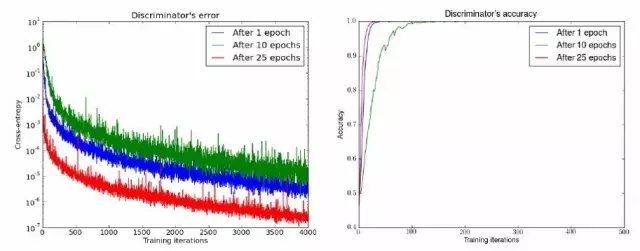
\includegraphics[width=14cm]{images/DCGAN_grandient0.jpg}
                \caption{DCGAN训练图}
                \label{fig:DCGAN梯度趋于0示意图}
                \end{figure}
            % \textcolor[rgb]{1 0 0}{todo:图片:DCGAN梯度趋于0示意图}\\
            而这会导致什么问题呢?在实践中人们发现,当D训练得更精确,G的更新会变得越差,训练变得异常地不稳定。为什么会产生这些这样的问题?为了探究背后的原因,我们就看看极端情况:判别器最优时,生成器的损失函数变成什么。给式(\ref{GAN生成器原始目标1})加上一个不依赖于生成器的项,使之变成
            \begin{align*}
            \mathbb{E}_{x\sim P_r}[\log D(x)] + \mathbb{E}_{x\sim P_g}[\log (1-D(x))]
            \end{align*}
            注意,最小化这个损失函数等价于最小化式(\ref{GAN生成器原始目标1}),而且它刚好是判别器损失函数的反。将最优判别器(\ref{最优判别器})代入上式,再进行简单的变换可以得到
            \begin{align}
            \label{公式5}
            \mathbb{E}_{x\sim P_r}\log \frac{p_r(x)}{\frac{1}{2}[p_r(x) + p_g(x)]} + E_{x\sim P_g}\log \frac{p_g(x)}{\frac{1}{2}[p_r(x)+p_g(x)]} - 2\log 2
            \end{align}
            变换成这个样子是为了引入 Kullback–Leibler divergence(简称KL散度)和 Jensen-Shannon divergence(简称JS散度)这两个重要的相似度衡量指标。
            KL散度(KL距离,前面多次介绍过)
            \begin{align*}
            KL(P_r||P_g) = \mathbb{E}_{x\sim P_r}\log \frac{p_r}{p_g}
            \end{align*}
            JS散度为
            \begin{align}
            \label{JS散度}
            JSD(P_r||P_g) = \frac{1}{2}KL \left( P_r \Big|\Big| \frac{P_r+P_g}{2} \right) + \frac{1}{2} KL\left( P_g \Big|\Big| \frac{P_r+P_g}{2} \right)
            \end{align}
            于是式(\ref{公式5})就可以继续写为
            \begin{align*}
            2JSD(P_r||P_g) - 2\log 2
            \end{align*}
            \par
            根据原始GAN定义的判别器loss,我们可以得到最优判别器的形式;而在最优判别器的下,我们可以把原始GAN定义的生成器loss等价变换为最小化真实分布$P_r$与生成分布$P_g$之间的JS散度。我们越训练判别器,它就越接近最优,最小化生成器的loss也就会越近似于最小化$P_r$和$P_g$之间的JS散度。
            \par
            梯度消失的问题就出在这个JS散度上。我们希望$P_g$与$P_r$的JS散度尽可能小,这个希望在两个分布有所重叠的时候还可以求解,但是如果两个分布完全没有重叠的部分,或者它们重叠的部分可忽略(下面解释什么叫可忽略),它们的JS散度是多少呢?答案是log2,因为对于任意一个$x$只有四种可能:
            \begin{align*}
            p_r(x) = 0 \ \text{且} \ p_g(x) = 0\\
            p_r(x) \neq 0 \ \text{且} \ p_g(x) \neq 0\\
            p_r(x) = 0 \ \text{且} \ p_g(x) \neq 0\\
            p_r(x) \neq 0 \ \text{且} \ p_g(x) = 0
            \end{align*}
            \par
            上面的第一种对计算JS散度无贡献;第二种情况由于重叠部分可忽略,所以贡献也为0;第三种情况对式(\ref{JS散度})右边第一个项的贡献是
            \begin{align*}
            \log \frac{p_g}{\frac{1}{2}(p_g+0)} = \log 2
            \end{align*}
            第4种情况与之类似,所以最终有
            \begin{align*}
            JSD(P_r||P_g) = \log 2
            \end{align*}
            换句话说,无论$ P_r $跟$ P_g $是远在天边,还是近在眼前,只要它们俩没有一点重叠或者重叠部分可忽略,JS散度就固定是常数$\log 2$,而这对于梯度下降方法意味着—梯度为0!此时对于最优判别器来说,生成器肯定是得不到一丁点梯度信息的,即使对于接近最优的判别器来说,生成器也有很大机会面临梯度消失的问题。
            \par
            但是$ P_r $与$ P_g $不重叠或重叠部分可忽略的可能性有多大?不严谨的答案是:非常大。比较严谨的答案是:当$ P_r $与$ P_g $的支撑集(support)是高维空间中的低维流形(manifold)时,$P_r $与$ P_g $重叠部分测度(measure)为0的概率为1。
            \par
            虽然论文给出的是严格的数学表述,但是直观上其实很容易理解。首先简单介绍一下这几个概念:
            \begin{enumerate}
            \item 支撑集(support)其实就是函数的非零部分子集,比如ReLU函数的支撑集就是$(0,+\infty)$,一个概率分布的支撑集就是所有概率密度非零部分的集合。
            \item 流形(manifold)是高维空间中曲线、曲面概念的拓广,我们可以在低维上直观理解这个概念,比如我们说三维空间中的一个曲面是一个二维流形,因为它的本质维度(intrinsic dimension)只有2,一个点在这个二维流形上移动只有两个方向的自由度。同理,三维空间或者二维空间中的一条曲线都是一个一维流形。
            \item 测度(measure)是高维空间中长度、面积、体积概念的拓广,可以理解为“超体积”。
            \end{enumerate}
            \par
            回过头来看第一句话,“当$ P_r $与$ P_g $的支撑集是高维空间中的低维流形时”,这基本上是成立的。因为GAN中的生成器一般是从某个低维(比如100维)的随机分布中采样出一个编码向量,再经过一个神经网络生成出一个高维样本(比如$64\times 64$的图片就有4096维)。当生成器的参数固定时,生成样本的概率分布虽然是定义在4096维的空间上,但它本身所有可能产生的变化已经被那个100维的随机分布限定了,其本质维度就是100,再考虑到神经网络带来的映射降维,最终可能比100还小,所以生成样本分布的支撑集就在4096维空间中构成一个最多100维的低维流形,“撑不满”整个高维空间。
            \par
            “撑不满”就会导致真实分布与生成分布难以“碰到面”,这很容易在二维空间中理解:一方面,二维平面中随机取两条曲线,它们之间刚好存在重叠线段的概率为0;另一方面,虽然它们很大可能会存在交叉点,但是相比于两条曲线而言,交叉点比曲线低一个维度,长度(测度)为0,可忽略。三维空间中也是类似的,随机取两个曲面,它们之间最多就是比较有可能存在交叉线,但是交叉线比曲面低一个维度,面积(测度)是0,可忽略。从低维空间拓展到高维空间,就有了如下逻辑:因为一开始生成器随机初始化,所以$ P_g $几乎不可能与$P_r$有什么关联,所以它们的支撑集之间的重叠部分要么不存在,要么就比$ P_r $和$ P_g $的最小维度还要低至少一个维度,故而测度为0。所谓“重叠部分测度为0”,就是上文所言“不重叠或者重叠部分可忽略”的意思。
            \par
            至此,就得到了文献\cite{2017.Arjovsky}中关于生成器梯度消失的第一个论证:在(近似)最优判别器下,最小化生成器的loss等价于最小化$ P_r $与$ P_g $之间的JS散度,而由于$ P_r $与$ P_g $几乎不可能有不可忽略的重叠,所以无论它们相距多远JS散度都是常数$\log 2$,最终导致生成器的梯度(近似)为0,梯度消失。
            \par
            接着作者从第二个角度进行论证,但是背后的思想也可以直观地解释:首先,$P_r $与$ P_g $之间几乎不可能有不可忽略的重叠,所以无论它们之间的“缝隙”多狭小,都肯定存在一个最优分割曲面把它们隔开,最多就是在那些可忽略的重叠处隔不开而已。
            由于判别器作为一个神经网络可以无限拟合这个分隔曲面,所以存在一个最优判别器,对几乎所有真实样本给出概率1,对几乎所有生成样本给出概率0,而那些隔不开的部分就是难以被最优判别器分类的样本,但是它们的测度为0,可忽略。
            最优判别器在真实分布和生成分布的支撑集上给出的概率都是常数(1和0),导致生成器的loss梯度为0,梯度消失。
            \par
            有了上述的理论分析,原始GAN不稳定的原因就彻底清楚了:判别器训练得太好,生成器梯度消失,生成器loss降不下去;判别器训练得不好,生成器梯度不准,四处乱跑。只有判别器训练得不好不坏才行,但是这个火候又很难把握,甚至在同一轮训练的前后不同阶段这个火候都可能不一样,所以GAN才那么难训练。实验辅证如下图(\ref{fig:生成器梯度轨迹})所示
                \begin{figure}[H]
                \centering
                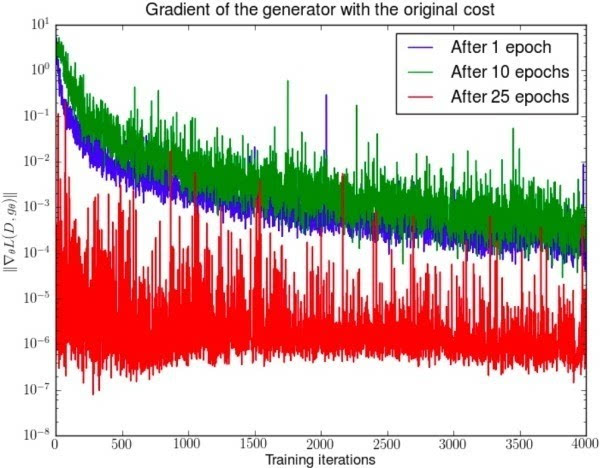
\includegraphics[width=8cm]{images/Generator_gradient_trajectory.jpg}
                \caption{生成器梯度轨迹}
                \label{fig:生成器梯度轨迹}
                \end{figure}
            % \textcolor[rgb]{1 0 0}{todo:图片:生成器梯度轨迹}\\
            先分别将DCGAN训练1、20、25个epoch,然后固定生成器不动,判别器重新随机初始化从头开始训练,对于第一种形式的生成器loss产生的梯度可以打印出其尺度的变化曲线,可以看到随着判别器的训练,生成器的梯度均迅速衰减。注意$y$轴是对数坐标轴。
            \par
            上面只是在直观上分析了GAN存在的问题,下面给出文献\cite{2017.Arjovsky}的理论分析:
            \begin{lemma}[Lemma1 ]
            设$g:\mathcal{Z}\to \mathcal{X}$是一个由仿射变换和逐点定义的非线性函数(ReLU、leaky ReLU或者诸如sigmoid、tanh、softplus之类的光滑严格递增函数)复合得到的复合函数,则$g(\mathcal{Z})$包含在可数多个流形的并集中,并且它的维数至多为$\dim(\mathcal{Z})$。因此,若$\dim(\mathcal{Z}) < \dim(\mathcal{X})$,则$g(\mathcal{Z})$在X中测度为0。
            \end{lemma}
            \par
            Lemma1表明,若generator(G)是一个神经网络,并且G的输入(随机高斯噪声)的维数比产生的图像的维数低,则无论怎样训练,G也只能产生整个图像空间中很小的部分,有多小呢?它在图像空间中只是一个零测集。
            \par
            训练GAN时,训练集总归是有限的,$P_r$一般可以看成是低维的流形;如果$P_g$也是低维流形,或者它与$P_r$的支撑集没有交集,则在 (D)达到最优时,JSD就会被最大化。D达到最优将导致G的梯度变得异常地差,训练将变得异常不稳定。
            下面的几个定理、引理就是证明$P_g$在上述两种情况下,最优的D是存在的。
            \begin{theorem}[Theorem2.1]
            若分布$P_r$和$P_g$的支撑集分别包含在两个无交紧致子集$\mathcal{M}$和$\mathcal{P}$中,则存在一个光滑的最优 $D*: \mathcal{X} \to [0,1]$,它的精度是1,并且,对任意的
            $x\in \mathcal{M} \cup \mathcal{P}$有
            \begin{align*}
            \nabla _x D^*(x) = 0
            \end{align*}
            \end{theorem}
            \par
            定理2.1表示:如果两个概率分布的支撑集没有交集,则完美的D总是存在的,并且(在两个分布的支撑集的并集上)D的梯度为0,也就是说,这时候任何梯度算法都将失效。这就是GAN训练的时候,(在两个概率分布的支撑集没有交集的情况下)当D训练效果很好的时候,G的更新将变得很差的原因。
            \begin{lemma}[Lemma 2]
            设$\mathcal{M}$和$\mathcal{P}$是$R^d$的两个非满维度的正则子流形,再设$\eta$和$\eta'$ 是任意的两个独立连续随机变量,定义两个扰动流形$\tilde{\mathcal{M}} = \mathcal{M} + \eta$,$\tilde{\mathcal{P}}= \mathcal{P} + \eta'$,则
            \begin{align*}
            P_{\eta,\eta'}(\tilde{\mathcal{M}}\text{不与}\tilde{\mathcal{P}}\text{完美对齐}) = 1
            \end{align*}
            \end{lemma}
            \par
            Lemma 2是为定理2.2做准备,它表明任意两个非满维的正则子流形都可以通过微小的扰动使得它们不是完美对齐(notperfectly align)的,即它们的交点都是横截相交(intersect transversally)的。在这里形象地说明一下横截相交和完美对齐:
            横截相交(intersect transversally):对两个子流形,在任意一个交点处,两者的切平面能够生成整个空间,则称两个子流形横截相交。当然,如果它们没有交集,则根据定义,它们天然就是横截相交的。下图(\ref{fig:横截相交示意图})给出了一个示例
                \begin{figure}[H]
                \centering
                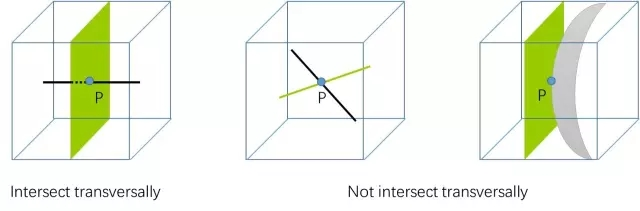
\includegraphics[width=8cm]{images/Cross_intersecting.jpg}
                \caption{横截相交示意图}
                \label{fig:横截相交示意图}
                \end{figure}
            % \textcolor[rgb]{1 0 0}{todo:图片:横截相交示意图}\\
            在交点P处,平面的切平面是其自身,直线的切平面也是其自身,它们可以张成全空间,因此是横截相交的,而两个直线没办法张成全空间,因此不是横截相交的;如果两个流形是相切的,在切点处它们的切平面是相同的,也不可能张成全空间,因此也不是横截相交的。
            完美对齐(perfectly align): 如果两个子流形有交集,并且在某个交点处,它们不是横截相交的。
            \par
            $P_r$和$P_g$的支撑集如果存在交集,那么根据Lemma2,我们总可以通过微小的扰动使得它们不是完美对齐的,也就是说,它们是横截相交的。
            \begin{lemma}[Lemma 3]
            设$\mathcal{M}$和$\mathcal{P}$是$R^d$的两个非完美对齐,非满维的正则子流形,$\mathcal{L} = \mathcal{M}\cap \mathcal{P} $,若$\mathcal{M}$和$\mathcal{P}$无界,则$\mathcal{L}$也是一个流形,且维数严格低于$\mathcal{M}$和$\mathcal{P}$的维数。若它们有界,则$\mathcal{L}$是至多四个维数严格低于全空间的流形之并。无论哪种情形,$\mathcal{L}$在$\mathcal{M}$或者$\mathcal{P}$中的测度均为0。
            \end{lemma}
            \par
            Lemma 3说的是,两个正则子流形(满足一定条件:非完美对齐,非满维)的交集的维数要严格低于它们自身的维数。也就是说,它们的交集只是冰山一角,小到相对它们自身可以忽略。对于$P_r$和$P_g$的支撑集来说,根据Lemma 2,我们总可以通过微小扰动使得它们是非完美对齐的,在根据Lemma 3,$P_r$和$P_g$的交集是微不足道。
            \begin{theorem}[Theorem2.2]
            设$P_r$和$P_g$分别是支撑集包含在闭流形$\mathcal{M}$和$\mathcal{P}$中的两个分布,且它们非完美对齐、非满维。进一步地,我们假设$P_r$和$P_g$在各自的流形中分别连续,即:若集合A在$\mathcal{M}$中测度为0,则$P_r(A) = 0$(在$P_g$上也有类似结果),则存在精度为1的最优$ D^*:\mathcal{X}\to [0,1]$,并且几乎对$\mathcal{M}$或者$\mathcal{P}$中的任意点$x$,$D^*$在$x$的任意邻域内总是光滑的,且有
            \begin{align*}
            \nabla_x D^*(x) = 0
            \end{align*}
            \end{theorem}
            \par
            定理2.1证明的是对于$P_r$和$P_g$无交的情形下,最优的D是存在的。定理2.2承接Lemma 3,证明了在$P_r$和$P_g$的支撑集有交集,且横截相交的情况下,最优的D是存在的。这两个定理实际上把两种可能导致D最优,且梯度消失的情形在理论上做出证明,由于梯度的消失,G的更新将得不到足够的梯度,导致G很差。
            \begin{theorem}[Theorem2.3]
            在定理2.2的条件下,有
            \begin{align*}
            & JSD(P_r||P_g) = \log 2\\
            & KL(P_r||P_g) = +\infty\\
            & KL(P_g||P_r) = +\infty
            \end{align*}
            \end{theorem}
            \par
            定理2.3表明,随着D越来越好,D的loss将越来越小,趋于0,因此$P_r$和$P_g$的JSD被最大化,达到最大值$\log2$,这时,$P_r$和$P_g$的交叉熵达到无穷大,也就是说,即使两个分布之间的差异任意地小,它们之间的KL散度仍然会被最大化,趋于无穷。这是什么意思呢?利用KL散度来衡量分布间的相似性在这里并不是一个好的选择。因此,我们有必要寻求一个更好的衡量指标。
            \begin{theorem}[Theorem2.4 (Vanishing gradients on the generator)]
            设$g_\theta:\mathcal{Z}\to \mathcal{X}$是一个可微函数,有它导出分布$P_g$。再设$P_r$为真实数据分布,$D$是一个可微的discriminator。如果 Theorem 2.1 和 Theorem 2.2 的条件能够满足,且$\forall \varepsilon>0 $,$||D-D^*||<\varepsilon$,以及$\exists M>0$,$\mathbb{E}_{z\sim p(z)}\left[||J_\theta g_\theta(z)||_2^2\right] \leqslant M^2$,则
            \begin{align*}
            ||\nabla_\theta \mathbb{E}_{z\sim p(z)}\left[\log(1-D(g_\theta(z)))\right]||_2 <M\frac{\epsilon}{1-\epsilon}
            \end{align*}
            \end{theorem}
            \begin{Proof}
            在证明Theorem2.1和Theorem2.2时,我们说$D^*$在$P_g$的支撑集上是locally 0。基于此,我们对 the support使用Jensen不等式和chain rule,有
            \begin{align*}
            ||\nabla_\theta \mathbb{E}_{z\sim p(z)}\left[\log(1-D(g_\theta(z)))\right]||_2^2 &\leqslant \mathbb{E}_{z\sim p(z)}\left[ \frac{||\nabla_\theta D(g_\theta(z))||_2^2}{|1-D(g_\theta(z))|^2} \right]\\
            & \leqslant \mathbb{E}_{z\sim p(z)}\left[ \frac{||\nabla_\theta D(g_\theta(z))||_2^2||J_\theta g_\theta(z)||_2^2}{|1-D(g_\theta(z))|^2} \right]\\
            &<\mathbb{E}_{z\sim p(z)}\left[ \frac{(||\nabla_\theta D(g_\theta(z))||_2+\epsilon)^2||J_\theta g_\theta(z)||_2^2}{(|1-D(g_\theta(z))|-\epsilon)^2} \right]\\
            &=\mathbb{E}_{z\sim p(z)} \left[\frac{\epsilon^2||J_{\theta}g_\theta(z)||_2^2}{(1-\epsilon)^2}  \right]\\
            & \leqslant M^2\frac{\epsilon^2}{(1-\epsilon)^2}
            \end{align*}
            由此得到
            \begin{align*}
            ||\nabla_\theta \mathbb{E}_{z\sim p(z)}\left[\log(1-D(g_\theta(z)))\right]||_2 <M\frac{\epsilon}{1-\epsilon}
            \end{align*}
            $\square$
            \end{Proof}
            \par
            定理2.4 探究了generator在前面所述情况下回出现什么问题,它说明了若G采用original cost function(零和博弈),那么它的梯度的上界被D与最优的$D^*$之间的距离bound住。通俗的说,我们训练GAN的时候,D越接近最优的$D^*$,则G的梯度就越小,如果梯度太小了,梯度算法不能引导G变得更好。
            \begin{corollary}[corollary 2.1]
            在定理2.4的假设下,有
            \begin{align*}
            \lim_{||D-D^*||\to 0}\nabla_\theta \mathbb{E}_{z\sim p(z)}[\log (1-D(g_\theta(z)))]=0
            \end{align*}
            \end{corollary}
            推论2.1是定理2.4的极限情况。
        \subsubsection{第二种原始GAN形式的问题}
            \par
            第二种原始GAN形式(\ref{GAN生成器原始目标2})的问题是:最小化第二种生成器loss函数,会等价于最小化一个不合理的距离衡量,这导致两个问题,一是梯度不稳定,二是collapse mode即多样性不足。文献\cite{2017.Arjovsky}又是从两个角度进行了论证:
            \par
            如前文所说,Ian Goodfellow提出的“- log D trick”是把生成器loss改成
            \begin{align}
            \label{公式3}
            \mathbb{E}_{x\sim P_g}[-\log D(x)]
            \end{align}
            上文推导已经得到在最优判别器$D^*$下
            \begin{align}
            \label{公式9}
            \mathbb{E}_{x\sim P_r}[\log D^*(x)] + \mathbb{E}_{x\sim P_g}[\log(1-D^*(x))] = 2JSD(P_r || P_g) - 2\log 2
            \end{align}
            可以把KL散度(注意下面是先$g$后$r$)变换成含$D^*$的形式:
            \begin{align}
            \label{公式10}
            KL(P_g || P_r) &= \mathbb{E}_{x \sim P_g} [\log \frac{p_g(x)}{p_r(x)}] \notag\\
            &= \mathbb{E}_{x \sim P_g} \left[\log \frac{p_g(x) / (p_r(x) + p_g(x))}{p_r(x) / (p_r(x) + p_g(x))}\right] \notag\\
            &= \mathbb{E}_{x \sim P_g} \left[\log \frac{1 - D^*(x)}{D^*(x)}\right] \notag\\
            &= \mathbb{E}_{x \sim P_g} \log [1 - D^*(x)] - \mathbb{E}_{x \sim P_g} \log D^*(x)
            \end{align}
            由式(\ref{公式9})(\ref{公式10})可得最小化目标的等价变形
            \begin{align}
            \mathbb{E}_{x \sim P_g} [-\log D^*(x)] &= KL(P_g || P_r) - \mathbb{E}_{x \sim P_g} \log [1 - D^*(x)] \notag \\ &= KL(P_g || P_r) - 2JSD(P_r || P_g) + 2\log 2 + \mathbb{E}_{x\sim P_r}[\log D^*(x)]
            \end{align}
            注意上式最后两项不依赖于生成器G,最终得到最小化(\ref{公式3})等价于最小化
            \begin{align}
            \label{公式11}
            KL(P_g || P_r) - 2JSD(P_r || P_g)
            \end{align}
            \par
            这个等价最小化目标存在两个严重的问题。第一是它同时要最小化生成分布与真实分布的KL散度,却又要最大化两者的JS散度,一个要拉近,一个却要推远!这在直观上非常荒谬,在数值上则会导致梯度不稳定,这是后面那个JS散度项的问题。
            \par
            第二,即便是前面那个正常的KL散度项也有毛病。因为KL散度不是一个对称的衡量,$KL(P_g || P_r)$与$KL(P_r || P_g)$是有差别的。以前者为例
            \begin{enumerate}
                \item 当$P_g(x)\rightarrow 0$而$P_r(x)\rightarrow 1$时,$P_g(x) \log \frac{P_g(x)}{P_r(x)} \rightarrow 0$,对$KL(P_g || P_r)$贡献趋近0;
                \item 当$P_g(x)\rightarrow 1$而$P_r(x)\rightarrow 0$时,$P_g(x) \log \frac{P_g(x)}{P_r(x)} \rightarrow +\infty$,对$KL(P_g || P_r)$贡献趋近正无穷。
            \end{enumerate}
            \par
            换言之,$KL(P_g || P_r)$对于上面两种错误的惩罚是不一样的,第一种错误对应的是“生成器没能生成真实的样本”,惩罚微小;第二种错误对应的是“生成器生成了不真实的样本” ,惩罚巨大。第一种错误对应的是缺乏多样性,第二种错误对应的是缺乏准确性。这一放一打之下,生成器宁可多生成一些重复但是很“安全”的样本,也不愿意去生成多样性的样本,因为那样一不小心就会产生第二种错误,得不偿失。这种现象就是大家常说的collapse mode。下面,我们给出文献\cite{2017.Arjovsky}中的理论分析:
            \begin{theorem}[Theorem 2.5]
            设连续分布$P_r$和$P_{g_\theta}$的密度函数为$p_r$和$p_{g_\theta}$。在参数为$\theta=\theta_0$时的最优生成器为
            \begin{align*}
            D^*=\frac{p_r}{p_{g_{\theta_0}}+p_r}
            \end{align*}
            则
            \begin{align*}
            \mathbb{E}_{z\sim p(z)}[-\nabla _\theta\log D^*(g_\theta(z))|_{\theta=\theta_0}] = \nabla_\theta[KL(P_{g_\theta}||P_r) - 2JSD(P_{g_\theta}||P_r)]|_{\theta=\theta_0}
            \end{align*}
            \end{theorem}
            \begin{Proof}
            从GAN的原始论文我们已经知道
            \begin{align*}
            \mathbb{E}_{z\sim p(z)}[\nabla_\theta \log(1-D^*(g_\theta(z)))|_{\theta=\theta_0}] = \nabla_\theta 2JSD(P_{g_\theta}||P_r)|_{\theta=\theta_0}
            \end{align*}
            此外,Huszar于2016指出
            \begin{align*}
            KL(P_{g_\theta}||P_r) & = \mathbb{E}_{x\sim P_{g_\theta}}\left[ \log\frac{p_{g_\theta(x)}}{p_r(x)} \right]\\
            & =\mathbb{E}_{x\sim P_{g_\theta}}\left[ \log\frac{p_{g_{\theta_0}(x)}}{p_r(x)} \right] - \mathbb{E}_{x\sim P_{g_\theta}}\left[ \frac{p_{g_\theta}(x)}{p_{g_{\theta_0}}(x)} \right]\\
            &=-\mathbb{E}_{x\sim P_{g_\theta}}\left[ \log \frac{D^*(x)}{1-D^*(x)} \right]-KL(P_{g_\theta}||P_{g_{\theta_0}})\\
            &=-\mathbb{E}_{z\sim p(z)}\left[ \log \frac{D^*(g_\theta(z))}{1-D^*(g_\theta(z))} \right]-KL(P_{g_\theta}||P_{g_{\theta_0}})
            \end{align*}
            在$\theta = \theta_0$处求导,我们有
            \begin{align*}
            \nabla_\theta KL(P_{g_\theta}||P_{g_{\theta_0}}) &= -\nabla_\theta\mathbb{E}_{z\sim p(z)} \left[\log \frac{D^*(g_\theta(z))}{1-D^*(g_\theta(z))}\right]\Big|_{\theta=\theta_0} - \nabla_\theta KL(P_{g_\theta}||P_{g_{\theta_0}})|_{\theta=\theta_0}\\
            &=\mathbb{E}_{z\sim p(z)} \left[-\nabla_\theta\log \frac{D^*(g_\theta(z))}{1-D^*(g_\theta(z))}\right]\Big|_{\theta=\theta_0}
            \end{align*}
            用JSD减去上述等式,即可得到Theorem 2.5。$\square$
            \end{Proof}
            \par
            定理2.5研究了G的loss为the$ -\log D$ cost时将会出现的问题。我们可以看到,JSD越大G的梯度反而会越小,也就是说,它可能会引导两个分布往相异的方向,此外,上式的KL项虽对产生无意义图像会有很大的惩罚,但是对mode collapse惩罚很小,也就是说,GAN训练时很容易落入局部最优,产生mode collapse。KL散度不是对称的,但JSD是对称的,因此JSD并不能改变这种状况。这就是我们在训练GAN时经常出现mode collapse的原因。
            \begin{theorem}[Theorem 2.6 Instability of generator gradient updates]
            设$g_\theta:\mathcal{Z}\to \mathcal{X}$是一个可微函数,由它可导出分布$P_g$。再设$P_r$为真实数据的分布,且满足定理2.1或者定理2.2的条件之一。令$D$是一个discriminator,满足$D^* - D = \epsilon$为高斯白噪声,且$\nabla_x D^* - \nabla_x D = r$也为高斯白噪声,则有
            \begin{align*}
            \mathbb{E}_{z\sim p(z)} [-\nabla_\theta \log D(g_\theta(z))]
            \end{align*}
            的每一维均服从期望和方差为正无穷的中心化柯西分布。
            \end{theorem}
            \par
            定理2.6告诉我们,若G采用the –$\log D$ cost,在定理2.1或者定理2.2的条件下,当$D$与$D^*$足够接近时,G的梯度会呈现强烈震荡,这也就是说,G的更新会变得很差,可能导致GAN训练不稳定。
            \par
            实验辅证如下图(\ref{fig:WGAN前作Figure 3})所示
                \begin{figure}[H]
                \centering
                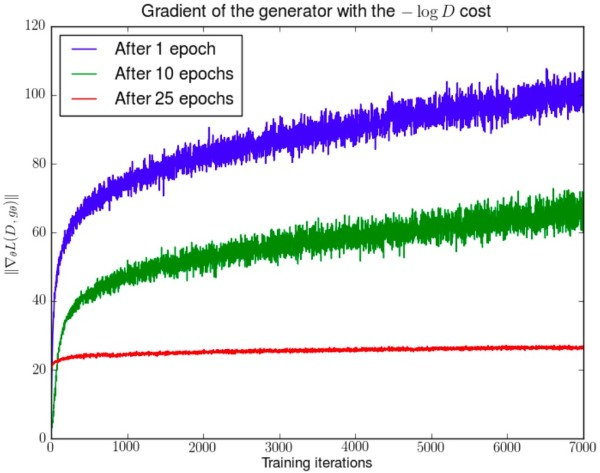
\includegraphics[width=8cm]{images/WGAN_make_Figure3.jpg}
                \caption{DCGAN训练1、20、25个epoch的训练结果}
                \label{fig:WGAN前作Figure 3}
                \end{figure}
            % \textcolor[rgb]{1 0 0}{todo:图片:WGAN前作Figure 3}\\
            先分别将DCGAN训练1、20、25个epoch,然后固定生成器不动,判别器重新随机初始化从头开始训练,对于第二种形式的生成器loss产生的梯度可以打印出其尺度的变化曲线,可以看到随着判别器的训练,蓝色和绿色曲线中生成器的梯度迅速增长,说明梯度不稳定,红线对应的是DCGAN相对收敛的状态,梯度才比较稳定。
            \par
            图(\ref{fig:WGAN前作Figure 3})给出了定理2.6的实验模拟的效果,在DCGAN尚未收敛时,固定G,训练D将导致G的梯度产生强烈震荡。当DCGAN收敛时,这种震荡得到有效的抑制。
        \subsubsection{WGAN之前的一个过渡解决方案}
            \par
            原始GAN问题的根源可以归结为两点,一是等价优化的距离衡量(KL散度、JS散度)不合理,二是生成器随机初始化后的生成分布很难与真实分布有不可忽略的重叠。
            \par
            文献\cite{2017.Arjovsky}针对第二点提出了一个解决方案,就是对生成样本和真实样本加噪声。直观上说,使得原本的两个低维流形“弥散”到整个高维空间,强行让它们产生不可忽略的重叠。而一旦存在重叠,JS散度就能真正发挥作用,此时如果两个分布越靠近,它们“弥散”出来的部分重叠得越多,JS散度也会越小而不会一直是一个常数,于是(在第一种原始GAN形式下)梯度消失的问题就解决了。在训练过程中,我们可以对所加的噪声进行退火(annealing),慢慢减小其方差,到后面两个低维流形“本体”都已经有重叠时,就算把噪声完全拿掉,JS散度也能照样发挥作用,继续产生有意义的梯度把两个低维流形拉近,直到它们接近完全重合。以上就是对原文的直观解释。
            \par
            既然general GAN采用的loss不是一种好的选择,有什么loss能够有效避免这种情形吗?
            一个可行的方案是\uline{打破定理的条件,给D的输入添加噪声}。后续的几个定理对添加噪声的方法作了回答。
            \par
            在这个解决方案下我们可以放心地把判别器训练到接近最优,不必担心梯度消失的问题。而当判别器最优时,可得判别器的最小loss为
            \begin{align}
            \min L_D(P_{r+\epsilon}, P_{g+\epsilon}) &= - \mathbb{E}_{x\sim P_{r+\epsilon}}[\log D^*(x)] - \mathbb{E}_{x\sim P_{g+\epsilon}}[\log(1-D^*(x))] \\ &= 2\log 2 - 2JSD(P_{r+\epsilon} || P_{g+\epsilon})
            \end{align}
            其中$P_{r+\epsilon}$和$P_{g+\epsilon}$分别是加噪后的真实分布与生成分布。反过来说,从最优判别器的loss可以反推出当前两个加噪分布的JS散度。两个加噪分布的JS散度可以在某种程度上代表两个原本分布的距离,也就是说可以通过最优判别器的loss反映训练进程!不过,因为加噪JS散度的具体数值受到噪声的方差影响,随着噪声的退火,前后的数值就没法比较了,所以它不能成为$P_r$和$P_g$距离的本质性衡量。
            \begin{theorem}[Theorem 3.1]
            若$X$满足分布$P_X$,且它的支撑集落在$\mathcal{M}$中,$\epsilon$是一个密度函数为$p_\epsilon$的绝对连续分布,则$P_{X+\epsilon}$也是一个绝对连续分布,具有密度函数
            \begin{align*}
            p_{X+\epsilon} = \mathbb{E}_{y\sim P_X}[p_\epsilon(x-y)]\\
            =\int_\mathcal{M}p_{\epsilon}(x-y)\mathrm{d}P_X(y)
            \end{align*}
            \end{theorem}
            \begin{corollary}[corollary 3.1]
            \begin{enumerate}
            \item 如果$\epsilon \sim N(0,\sigma^2I)$,则
            \begin{align*}
            p_{X+\epsilon}(x) = \frac{1}{Z}\int_\mathcal{M}e^{-\frac{||y-x||^2}{2\sigma^2}}\mathrm{d}P_X(y)
            \end{align*}
            \item 如果$\epsilon\sim N(0,\Sigma)$,则
            \begin{align*}
            p_{X+\epsilon}(x) = \frac{1}{Z}\mathbb{E}_{y\sim P_X}\left[e^{-\frac{1}{2}||y-x||_{\Sigma^{-1}}^2}\right]
            \end{align*}
            \item 如果$p_\epsilon(x)\propto \frac{1}{||x||^{d+1}}$,则
            \begin{align*}
            p_{X+\epsilon}(x) = \frac{1}{Z}\mathbb{E}_{y\sim P_X}\left[\frac{1}{||x-y||^{d+1}}\right]
            \end{align*}
            \end{enumerate}
            \end{corollary}
            \par
            定理3.1和推论3.1表明,$\epsilon$的分布会影响我们对距离的选择。对于$P_{g+\epsilon}$和$P_{r+\epsilon}$,此时的最优判别器为
            \begin{align*}
            D^*(x) = \frac{p_{r_\epsilon(x)}}{p_{r+\epsilon}(x)+p_{g+\epsilon}(x)}
            \end{align*}

            \begin{theorem}[Theorem 3.2]
            设$P_r$和$P_g$分别是支撑集落在$\mathcal{M}$和$\mathcal{P}$中的两个分布,且$\epsilon \sim N(0,\sigma^2I)$,则梯度具有以下形式
            \begin{align*}
            \mathbb{E}_{z\sim p(z)}[\nabla_\theta \log (1-D^*(g_\theta(z)))] &= \mathbb{E}_{z\sim p(z)}\bigg[ a(z)\int_\mathcal{M}p_\epsilon(g_\theta(z)-y)\nabla_\theta||g_\theta(z)-y||^2\mathrm{d}P_r(y)\\
            &\quad -b(z)\int_\mathcal{P}p_\epsilon(g_\theta(z)-y)\nabla_\theta||g_\theta(z)-y||^2\mathrm{d}P_g(y)\bigg]
            \end{align*}
            其中:$a(z),b(z)$是两个正值函数。更进一步的,$b>a$当且仅当$p_{r+\epsilon} > p_{g+\epsilon}$;$b<a$当且仅当$p_{r+\epsilon} < p_{g+\epsilon}$。
            \end{theorem}
            \par
            定理3.2证明了G的梯度可以分为两项,第一项表明,G会被引导向真实数据分布移动,第二项表明,G会被引导向概率很高的生成样本远离。作者指出,上述的梯度格式具有一个很严重的问题,那就是由于$g(\mathcal{Z})$是零测集,D在优化时将忽略该集合;然而G却只在该集合上进行优化。进一步地,这将导致D极度容易受到生成样本的影响,产生没有意义的样本。
            \begin{corollary}[corollary 3.2]
            设$\epsilon,\epsilon'\sim N(0,\sigma^2I)$以及$\tilde{g}_{\theta}(z)=g_\theta(z)+\epsilon' $,则
            \begin{align*}
            \mathbb{E}_{z\sim p(z),\epsilon'}[\nabla_\theta\log (1-D^*(\tilde{g}_\theta(z)))]& = \mathbb{E}_{z\sim p(z),\epsilon'} \bigg[a(z)\int_\mathcal{M}p_\epsilon(\tilde{g}_\theta(z)-y)\nabla_\theta||\tilde{g}_\theta(z)-y||^2 \mathrm{d}P_r(y) \\
            &\quad -b(z)\int_\mathcal{P}p_\epsilon(\tilde{g}_\theta(z)-y)\nabla_\theta||\tilde{g}_\theta(z)-y||^2\mathrm{d}P_g(y)\bigg]\\
            &=2\nabla_\theta JSD(P_{r+\epsilon}||P_{g+\epsilon})
            \end{align*}
            \end{corollary}
            \par
            上述推论中的$a,b$和Theorem3.2相同,主要的不同是对D的输入添加噪声,在训练的过程中将引导噪声样本向真实数据流形的方向移动,这可以看成是引导样本的一个小邻域向真实数据移动。这可以解决D极度容易受到生成样本的影响的问题。
            \begin{Proof}
            在求解生成器时,判别器是固定的,$g_\theta(z)$是唯一依赖于$\theta$的量(for every $z$)。对我们的损失函数求导,有
            \begin{align*}
            &\mathbb{E}_{z\sim p(z)}[\nabla_\theta\log(1-D^*(g_\theta(z)))]\\
            ={}&\mathbb{E}_{z\sim p(z)}\left[ \nabla_\theta\log \frac{p_{g+\epsilon}(g_\theta(z))}{p_{r+\epsilon}(g_\theta(z))+ p_{g+\epsilon}(g_\theta(z))}   \right]\\
            ={}&\mathbb{E}_{z\sim p(z)}\left[ \nabla_\theta\log p_{g+\epsilon}(g_\theta(z))- \nabla_\theta\log (p_{r+\epsilon}(g_\theta(z))+p_{g+\epsilon}(g_\theta(z)))  \right]\\
            ={}&\mathbb{E}_{z\sim p(z)}\left[ \frac{\nabla_\theta p_{g+\epsilon}(g_\theta(z))}{p_{g+\epsilon}(g_\theta(z))} - \frac{\nabla_\theta p_{g+\epsilon}(g_\theta(z))+\nabla_\theta p_{r+\epsilon}(g_\theta(z))}{p_{g+\epsilon}(g_\theta(z))+ p_{r+\epsilon}(g_\theta(z))}    \right]\\
            ={}&\mathbb{E}_{z\sim p(z)}\bigg[ \frac{1}{p_{g+\epsilon}(g_\theta(z))+ p_{r+\epsilon}(g_\theta(z))} \nabla_\theta[p_{r+\epsilon}(g_\theta(z))] \\
            & \quad -  \frac{1}{p_{g+\epsilon}(g_\theta(z))+ p_{r+\epsilon}(g_\theta(z))} \frac{p_{r+\epsilon}(g_\theta(z))}{p_{g+\epsilon}(g_\theta(z))}\nabla_\theta[p_{g+\epsilon}(g_\theta(z))]
             \bigg]
            \end{align*}
            令$\epsilon$的密度为$\frac{1}{Z}e^{-\frac{||x||^2}{2\sigma^2}}$。现在,我们定义
            \begin{align*}
            & a(z) = \frac{1}{2\sigma^2} \frac{1}{p_{g+\epsilon}(g_\theta(z))+ p_{r+\epsilon}(g_\theta(z))}\\
            & b(z) = \frac{1}{2\sigma^2} \frac{1}{p_{g+\epsilon}(g_\theta(z))+ p_{r+\epsilon}(g_\theta(z))}\frac{p_{r+\epsilon}(g_\theta(z))}{p_{g+\epsilon}(g_\theta(z))}
            \end{align*}
            前面我们说$a,b$是正实数。根据$a,b$的表达式,我们有$b=a\frac{p_{r+\epsilon}}{p_{g+\epsilon}}$,并且$b>a$当且仅当$p_{r+\epsilon}>p_{g+\epsilon}$,以及$b<a$当且仅当$p_{r+\epsilon}<p_{g+\epsilon}$,这正是我们想要的。继续上面的证明,有
            \begin{align*}
            &\mathbb{E}_{z\sim p(z)}[\nabla_\theta\log(1-D^*(g_\theta(z)))]\\
            ={}&\mathbb{E}_{z\sim p(z)}[2\sigma^2a(z)\nabla_\theta[-p_{r+\epsilon}(g_\theta(z))] - 2\sigma^2b(z)\nabla_\theta[-p_{g+\epsilon}(g_\theta(z))]]\\
            ={}&\mathbb{E}_{z\sim p(z)}\biggl[ 2\sigma^2a(z)\int_\mathcal{M}-\nabla_\theta \frac{1}{Z}e^{-\frac{||g_\theta(z)-y||_2^2}{2\sigma^2}}\mathrm{d}p_r(y) \\
            &\quad -  2\sigma^2b(z)\int_\mathcal{P}-\nabla_\theta \frac{1}{Z}e^{-\frac{||g_\theta(z)-y||_2^2}{2\sigma^2}}\mathrm{d}p_g(y)  \biggr]\\
            ={}&\mathbb{E}_{z\sim p(z)}\biggl[ a(z)\int_\mathcal{M} \frac{1}{Z}e^{-\frac{||g_\theta(z)-y||_2^2}{2\sigma^2}}\nabla_\theta ||g_\theta(z)-y||^2 \mathrm{d}p_r(y) \\
            & \quad -  b(z)\int_\mathcal{P}\frac{1}{Z}e^{-\frac{||g_\theta(z)-y||_2^2}{2\sigma^2}}\nabla_\theta ||g_\theta(z)-y||^2\mathrm{d}p_g(y)  \biggr]\\
            ={}&\mathbb{E}_{z\sim p(z)}\biggl[ a(z)\int_\mathcal{M} p_\epsilon(g_\theta(z)-y) \nabla_\theta ||g_\theta(z)-y||^2 \mathrm{d}p_r(y) \\
            &\quad -  b(z)\int_\mathcal{P} p_\epsilon(g_\theta(z)-y)\nabla_\theta ||g_\theta(z)-y||^2\mathrm{d}p_g(y)  \biggr]
            \end{align*}
            % \begin{align*}
            % &\mathbb{E}_{z\sim p(z)}[\nabla_\theta\log(1-D^*(g_\theta(z)))]\\
            % ={}&\mathbb{E}_{z\sim p(z)}[2\sigma^2a(z)\nabla_\theta[-p_{r+\epsilon}(g_\theta(z))] - 2\sigma^2b(z)\nabla_\theta[-p_{g+\epsilon}(g_\theta(z))]]\\
            % ={}&\mathbb{E}_{z\sim p(z)}\left[ 2\sigma^2a(z)\int_\mathcal{M}-\nabla_\theta \frac{1}{Z}e^{-\frac{||g_\theta(z)-y||_2^2}{2\sigma^2}}\mathrm{d}p_r(y) -  2\sigma^2b(z)\int_\mathcal{P}-\nabla_\theta \frac{1}{Z}e^{-\frac{||g_\theta(z)-y||_2^2}{2\sigma^2}}\mathrm{d}p_g(y)  \right]\\
            % ={}&\mathbb{E}_{z\sim p(z)}\biggl[ a(z)\int_\mathcal{M} \frac{1}{Z}e^{-\frac{||g_\theta(z)-y||_2^2}{2\sigma^2}}\nabla_\theta ||g_\theta(z)-y||^2 \mathrm{d}p_r(y) \\
            % & \quad -  b(z)\int_\mathcal{P}\frac{1}{Z}e^{-\frac{||g_\theta(z)-y||_2^2}{2\sigma^2}}\nabla_\theta ||g_\theta(z)-y||^2\mathrm{d}p_g(y)  \biggr]\\
            % ={}&\mathbb{E}_{z\sim p(z)}\biggl[ a(z)\int_\mathcal{M} p_\epsilon(g_\theta(z)-y) \nabla_\theta ||g_\theta(z)-y||^2 \mathrm{d}p_r(y) \\
            % &\quad -  b(z)\int_\mathcal{P} p_\epsilon(g_\theta(z)-y)\nabla_\theta ||g_\theta(z)-y||^2\mathrm{d}p_g(y)  \biggr]
            % \end{align*}
            Finishing the proof. $\square$
            \end{Proof}
            \begin{definition}[Wasserstein距离]
            $\mathcal{X}$上的两个分布$P,Q$的Wasserstein距离/度量/散度$W(P,Q)$定义为
            \begin{align*}
            W(P,Q) = \inf_{\gamma \in \Gamma}\int_{\mathcal{X}\times \mathcal{X}}||x-y||_2\mathrm{d}\gamma(x,y)
            \end{align*}
            其中,$\Gamma$是$\mathcal{X}\times \mathcal{X}$上所有具有边界分布$P$和$Q$的联合分布集。
            \end{definition}
            \par
            对Wasserstein距离,$\Pi (P_r, P_g)$中每一个分布的边缘分布都是$P_r$和$P_g$。对于每一个可能的联合分布$\gamma$而言,可以从中采样$(x, y) \sim \gamma$得到一个真实样本$x$和一个生成样本$y$,并算出这对样本的距离$||x-y||$,所以可以计算该联合分布$\gamma$下样本对距离的期望值$\mathbb{E}_{(x, y) \sim \gamma} [||x - y||]$。在所有可能的联合分布中能够对这个期望值取到的下界$\inf_{\gamma \sim \Pi (P_r, P_g)} \mathbb{E}_{(x, y) \sim \gamma} [||x - y||]$,就定义了Wasserstein距离。
            \par
            直观上可以把$\mathbb{E}_{(x, y) \sim \gamma} [||x - y||]$理解为在$\gamma$这个“路径规划”下把$P_r$这堆“沙土”挪到$P_g$“位置”所需的“消耗”,而$W(P_r, P_g)$就是“最优路径规划”下的“最小消耗”,所以才叫Earth-Mover(推土机)距离。
            \par
            Wasserstein距离表示从一个分布转移成另一个分布所需的最小代价。下图(\ref{fig:Wasserstein距离:分布转移示意图})给出了一个离散分布下的例子,将$f_1(x)$迁移成$f_2(x)$最小代价即是移动$f_1(x)$在最大值处的2个单位的概率到最小值处,这样就得到了分布$f_2(x)$。更复杂的离散转移情形则需要求解规划问题,可以考虑使用最优传输理论。
                \begin{figure}[H]
                \centering
                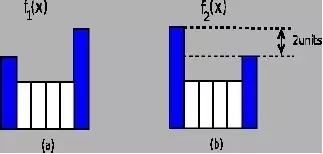
\includegraphics[width=8cm]{images/Wasserstein_distribution.jpg}
                \caption{分布转移示意图}
                \label{fig:Wasserstein距离:分布转移示意图}
                \end{figure}
            % \textcolor[rgb]{1 0 0}{todo:图片:Wasserstein距离:分布转移示意图}
            \begin{lemma}[Lemma4]
            若$\epsilon$是零均值的随机向量,则我们有
            \begin{align*}
            W(P_X,P_{X+\epsilon}) \leqslant V^{\frac{1}{2}}
            \end{align*}
            其中:$V = \mathbb{E}[||\epsilon||_2^2]$是$\epsilon$的方差。
            \end{lemma}
            \begin{Proof}
            令$x\sim P_X$,$y = x+\epsilon$并且$\epsilon$和$x$独立。令$r$为$x,y$的积分域,它有边界$P_X$和$P_{X+\epsilon}$。Therefore
            \begin{align*}
            W(P_X,P_{X+\epsilon})& \leqslant \int ||x-y||_2\mathrm{d}\gamma(x,y)\\
            & = \mathbb{E}_{x\sim P_X}\mathbb{E}_{y\sim x+\epsilon} [||x-y||_2]\\
            &=\mathbb{E}_{x\sim P_X}\mathbb{E}{y\sim x+\epsilon}[||\epsilon||_2]\\
            &=\mathbb{E}_{x\sim P_X}\mathbb{E}_\epsilon [||\epsilon||_2]\\
            &=\mathbb{E}_\epsilon[||\epsilon||_2]\\
            & \leqslant \mathbb{E}_\epsilon[||\epsilon||_2^2]^{\frac{1}{2}} = V^{\frac{1}{2}}
            \end{align*}
            where the last inequality was due to Jensen. $\square$
            \end{Proof}
            引理4表明,一个分布于它添加扰动后的分布的Wasserstein距离能被扰动的标准差bound住。
            \begin{theorem}[Theorem 3.3]
            设$P_r$和$P_g$是任意的两个分布,$\epsilon$是一个零均值,方差为$V$的随机向量。若$P_{r+\epsilon}$和$P_{g+\epsilon}$的支撑集落在直径为$C$的球内,则
            \begin{align*}
            W(P_r,P_g) \leqslant 2 V^{\frac{1}{2}}+2C\sqrt{JSD(P_{r+\epsilon}||P_{g+\epsilon})}
            \end{align*}
            \end{theorem}
            \begin{Proof}
            \begin{align*}
            W(P_r) & \leqslant W(P_r||P_{r+\epsilon})+W(P_{r+\epsilon},P_{g+\epsilon})+W(P_{g+\epsilon},P_g)\\
             & \leqslant 2V^{\frac{1}{2}} + W(P_{r+\epsilon},P_{g+\epsilon})\\
             & \leqslant 2V^{\frac{1}{2}} + C\delta(P_{r+\epsilon},P_{g+\epsilon})\\
             & \leqslant 2V^{-\frac{1}{2}} + C(\delta(P_{r+\epsilon},P_m)+\delta(P_{g+\epsilon},P_m) )\\
             & \leqslant 2V^{\frac{1}{2}} + C \left( \sqrt{\frac{1}{2}KL(P_{r+\epsilon}||P_m)} + \sqrt{\frac{1}{2}KL(P_{g+\epsilon}||P_m)} \right) \\
             & \leqslant 2V^{\frac{1}{2}} + 2C\sqrt{JSD(P_{r+\epsilon}||P_{g+\epsilon})}
            \end{align*}
            \par
            上述推导的过程是:first used the Lemma 4 to bound everything but the middle term as a funtion of $V$. After that, we followed by the fact that $W(P.Q)\leqslant C\delta (P,Q)$with $\delta$ the total variation, which is a popular Lemma arizing from the Kantorovich - Rubinstein duality.After that, we used the reiangular inequality on $\delta$ and $P_m$ the mixture distribution between $P_{g+\epsilon}$ and $P_{r+\epsilon}$. Finally, we used Pinsker's inequality and later the fact that each individual KL is only one of the non-negative summands of the JSD.
            \end{Proof}
            \par
            定理3.3告诉我们一个有趣的事实,上式右边两项均能被控制。第一项可以通过逐步减小噪声来逐步减小;第二项可以通过训练GAN(给D的输入添加噪声)来最小化。
            \par
            作者指出,这种通过给D的输入添加噪声的解决方案具有一大好处,那就是我们不需要再担心训练过程。由于引入了噪声,我们可以训练D直到最优而不会遇到G的梯度消失或者训练不稳定的问题,此时G的梯度可以通过推论3.2给出。加噪方案是针对原始GAN问题的第二点根源提出的,解决了训练不稳定的问题,不需要小心平衡判别器训练的火候,可以放心地把判别器训练到接近最优,但是这种解决方法仍然没能够提供一个衡量训练进程的数值指标。
            \par
            总而言之,上面从理论上研究了GAN训练过程中经常出现的两大问题:G的梯度消失、训练不稳定。并且提出了利用地动距离来衡量$P_r$和$P_g$的相似性、对D的输入引入噪声来解决GAN的两大问题,作者证明了地动距离具有上界,并且上界可以通过有效的措施逐步减小。
            \par
            这可以说是一个临时性的解决方案,作者甚至没有给出实验进行验证。在WGAN\cite{2017.Chen}这篇文章中,作者提出了更完善的解决方案,并且做了实验进行验证。下面我们就来看一下这篇文章。

        \subsubsection{Wasserstein距离的优越性质}
            \paragraph{常见距离}
            Martin Arjovsky在文献\cite{2017.Chen}进一步论述了为什么选择Wasserstein距离(地动距离)。
            设$\mathcal{X}$是一个紧致度量空间,这里讨论的图像空间$[0,1]^d$就是紧致度量空间。用$\Sigma$表示$\mathcal{X}$上的所有博雷尔集,用$\mathrm{Prob}(\mathcal{X})$表示定义在$\mathcal{X}$上的概率度量空间。给定$\mathrm{Prob}(\mathcal{X})$上的两个分布$P_r,P_g$,我们可以定义它们的距离/散度(注意:散度不是距离,它不是对称的。距离和散度都可以用于衡量两个分布的相似程度)
            \begin{enumerate}
            \item 全变差(Total Variation)距离
            \begin{align*}
            \delta(P_r,P_g) = \sup_{A\in \Sigma}|P_r(A)-P_g(A)|
            \end{align*}
            \item KL散度(Kullback-Leibler divergence)
            \begin{align*}
            KL(P_r||P_g) = \int \log \left( \frac{p_r(x)}{p_g(x)} \right) p_r(x)\mathrm{d}\mu(x)
            \end{align*}
            \item JS散度(Jensen - Shannon divergence)
            \begin{align*}
            JS(P_r,P_g) = KL(P_r||P_m) + KL(P_g||P_m)
            \end{align*}
            其中:$P_m = \frac{P_r+P_g}{2}$。
            \item Wasserstein距离/地动距离(Wasserstein/Earth - Mover)
            \begin{align}
            \label{eq:Wasserstein距离}
            W(P_r,P_g) = \inf_{\gamma\in \Pi(P_r,P_g)}\mathbb{E}_{(x,y\sim \gamma)}[||x-y||]
            \end{align}
            其中:$\Pi(P_r,P_g)$表示以$P_r,P_g$为边缘分布的所有联合分布组成的集合。
            \end{enumerate}
            \par
            Wasserstein距离相比KL散度、JS散度的优越性在于,即便两个分布没有重叠,Wasserstein距离仍然能够反映它们的远近。
            \par
            用一个简单的例子来看一下这四种距离/散度是怎么计算的。考虑下图(\ref{fig:2个均匀分布距离示意图})的两个均匀分布
                \begin{figure}[H]
                \centering
                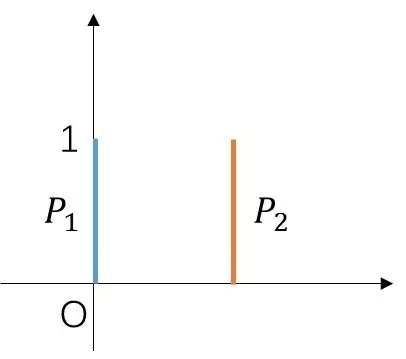
\includegraphics[width=4cm]{images/Two_uniform_distribution_distances.jpg}
                \caption{2个均匀分布距离示意图}
                \label{fig:2个均匀分布距离示意图}
                \end{figure}
            % \textcolor[rgb]{1 0 0}{todo:图片:2个均匀分布距离示意图} \\
            二维平面上,$P_1$是沿着$y$轴的$[0,1]$区间上的均匀分布,$P_2$是沿着$x=0$,在$y$轴的$[0,1]$区间上的均匀分布。简而言之,我们可以把$P_1$和$P_2$看成是两条平行的线段。容易计算
            \begin{align*}
            &\delta(P_1,P_2) =
            \left\{
            \begin{aligned}
            1, \quad \theta \neq 0\\
            0,\quad \theta = 0
            \end{aligned}
            \right.\\
            &KL(P_1||P_2) = KL(P_2||P_1) =
            \left\{
            \begin{aligned}
            +\infty ,\quad \theta \neq 0\\
            0,\quad \theta = 0
            \end{aligned}
            \right.\\
            &JS(P_1,P_2) =
            \left\{
            \begin{aligned}
            \log 2,\quad \theta \neq 0\\
            0,\quad \theta =0
            \end{aligned}
            \right.\\
            &W(P_1,P_2) = |\theta|
            \end{align*}
            \par
            当$\theta \to 0$时,$W\to 0$,然而TV距离、KL散度、JS散度都不收敛。KL散度和JS散度是突变的,要么最大要么最小,而Wasserstein距离却是平滑的,如果我们要用梯度下降法优化$\theta$这个参数,前两者根本提供不了梯度,但Wasserstein距离却可以。类似地,在高维空间中如果两个分布不重叠或者重叠部分可忽略,则KL和JS既反映不了远近,也提供不了梯度,但是Wasserstein却可以提供有意义的梯度。
            更严谨的结论由下面的定理给出。
            \begin{theorem}[Theorem 1]
            设$P_r$是定义在$\mathcal{X}$上的一个固定分布,$z$是定义在$\mathcal{Z}$空间上的随机变量。再设$g:\mathcal{Z}\times R^d\to \mathcal{X}$是一个函数,记为$g_\theta(z)$。记$g_\theta(Z)$的分布为$P_\theta$,则
            \begin{enumerate}
            \item  若$g$关于$\theta$连续,则$W(P_r,P_\theta)$也连续;
            \item 若$g$满足局部Lipschitz条件,局部Lipschitz常数为$L(\theta,z)$,且$\mathbb{E}_{z\sim p(z)}L(\theta,z)< +\infty$,则$W(P_r,P_\theta)$处处连续,且几乎处处可微。
            \end{enumerate}
            \end{theorem}
            \par
            上述两个结论对JS散度和KL散度均不成立。定理1表明,地动距离与JS散度、KL散度相比,具有更好的性质。
            \begin{corollary}[corollary 1]
            设$g_\theta$是任意一个前向传播网络,带有参数$\theta$,并且$p(z)$是关于$z$的先验概率,满足$\mathbb{E}_{z\sim p(z)}||z|| < +\infty$。$g$满足局部Lipschitz条件,局部L常数为$L(\theta,z)$,且$\mathbb{E}_{z\sim p(z)}L(\theta,z)<+\infty$,则$W(P_r,P_\theta)$处处连续,且几乎处处可微。
            \end{corollary}
            \par
            上述推论1(corollary 1)表明,将地动距离作为神经网络的目标函数是可行的。
            \begin{theorem}[Theorem 2]
            设$P$是紧致空间$\mathcal{X}$上的一个分布,并且$(P_n)_{n\in \mathbb{N}}$是$\mathcal{X}$上的一个分布序列,则当$n\rightarrow \infty$时
            \begin{enumerate}
            \item 下面两个命题是等价的
            \begin{enumerate}
            \item $\delta(P_n,P)\to 0$ with $\delta$ the total variation distace;
            \item $JS(P_n,P)\to 0$。
            \end{enumerate}
            \item 下面两个命题是等价的
            \begin{enumerate}
            \item $W(P_n,P)\to 0$.
            \item $P_n$依分布收敛于$P$,$P_n\xrightarrow{D} P$。
            \end{enumerate}
            \item $KL(P_n||P)\to 0$或者$KL(P||P_n)\to 0$能导出结论1.
            \item 结论1能导出结论2.
            \end{enumerate}
            \end{theorem}
            \par
            定理2(Theorem 2)表明,如果分布的支撑集在低维流形上,KL散度、JS散度和TV距离并不是好的loss,而地动(EM)距离则很合适。这启发我们可以用地动距离(EM)来设计loss以替换原来GAN采用的KL散度。


        \subsubsection{从Wasserstein距离到WGAN}
            \par
            采用Wasserstein距离作为loss的GAN称为WassersteinGAN,一般简写为WGAN。直接考虑Wasserstein距离需要算$\inf$,计算是很困难的,因为Wasserstein距离定义(\ref{eq:Wasserstein距离})中的$\inf_{\gamma \sim \Pi (P_r, P_g)}$没法直接求解。考虑它的Kantorovich-Rubinstein对偶形式
            \begin{align*}
            W(P_r,P_\theta) = \sup_{||f||_L \leqslant 1}\mathbb{E}_{x\sim P_r}[f(x)] - \mathbb{E}_{x\sim P_\theta}[f(x)]
            \end{align*}
            其中:$||f||_L \leqslant 1$是所有的1-Lipschitz函数$f:\mathcal{X}\to R$。也就是说,Wasserstein距离实际上需要考虑所有的1-Lipschitz函数。如果我们考虑的是K-Lipschitz函数,这Wasserstein距离变为原来的$K$倍

            \begin{align}
            \label{公式13}
            W(P_r, P_g) = \frac{1}{K} \sup_{||f||_L \leq K} \mathbb{E}_{x \sim P_r} [f(x)] - \mathbb{E}_{x \sim P_g} [f(x)]
            \end{align}
            \par
            式(\ref{公式13})的意思就是在要求函数$f$的Lipschitz常数$||f||_L$不超过$K$的条件下,对所有可能满足条件的$f$取到$\mathbb{E}_{x \sim P_r} [f(x)] - \mathbb{E}_{x \sim P_g} [f(x)]$的上界,然后再除以$K$。特别地,我们可以用一组参数$w$来定义一系列可能的函数$f_w$,此时求解式(\ref{公式13})可以近似变成求解如下形式
            \begin{align}
            \label{公式14}
            K \cdot W(P_r, P_g) \approx \max_{w: |f_w|_L \leq K} \mathbb{E}_{x \sim P_r} [f_w(x)] - \mathbb{E}_{x \sim P_g} [f_w(x)]
            \end{align}
            \par
            可以把$f$用一个带参数$w$的神经网络来表示。由于神经网络的拟合能力足够强大,我们有理由相信,这样定义出来的一系列$f_w$虽然无法囊括所有可能,但是也足以高度近似式(\ref{公式13})要求的那个$\sup_{||f||_L \leq K} $了。
            \par
            最后,还不能忘了满足式(\ref{公式14})中$||f_w||_L \leq K$这个限制。我们其实不关心具体的$K$是多少,只要它不是正无穷就行,因为它只是会使得梯度变大$K$倍,并不会影响梯度的方向。所以作者采取了一个非常简单的做法,就是限制神经网络$f_\theta$的所有参数$w_i$的不超过某个范围$[-c, c]$,比如$w_i \in [- 0.01, 0.01]$。此时关于输入样本$x$的导数$\frac{\partial f_w}{\partial x}$也不会超过某个范围,所以一定存在某个不知道的常数$K$使得$f_w$的局部变动幅度不会超过它,Lipschitz连续条件得以满足。具体在算法实现中,只需要每次更新完$w$后把它clip回这个范围就可以了。
            \par
            到此为止,我们可以构造一个含参数$w$、最后一层不是非线性激活层的判别器网络$f_w$,在限制$w$不超过某个范围的条件下,使得
            \begin{align}
            \label{公式15}
            L = \mathbb{E}_{x \sim P_r} [f_w(x)] - \mathbb{E}_{x \sim P_g} [f_w(x)]
            \end{align}
            尽可能取到最大,此时$L$就会近似真实分布与生成分布之间的Wasserstein距离(忽略常数倍数$K$)。注意原始GAN的判别器做的是真假二分类任务,所以最后一层是sigmoid,但是现在WGAN中的判别器$f_w$做的是近似拟合Wasserstein距离,属于回归任务,所以要把最后一层的sigmoid拿掉。
            \par
            接下来生成器要近似地最小化Wasserstein距离,可以最小化$L$,由于Wasserstein距离的优良性质,我们不需要担心生成器梯度消失的问题。再考虑到L的第一项与生成器无关,就得到了WGAN的两个loss:
            \begin{align}
            \label{公式16,WGAN生成器loss函数}
            - \mathbb{E}_{x \sim P_g} [f_w(x)]
            \end{align}
            和
            \begin{align}
            \label{公式17,WGAN判别器loss函数}
            \mathbb{E}_{x \sim P_g} [f_w(x)]- \mathbb{E}_{x \sim P_r} [f_w(x)]
            \end{align}
            \par
            式(\ref{公式15})是式(\ref{公式17,WGAN判别器loss函数})的反,可以指示训练进程,其数值越小,表示真实分布与生成分布的Wasserstein距离越小,GAN训练得越好。
            \par
            记$G = g_\theta,D = f_w$,则上式(\ref{公式15})写为
            \begin{align*}
            \max_D\  \mathbb{E}_{x\sim P_r}[D(x)] - \mathbb{E}_{z\sim p(z)}[D(G(z))]
            \end{align*}
            我们再次回顾一下原GAN中的目标
            \begin{align*}
            \max_D \mathbb{E}_{x\sim P_r}[\log D(x)] - \mathbb{E}_{z\sim p(z)}[\log (1-D(G(z)))]
            \end{align*}
            可以看到,如果把GAN的目标函数的$\log$去掉,则两者只相差一个常数,也就是说,WGAN在训练的时候与GAN几乎一样,除了loss计算的时候不取对数!Loss function中的对数函数导致了GAN训练的不稳定!
            \begin{theorem}[Theorem 3]
            设$P_r$是任一分布,$P_\theta$是$g_\theta(Z)$的分布,其中$Z$的先验概率密度函数为$p(z)$,$g$满足局部Lipschitz条件,局部Lipschitz常数为$L(\theta,z)$,且$E_{z\sim p(z)} L(\theta,z)<+\infty $,则下述问题存在解$f:\mathcal{X}\to R$
            \begin{align*}
            \max _{||f||_L \leqslant 1} \mathbb{E}_{x\sim P_r}[f(x)] - \mathbb{E}_{x\sim P_\theta }[f(x)]
            \end{align*}
            并且,我们有
            \begin{align*}
            \nabla_\theta W(P_r,P_\theta) = -\mathbb{E}_{z\sim p(z)}[\nabla _\theta f(g_\theta(z))]
            \end{align*}
            when both terms are well-defined
            \end{theorem}
            \par
            定理3(Theorem 3)证明了若D和G的学习能力足够强的话(因此目标函数能够被最大化),WGAN是有解的。改进后相比原始GAN的算法实现流程却只改了四点:
            \begin{enumerate}
            \item 判别器最后一层去掉sigmoid;
            \item 生成器和判别器的loss不取log;
            \item 每次更新判别器的参数之后把它们的绝对值截断到不超过一个固定常数$c$;
            \item 不要用基于动量的优化算法(包括momentum和Adam),推荐RMSProp,SGD也行。
            \end{enumerate}
            \par
            前三点都是从理论分析中得到的,已经介绍完毕;第四点却是作者从实验中发现的,属于trick。作者发现如果使用Adam,判别器的loss有时候会崩掉,当它崩掉时,Adam给出的更新方向与梯度方向夹角的cos值就变成负数,更新方向与梯度方向南辕北辙,这意味着判别器的loss梯度是不稳定的,所以不适合用Adam这类基于动量的优化算法。作者改用RMSProp之后,问题就解决了,因为RMSProp适合梯度不稳定的情况。
        \subsubsection{WGAN程序}
            \par
            WGAN算法伪代码如(\ref{code:WGAN})所示
            \begin{algorithm}[htbp]
                \caption{WGAN,our proposed algorithm. All experiments in the used the default values $\alpha = 0.00005$,$c=0.01$,$m=64$,$n_{critic}=5$}\label{code:WGAN}
                \begin{algorithmic}[1]
                    \State 初始化:学习率$\alpha$,修剪参数$c$;批量大小$m$;循环$n_{critic}$;初始化critic的参数$w_0$,生成器G的参数$\theta_0$。
                    \While {未达到停止准则}
                        \For {$t=1$ to $n_{critic}$}
                            \State 采样$\{x^{(i)}\}_{i=1}^m\sim P_r$;
                            \State 采样$\{z^{(i)}\}_{i=1}^m\sim P_z$;
                            \State
                            \begin{align*}
                            g_w \leftarrow \nabla_w \left[\frac{1}{m}\sum_{i=1}^m f_w(x^{(i)}) - \frac{1}{m}\sum_{i=1}^mf_w(g_\theta(z^{(i)}))\right]
                            \end{align*}
                            \State $w\leftarrow w+\alpha \cdot \mathrm{RMSProp}(w,g_w)$;
                            \State $w\leftarrow \mathrm{clip}(w,-c,c)$
                        \EndFor
                        \State 采样$\{z^{(i)}\}_{i=1}^m\sim P_z$;
                        \State 更新$g_\theta \leftarrow \nabla_\theta\frac{1}{m}\sum_{i=1}^mf_w(g_\theta(z^{(i)}))$
                        \State $\theta \leftarrow \theta - \alpha \cdot \mathrm{RMSProp}(w,g_\theta)$
                    \EndWhile
                \end{algorithmic}
            \end{algorithm}

            \par
            WGAN 源码实现\footnote{https://github.com/martinarjovsky/WassersteinGAN}和
            \footnote{https://github.com/wiseodd/generative-models}。下面给出WGAN的TensorFlow程序
            \begin{lstlisting}[language = Python]
            import tensorflow as tf
            from tensorflow.examples.tutorials.mnist import input_data
            import numpy as np
            import matplotlib.pyplot as plt
            import matplotlib.gridspec as gridspec
            import os
            mb_size = 32
            X_dim = 784
            z_dim = 10
            h_dim = 128
            mnist = input_data.read_data_sets('../../MNIST_data', one_hot=True)
            def plot(samples):
                fig = plt.figure(figsize=(4, 4))
                gs = gridspec.GridSpec(4, 4)
                gs.update(wspace=0.05, hspace=0.05)
                for i, sample in enumerate(samples):
                    ax = plt.subplot(gs[i])
                    plt.axis('off')
                    ax.set_xticklabels([])
                    ax.set_yticklabels([])
                    ax.set_aspect('equal')
                    plt.imshow(sample.reshape(28, 28), cmap='Greys_r')
                return fig
            def xavier_init(size):
                in_dim = size[0]
                xavier_stddev = 1. / tf.sqrt(in_dim / 2.)
                return tf.random_normal(shape=size, stddev=xavier_stddev)
            X = tf.placeholder(tf.float32, shape=[None, X_dim])
            D_W1 = tf.Variable(xavier_init([X_dim, h_dim]))
            D_b1 = tf.Variable(tf.zeros(shape=[h_dim]))
            D_W2 = tf.Variable(xavier_init([h_dim, 1]))
            D_b2 = tf.Variable(tf.zeros(shape=[1]))
            theta_D = [D_W1, D_W2, D_b1, D_b2]
            z = tf.placeholder(tf.float32, shape=[None, z_dim])
            G_W1 = tf.Variable(xavier_init([z_dim, h_dim]))
            G_b1 = tf.Variable(tf.zeros(shape=[h_dim]))
            G_W2 = tf.Variable(xavier_init([h_dim, X_dim]))
            G_b2 = tf.Variable(tf.zeros(shape=[X_dim]))
            theta_G = [G_W1, G_W2, G_b1, G_b2]
            def sample_z(m, n):
                return np.random.uniform(-1., 1., size=[m, n])
            def generator(z):
                G_h1 = tf.nn.relu(tf.matmul(z, G_W1) + G_b1)
                G_log_prob = tf.matmul(G_h1, G_W2) + G_b2
                G_prob = tf.nn.sigmoid(G_log_prob)
                return G_prob
            def discriminator(x):
                D_h1 = tf.nn.relu(tf.matmul(x, D_W1) + D_b1)
                out = tf.matmul(D_h1, D_W2) + D_b2
                return out
            G_sample = generator(z)
            D_real = discriminator(X)
            D_fake = discriminator(G_sample)
            D_loss = tf.reduce_mean(D_real) - tf.reduce_mean(D_fake)
            G_loss = -tf.reduce_mean(D_fake)
            D_solver = (tf.train.RMSPropOptimizer(learning_rate=1e-4)
                        .minimize(-D_loss, var_list=theta_D))
            G_solver = (tf.train.RMSPropOptimizer(learning_rate=1e-4)
                        .minimize(G_loss, var_list=theta_G))
            clip_D = [p.assign(tf.clip_by_value(p, -0.01, 0.01)) for p in theta_D]
            sess = tf.Session()
            sess.run(tf.global_variables_initializer())
            if not os.path.exists('out/'):
                os.makedirs('out/')
            i = 0
            for it in range(1000000):
                for _ in range(5):
                    X_mb, _ = mnist.train.next_batch(mb_size)
                    _, D_loss_curr, _ = sess.run(
                        [D_solver, D_loss, clip_D],
                        feed_dict={X: X_mb, z: sample_z(mb_size, z_dim)}
                    )
                _, G_loss_curr = sess.run(
                    [G_solver, G_loss],
                    feed_dict={z: sample_z(mb_size, z_dim)}
                )
                if it % 100 == 0:
                    print('Iter: {}; D loss: {:.4}; G_loss: {:.4}'
                          .format(it, D_loss_curr, G_loss_curr))
                    if it % 1000 == 0:
                        samples = sess.run(G_sample, feed_dict={z: sample_z(16, z_dim)})

                        fig = plot(samples)
                        plt.savefig('out/{}.png'
                                    .format(str(i).zfill(3)), bbox_inches='tight')
                        i += 1
            plt.close(fig)
            \end{lstlisting}
            \par
            WGAN实验:对WGAN作者做了不少实验验证,下面只提比较重要的三点。第一,判别器所近似的Wasserstein距离与生成器的生成图片质量高度相关。Wasserstein距离越小,G产生的图像质量就越高。先前的GAN由于训练不稳定,我们很难通过loss去判断G产生的质量(先前的GAN的loss大小并不能表明产生图像质量的高低),如下图(\ref{fig:Wasserstein距离与生成器的生成图片质量})所示
                \begin{figure}[H]
                \centering
                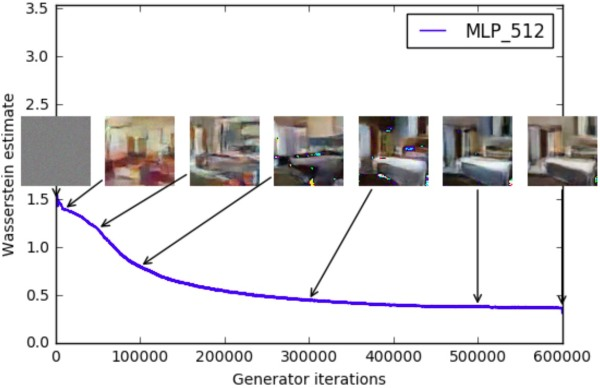
\includegraphics[width=8cm]{images/Wasserstein_picture.jpg}
                \caption{Wasserstein距离与生成器的生成图片质量}
                \label{fig:Wasserstein距离与生成器的生成图片质量}
                \end{figure}
            % \textcolor[rgb]{1 0 0}{todo:图片:Wasserstein距离与生成器的生成图片质量}\\
            第二,WGAN如果用类似DCGAN架构,生成图片的效果与DCGAN差不多,如图(\ref{fig:WAGN和DCGAN对比图})所示
                \begin{figure}[H]
                \centering
                
\includegraphics[width=12cm]{images/WAGN_and_DCGAN.jpg}
                \caption{WAGN和DCGAN对比图}
                \label{fig:WAGN和DCGAN对比图}
                \end{figure}
            % \textcolor[rgb]{1 0 0}{todo:图片:WAGN和DCGAN对比图}\\
            但是厉害的地方在于WGAN不用DCGAN各种特殊的架构设计也能做到不错的效果,如果一起拿掉Batch Normalization的话,DCGAN就崩了而WGAN不会,如图(\ref{fig:DCGAN去掉BN的崩溃})所示
                \begin{figure}[H]
                \centering
                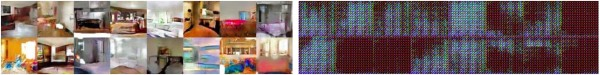
\includegraphics[width=12cm]{images/DCGAN_remove_BN.jpg}
                \caption{DCGAN去掉BN的崩溃}
                \label{fig:DCGAN去掉BN的崩溃}
                \end{figure}
            % \textcolor[rgb]{1 0 0}{todo:图片:DCGAN去掉BN的崩溃}\\
            如果WGAN和原始GAN都使用多层全连接网络(MLP),不用CNN,WGAN质量会变差些,但是原始GAN不仅质量变得更差,而且还出现了collapse mode,即多样性不足,如图(\ref{fig:WGAN和DCGAN去掉CNN对比结果})所示
                \begin{figure}[H]
                \centering
                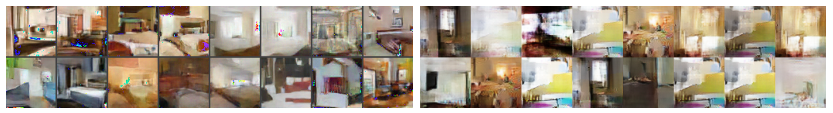
\includegraphics[width=12cm]{images/WGAN_and_DCGAN_remove_CNN.png}
                \caption{WGAN和DCGAN去掉CNN对比结果}
                \label{fig:WGAN和DCGAN去掉CNN对比结果}
                \end{figure}
            % \textcolor[rgb]{1 0 0}{todo:图片:WGAN和DCGAN去掉CNN对比结果}\\
            第三,在所有WGAN的实验中未观察到collapse mode,作者也只说应该是解决了。
            % \par
            % 最后补充一点论文没提到,但是我个人觉得比较微妙的问题。判别器所近似的Wasserstein距离能够用来指示单次训练中的训练进程,这个没错;接着作者又说它可以用于比较多次训练进程,指引调参,我倒是觉得需要小心些。比如说我下次训练时改了判别器的层数、节点数等超参,判别器的拟合能力就必然有所波动,再比如说我下次训练时改了生成器两次迭代之间,判别器的迭代次数,这两种常见的变动都会使得Wasserstein距离的拟合误差就与上次不一样。那么这个拟合误差的变动究竟有多大,或者说不同的人做实验时判别器的拟合能力或迭代次数相差实在太大,那它们之间还能不能直接比较上述指标,我都是存疑的。
            % 评论区的知友$\@ Minjie Xu $进一步指出,相比于判别器迭代次数的改变,对判别器架构超参的改变会直接影响到对应的Lipschitz常数$K$,进而改变近似Wasserstein距离的倍数,前后两轮训练的指标就肯定不能比较了,这是需要在实际应用中注意的。对此我想到了一个工程化的解决方式,不是很优雅:取同样一对生成分布和真实分布,让前后两个不同架构的判别器各自拟合到收敛,看收敛到的指标差多少倍,可以近似认为是后面的$K_2$相对前面$K_1$的变化倍数,于是就可以用这个变化倍数校正前后两轮训练的指标。


            % \subsubsection{总结}
            %     \par
            %     WGAN前作分析了Ian Goodfellow提出的原始GAN两种形式各自的问题,第一种形式等价在最优判别器下等价于最小化生成分布与真实分布之间的JS散度,由于随机生成分布很难与真实分布有不可忽略的重叠以及JS散度的突变特性,使得生成器面临梯度消失的问题;第二种形式在最优判别器下等价于既要最小化生成分布与真实分布直接的KL散度,又要最大化其JS散度,相互矛盾,导致梯度不稳定,而且KL散度的不对称性使得生成器宁可丧失多样性也不愿丧失准确性,导致collapse mode现象。
            %     \par
            %     WGAN前作针对分布重叠问题提出了一个过渡解决方案,通过对生成样本和真实样本加噪声使得两个分布产生重叠,理论上可以解决训练不稳定的问题,可以放心训练判别器到接近最优,但是未能提供一个指示训练进程的可靠指标,也未做实验验证。
            %     \par
            %     WGAN本作引入了Wasserstein距离,由于它相对KL散度与JS散度具有优越的平滑特性,理论上可以解决梯度消失问题。接着通过数学变换将Wasserstein距离写成可求解的形式,利用一个参数数值范围受限的判别器神经网络来最大化这个形式,就可以近似Wasserstein距离。在此近似最优判别器下优化生成器使得Wasserstein距离缩小,就能有效拉近生成分布与真实分布。WGAN既解决了训练不稳定的问题,也提供了一个可靠的训练进程指标,而且该指标确实与生成样本的质量高度相关。作者对WGAN进行了实验验证。

    \subsection{Improved WGAN}
        \subsubsection{问题分析}
            \par
            WGAN虽然克服了GAN梯度消失等问题,但是在某些设置下,WGAN生成的样本仍然是低质量的,甚至不收敛。文献\cite{2017.Ishaan}的作者发现,WGAN强行使critic是lipschitz连续的权重修剪技术(weight clipping)会导致WGAN失败。为了强行使用lipschitz连续,作者在improved WGAN中设置了一个交替的方法:惩罚critic梯度的范数。相对而言,Improved WGAN有更快的收敛速度和更高的图像质量。
            \par
            WGAN的价值函数是通过 Kantorovich-Rubinstein对偶建立的
            \begin{align*}
            \min_G\ \max_{D\in \mathcal{D}} \ \mathbb{E}_{x\sim p_r}[D(x)] - \mathbb{E}_{\tilde{x}\sim p_g}[D(\tilde{x})]
            \end{align*}
            其中:$\mathcal{D}$是一个1-lipschitz函数集,$\tilde{x} = G(z),z\sim p_z$。一个公开的问题是如何有效的对critic进行lipschitz约束? Arjovsky在WGAN中使用了权重裁剪技术,使权重在$[-c,c]$范围内(每当更新完一次判别器的参数之后,就检查判别器的所有参数的绝对值有没有超过一个阈值。通过在训练过程中保证判别器的所有参数有界,就保证了判别器不能对两个略微不同的样本给出天差地别的分数值,从而间接实现了Lipschitz限制)。
            \par
            如果在Kantorovich-Rubinstein对偶$D^*$下,最优的critic是可微的,并且$x$是生成分布$p_g$的一个样本,那么,存在一个$p_r$中的点$y$,$D^*$的梯度在所有点$x_t = (1-t)x+ty$直接通向$y$,即
            \begin{align*}
            \nabla D^*(x_t) = \frac{y-x_t}{||y-x_t||}
            \end{align*}
            这意味着最佳WGAN critic的梯度范数为1(almost everywhere $p_r$ and $p_g$)。作者发现WGAN的优化通常是困难的,即便当优化成功时,critic也可能会有比较粗糙的值。下面,我们将展示这些问题及它们的影响(weight clipping的实现方式存在两个严重问题)。
            \par
            实验表明,修剪每一个权重或者修剪权重的1阶范数、2阶范数都会导致相同的问题,这有可能是因为clip“损伤”了WGAN的训练。但是,我们不能声称每一次训练都有问题,特别是当WGAN权重剪枝和batch normalization技术一起使用的时候。有些时候,BN是有用的,在某些时候,特别是深度网络时,优化仍然困难。在Improved WGAN中没有BN的WGAN仍可以成功训练。
            \par
            优化带权重约束的critic相当于优化所有k-lipschitz函数的一个小子集。作者发现,这会导致许多问题,即便当优化任务收敛后,critic也可能收敛到一个非常差的情况。最优的critic(在WGAN损失函数下)的梯度范数为1,然而在权重修剪约束下,大多数网络在学习简单函数时,只能够达到的梯度范数为$k$。因此,通过权重修剪来达到k-lipschitz约束会使critic变成简单函数。例如在权重修剪下,最优critic可能包含许多重复的隐含神经元,忽略网络中的对称性,这最终被汇总来最大化the out 的最终比例。这种策略在最大化$p_r$和$p_g$散度时可能是最优的,但是这会导致在训练G时缺失有价值的梯度。
            \par
            为了证明这一点,我们训练WGAN critic(clipping)来优化3个实验分布:保持生成分布$p_g$固定,在真实分布$p_r$中添加单位方差的高斯噪声,在图(\ref{fig:critics的价值曲面})中给出critics的价值曲面
                \begin{figure}[H]
                \centering
                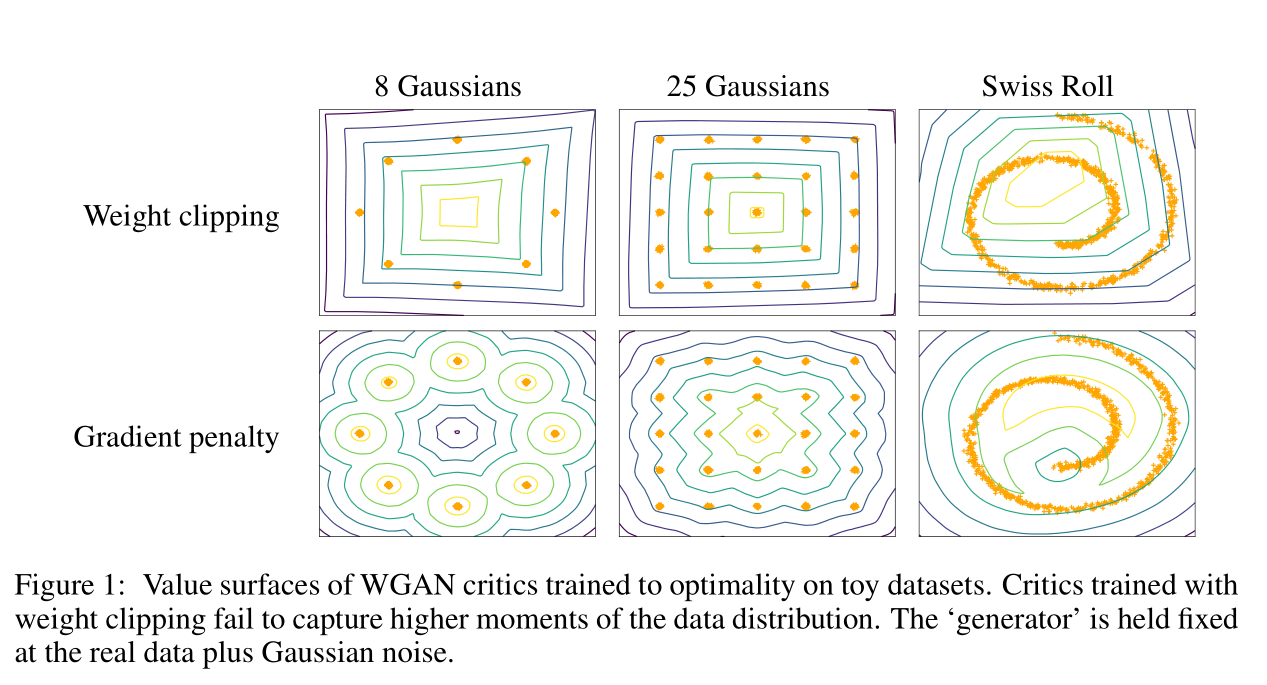
\includegraphics[width=10cm]{images/Critics_of_value_of_the_surface.jpg}
                \caption{critics的价值曲面}
                \label{fig:critics的价值曲面}
                \end{figure}
            % \textcolor[rgb]{1 0 0}{todo:图片:critics的价值曲面}\\
            注意,在Improved WGAN的critic中忽略了BN。在3种实验分布下,通过权重修剪训练的critics忽略了数据分布的高阶矩,并且非常简单的接近最优函数。相比之下,Improved WGAN没有这种问题。
            \par
            如果权重被约束的太小,前层的反向传播带来的梯度会消失。另一方面,如果权重被约束的太大,网络会发生梯度爆炸。这是因为Weight clipping独立地限制每一个网络参数的取值范围,在这种情况下,最优的策略就是尽可能让所有参数走极端,要么取最大值要么取最小值!为了验证这一点,作者统计了经过充分训练的判别器中所有网络参数的数值分布,在图(\ref{fig:WGAN梯度消失和爆炸})(b)左图中展示了这一情况。这样带来的结果就是,判别器会非常倾向于学习一个简单的映射函数(想想看,几乎所有参数都是$\pm0.01$,这可以直接视为一个二值神经网络)。判别器没能充分利用自身的模型能力,经过它回传给生成器的梯度也会跟着变差。
                \begin{figure}[H]
                \centering
                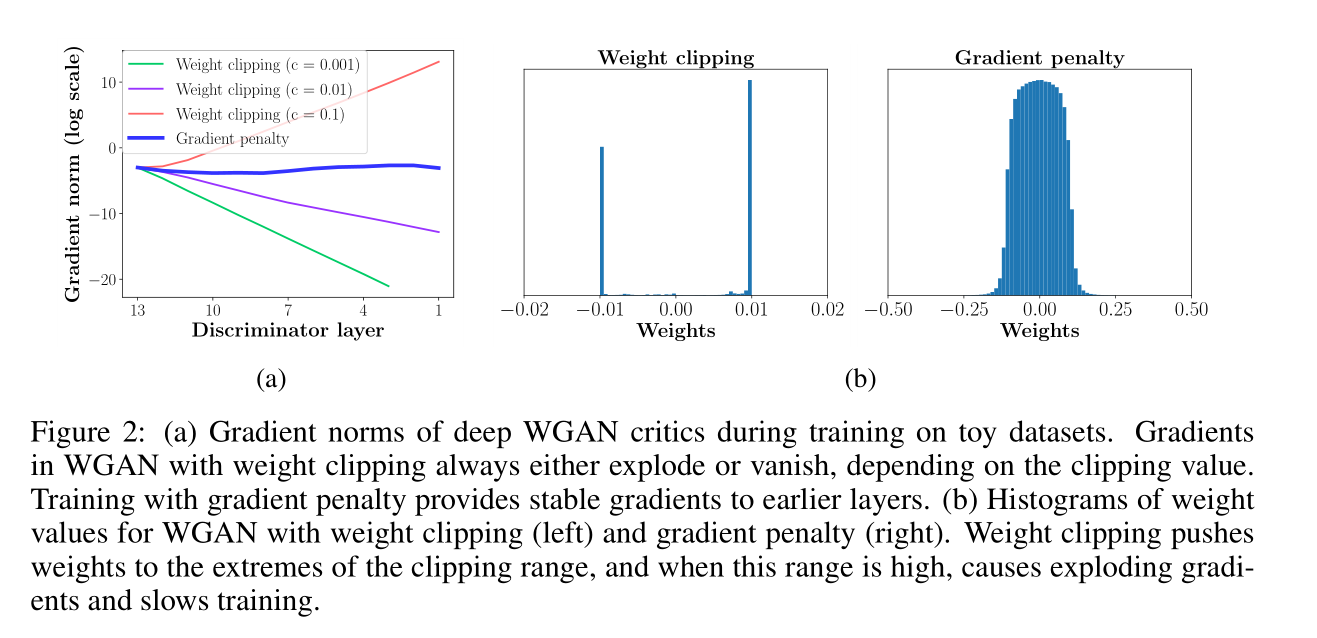
\includegraphics[width=14cm]{images/WGAN_grandient_boom.jpg}
                \caption{WGAN梯度消失和爆炸}
                \label{fig:WGAN梯度消失和爆炸}
                \end{figure}
            % \textcolor[rgb]{1 0 0}{todo:图片:WGAN梯度消失和爆炸}\\
            \par
            为了证明基于权重裁剪的WGAN会发生梯度消失和爆炸,我们在 Swiss Roll实验分布上训练WGAN。并且设置权重修剪参数$c$为$[10^{-1},10^{-2},10^{-3}]$,并绘制critic loss的梯度的模。WGAN中的critic和G都是12-层depReLuMLPs,并且没有BN。在图(\ref{fig:WGAN梯度消失和爆炸})(a)中,横轴代表判别器从低到高第几层,纵轴代表梯度回传到这一层之后的尺度大小(注意纵轴是对数刻度),c是clipping threshold。结果表明:对于每个$c$,梯度会指数增长或减小,因为我们在网络中移动更远。
            \par
            在WGAN中使用BN技术,梯度消失或爆炸问题可能会有所减缓。然而,即使使用BN,非常deep WGAN critics 也经常获得坏的情况,甚至学习失败。
        \subsubsection{梯度惩罚}
            \par
            前面提到,Lipschitz限制是要求判别器的梯度不超过$K$,那我们何不直接设置一个额外的loss项来体现这一点呢?比如
            \begin{align*}
            ReLU(||\nabla_x D(x)||_p-K)
            \end{align*}
            不过,既然判别器希望尽可能拉大真假样本的分布差距,那自然是希望梯度越大越好,变化幅度越大越好,所以判别器在充分训练之后,其梯度norm其实就会是在$K$附近。知道了这一点,我们可以把上面的loss改成要求梯度norm离$K$越近越好,效果是类似
            \begin{align*}
            [||\nabla_x D(x)||_p-K]^2
            \end{align*}
            前面提到过最佳WGAN critic的梯度范数为1(almost everywhere $p_r$ and $p_g$)。我们将$K$设置为1,将上述目标和WGAN原来critic的目标loss加权合并,得到新的critic loss
            \begin{align*}
            L_{critic} = \mathbb{E}_{\tilde{x}\sim p_g}[D(\tilde{x})] - \mathbb{E}_{x\sim p_r}[D(x)] + \lambda \mathbb{E}_{x\sim p_{x}}[(||\nabla_{x}D(x)||_2 - 1)^2]
            \end{align*}
            \par
            上面的目标中有些个问题,3个loss项都是期望的形式,在实现上要变成采样的形式。前面两个期望的采样是一般的,第一个期望是从真样本集里面采,第二个期望是从生成器的噪声输入分布采样后,再由生成器映射到样本空间。可是第三个分布要求我们在整个样本空间$P_x$上采样,这变得非常棘手。由于维度灾难问题,如果要通过采样的方式在图片或自然语言这样的高维样本空间中估计期望值,所需样本量是指数级的,实际上没法做到。作者提出,其实我们没必要在整个样本空间上施加Lipschitz限制,只要重点抓住生成样本集中区域、真实样本集中区域以及夹在它们中间的区域就行了。具体来说,我们先随机采一对真假样本,还有一个0-1的随机数:
            \begin{align*}
            \epsilon \sim U[0,1],\quad x\sim p_r, \quad \tilde{x}\sim p_g
            \end{align*}
            然后在$ x_r $和$ x_g $的连线上随机插值采样
            \begin{align*}
            \hat{x} = \epsilon x+(1-\epsilon)\tilde{x}
            \end{align*}
            定义$\tilde{x}$的分布为$p_{\tilde{x}}$,并且$\hat{x}$是$p_r,p_g$的线性采样样本。最终得到Imoroved WGAN的loss
            \begin{align*}
            L_{critic} = \mathbb{E}_{\tilde{x}\sim p_g}[D(\tilde{x})] - \mathbb{E}_{x\sim p_r}[D(x)] + \lambda \mathbb{E}_{\hat{x}\sim p_{\hat{x}}}[(||\nabla_{\tilde{x}}D(\tilde{x})||_2 - 1)^2]
            \end{align*}
            \par
            在$\lambda$较大的情况下,我们构建的最优critic仍然是Kantorovich-Rubinstein对偶下的最优critic。因此,给定critic足够的能力,G的代价函数仍能回复真实的Wasserstein距离,这个在原始剪枝WGAN中不是必然发生的。梯度部分$||\nabla_{\tilde{x}}D(\tilde{x})||_2$是无参数D关于点$\tilde{x}$的梯度。
            \par
            超参数$\lambda$设置为10。许多GAN在G和D中都采用了BN技术,但在 Improved WGAN中,BN不适用,这是由于我们是对每个样本独立地施加梯度惩罚,判别器的模型架构中不能使用Batch Normalization,因为它会引入同个batch中不同样本的相互依赖关系。如果需要的话,可以选择其他normalization方法,如Layer Normalization、Weight Normalization和Instance Normalization,这些方法就不会引入样本之间的依赖,这里推荐Layer Normalization。

        \subsubsection{Improved WGAN程序}
            \par
            Mali GAN的伪代码如(\ref{code:Mali GAN})所示
            \begin{algorithm}[htbp]
                \caption{WGAN with gradient penalty.We use default values of $\lambda = 10$,$n_{critic} = 5$,$\alpha = 0.0001$,$\beta_1=0.5$,$\beta_2 = 0.9$.}
                \begin{algorithmic}[1]
                    \State 初始化:梯度约束的超参数$\lambda$;critic的循环次数$n_{critic}$;迭代数$t$,$t_{max}$;判别器训练次数$k$;批量大小$m$;Adam的超参数$\alpha,\beta_1,\beta_2$。
                    \For {$t=1,2,\dots,t_{max}$}
                        \For {$k = 1,\dots,n_{critic}$ }
                            \For {$i = 1,\dots,m$}
                                \State Sample real data $x\sim p_r$, latent variable $z\sim p_z$,a random number $\epsilon \sim U[0,1]$。
                                \State $\tilde{x} \leftarrow G_\theta(z)$
                                \State $\hat{x} \leftarrow \epsilon x+(1-\epsilon)\tilde{x}$
                                \State $L^{(i)} \leftarrow D_w(\tilde{x}) - D_w(x) +\lambda(||\nabla_{\hat{x}}D_w(\hat{x})||_2 - 1)^2 $
                            \EndFor
                            \State $w \leftarrow Adam(\nabla_w\frac{1}{m}\sum_{i=1}^m L^{(i)},w,\alpha,\beta_1,\beta_2)$
                        \EndFor
                        \State Sample a batch of latent variables $\{z^{(i)}\}_{i=1}^m \sim p(z)$
                        \State $\theta \leftarrow Adam(\nabla_w\frac{1}{m}\sum_{i=1}^m -D_w(G_\theta(z)),\theta,\alpha,\beta_1,\beta_2)$
                    \EndFor
                \end{algorithmic}
            \end{algorithm}
            \par
            Improved WGAN的TensorFlow程序如下
            \begin{lstlisting}[language = Python]
            import tensorflow as tf
            from tensorflow.examples.tutorials.mnist import input_data
            import numpy as np
            import matplotlib.pyplot as plt
            import matplotlib.gridspec as gridspec
            import os
            mb_size = 32
            X_dim = 784
            z_dim = 10
            h_dim = 128
            lam = 10
            n_disc = 5
            lr = 1e-4
            mnist = input_data.read_data_sets('../../MNIST_data', one_hot=True)
            def plot(samples):
                fig = plt.figure(figsize=(4, 4))
                gs = gridspec.GridSpec(4, 4)
                gs.update(wspace=0.05, hspace=0.05)
                for i, sample in enumerate(samples):
                    ax = plt.subplot(gs[i])
                    plt.axis('off')
                    ax.set_xticklabels([])
                    ax.set_yticklabels([])
                    ax.set_aspect('equal')
                    plt.imshow(sample.reshape(28, 28), cmap='Greys_r')
                return fig
            def xavier_init(size):
                in_dim = size[0]
                xavier_stddev = 1. / tf.sqrt(in_dim / 2.)
                return tf.random_normal(shape=size, stddev=xavier_stddev)
            X = tf.placeholder(tf.float32, shape=[None, X_dim])
            D_W1 = tf.Variable(xavier_init([X_dim, h_dim]))
            D_b1 = tf.Variable(tf.zeros(shape=[h_dim]))
            D_W2 = tf.Variable(xavier_init([h_dim, 1]))
            D_b2 = tf.Variable(tf.zeros(shape=[1]))
            theta_D = [D_W1, D_W2, D_b1, D_b2]
            z = tf.placeholder(tf.float32, shape=[None, z_dim])
            G_W1 = tf.Variable(xavier_init([z_dim, h_dim]))
            G_b1 = tf.Variable(tf.zeros(shape=[h_dim]))
            G_W2 = tf.Variable(xavier_init([h_dim, X_dim]))
            G_b2 = tf.Variable(tf.zeros(shape=[X_dim]))
            theta_G = [G_W1, G_W2, G_b1, G_b2]
            def sample_z(m, n):
                return np.random.uniform(-1., 1., size=[m, n])
            def G(z):
                G_h1 = tf.nn.relu(tf.matmul(z, G_W1) + G_b1)
                G_log_prob = tf.matmul(G_h1, G_W2) + G_b2
                G_prob = tf.nn.sigmoid(G_log_prob)
                return G_prob
            def D(X):
                D_h1 = tf.nn.relu(tf.matmul(X, D_W1) + D_b1)
                out = tf.matmul(D_h1, D_W2) + D_b2
                return out
            G_sample = G(z)
            D_real = D(X)
            D_fake = D(G_sample)
            eps = tf.random_uniform([mb_size, 1], minval=0., maxval=1.)
            X_inter = eps*X + (1. - eps)*G_sample
            grad = tf.gradients(D(X_inter), [X_inter])[0]
            grad_norm = tf.sqrt(tf.reduce_sum((grad)**2, axis=1))
            grad_pen = lam * tf.reduce_mean(grad_norm - 1.)**2
            D_loss = tf.reduce_mean(D_fake) - tf.reduce_mean(D_real) + grad_pen
            G_loss = -tf.reduce_mean(D_fake)
            D_solver = (tf.train.AdamOptimizer(learning_rate=lr, beta1=0.5)
                        .minimize(D_loss, var_list=theta_D))
            G_solver = (tf.train.AdamOptimizer(learning_rate=lr, beta1=0.5)
                        .minimize(G_loss, var_list=theta_G))
            sess = tf.Session()
            sess.run(tf.global_variables_initializer())
            if not os.path.exists('out/'):
                os.makedirs('out/')
            i = 0
            for it in range(1000000):
                for _ in range(n_disc):
                    X_mb, _ = mnist.train.next_batch(mb_size)
                    _, D_loss_curr = sess.run(
                        [D_solver, D_loss],
                        feed_dict={X: X_mb, z: sample_z(mb_size, z_dim)}
                    )
                _, G_loss_curr = sess.run(
                    [G_solver, G_loss],
                    feed_dict={z: sample_z(mb_size, z_dim)}
                )
                if it % 1000 == 0:
                    print('Iter: {}; D loss: {:.4}; G_loss: {:.4}'
                          .format(it, D_loss_curr, G_loss_curr))
                    if it % 1000 == 0:
                        samples = sess.run(G_sample, feed_dict={z: sample_z(16, z_dim)})
                        fig = plot(samples)
                        plt.savefig('out/{}.png'
                                    .format(str(i).zfill(3)), bbox_inches='tight')
                        i += 1
            plt.close(fig)
            \end{lstlisting}
            \par
            Improved WGAN和clipping WGAN等在CIFAR-10上收敛速度的比较如图(\ref{fig:Improved WGAN的收敛速度})所示
                \begin{figure}[H]
                \centering
                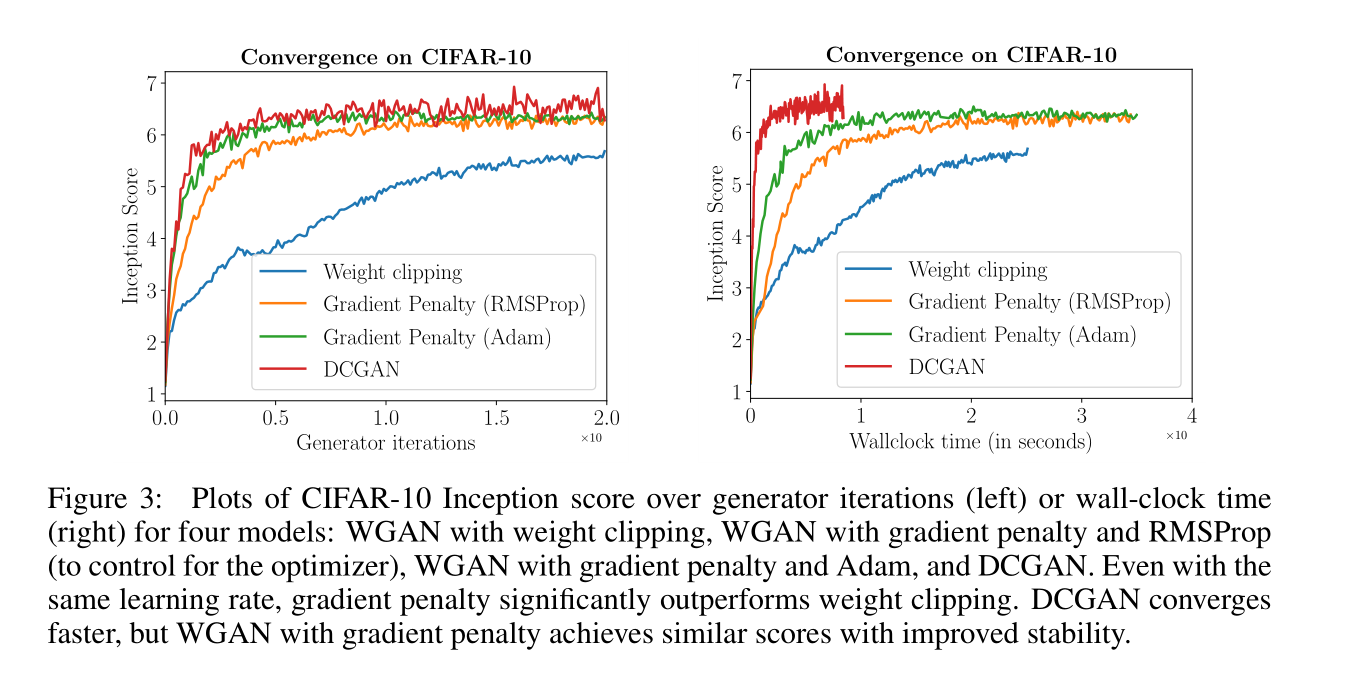
\includegraphics[width=12cm]{images/Improved_WGAN.jpg}
                \caption{Improved WGAN的收敛速度}
                \label{fig:Improved WGAN的收敛速度}
                \end{figure}
            % \textcolor[rgb]{1 0 0}{todo:图片:Improved WGAN的收敛速度}

    \subsection{Loss Sensitive GAN}
        \subsubsection{LS-GAN模型建立}
            \par
            在损失敏感生成对抗网络(LS-GAN)中,我们放弃学习一个判别器D ,而是设置一个损失函数$L_\theta(x)$,并且假设真实样本$x\sim P_r$有小的损失,假样本$x = G(z),z\sim p_z$有大的损失。对于一个给定的$G_\phi$,我们的目标是求$L_\theta$(即$\theta$)使得
            \begin{align*}
            \min_\theta \ \mathbb{E}_{x\sim p_r}L_\theta(x) - \mathbb{E}_{z\sim p_z}L_\theta(G_\phi(z))
            \end{align*}
            \par
            要求真假样本的损失在一定范围内,可以设置如下约束(constraint)
            \begin{align*}
            L_\theta(x)  \leqslant L_\theta(G_\phi(z)) - \Delta(x,G_\phi(z))
            \end{align*}
            其中:$\Delta(x,G_\phi(z))$表示$x$和$G_\phi(z)$之间的不同。现在引入松弛变量$\xi_{x,z}$
            \begin{align*}
            & L_\theta(x) - \xi_{x,z} \leqslant L_\theta(G_\phi(z)) - \Delta(x,G_\phi(z))\\
            & \xi_{x,z} \geqslant 0
            \end{align*}
            当$G_\phi(z)$违反约束时,$\xi_{x,z}$可能是非0的。对于一个给定的$G_\phi$,参数$\theta$的损失函数的训练目标为
            \begin{align*}
            &\min_\theta \ \mathbb{E}_{x\sim p_r} L_\theta(x) + \lambda \mathbb{E}_{x\sim p_r,z\sim p_z} \xi_{x,z}\\
            &s.t. \left\{
            \begin{aligned}
            & L_\theta(x) - \xi_{x,z}  \leqslant L_\theta(G_\phi(z)) - \Delta(x,G_\phi(z))\\
            & \xi_{x,z} \geqslant 0
            \end{aligned}
            \right.
            \end{align*}
            其中:$\lambda$是权重参数。目标中的第一项是真实样本损失最小,第二项是违反约束造成的损失的期望$\mathbb{E} \xi_{x,z}$最小。不失为一般性,我们要求损失函数是非正的,后面将会指出,在某些情况下,非正要求可以去掉。
            \par
            在给定最优损失$L_{\theta^*}$后,对生成器G而言,目标为
            \begin{align*}
            \min_\phi \ \mathbb{E}_{z\sim p_z} L_{\theta^*}(G_\phi(z))
            \end{align*}
            $L_\theta,G_\phi$仍然是交替优化的,最优参数$(\theta^*,\phi^*)$的优化过程为:\ding{172}对$\theta$的优化是在固定$\phi^*$的基础上,求
            \begin{align*}
            \min _\theta S(\theta,\phi^*) = \mathbb{E}_{x\sim p_r}L_\theta(x) + \lambda \mathbb{E}_{x\sim p_r,z\sim p_z} (\Delta(x,G(z))+L_\theta(x)-L_\theta(G(z)))_+
            \end{align*}
            其中:$(a)_+ = \max(a,0)$。
            \par
            \ding{173}对$\phi$的优化是在固定$\theta^*$的基础上,求
            \begin{align*}
            \min _\phi \ T(\theta^*,\phi) = \mathbb{E}_{z\sim p_z}L_{\theta^*}(G(z))
            \end{align*}
            注意到,当假样本$G(z)$的损失和真样本$x$的损失在约束范围内,即$L_\theta(x) - L_\theta(G(z))+\Delta (x,G(z))<0$时,$S(\theta,\phi^*)$第二项的损失为0。这使得当生成样本和真实样本很接近时,我们不必要求他们的$L$函数非得有一个固定间隔,因为这个时候生成的样本已经非常好了。这样LS-GAN就可以集中力量提高那些距离真实样本还很远,真实度不那么高的样本,这样就可以更合理的使用LS-GAN的建模能力。在后面,一旦限定了建模能力后,不用再担心模型的生成能力有损失了,这个我们称“按需分配”。图(\ref{fig:LSGAN-figure1})阐述了LS-GAN背后的“按需分配”的想法。
                \begin{figure}[H]
                \centering
                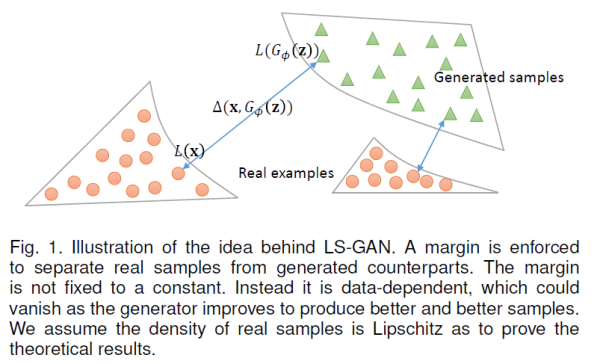
\includegraphics[width=10cm]{images/LSGAN-figure1.jpg}
                \caption{LSGAN-figure1}
                \label{fig:LSGAN-figure1}
                \end{figure}
            % \textcolor[rgb]{1 0 0}{todo:图片:LSGAN-figure1}\\
            边界(magin)是为了区分真假样本,它不是一个固定的常数,它依赖于数据。当生成器生成越来越好的样本时,它会消失。假设真实密度函数$p_r$是lipschitz的,以便于证明结论。
            \par
            设$(\theta^*,\phi^*)$是上面优化问题的纳什均衡,我们可以得到,当$\lambda\to \infty$时,由$G_{\phi^*}$得到的密度$p_{G^*}$将收敛到真实分布$p_r$。为了证明这个结论,先进行如下定义
            \begin{definition}[Lipschitz 函数]
            对于任意的两个样本$x,z$,称损失函数$F(x)$是Lipschitz连续的,如果
            \begin{align*}
            |F(x) - F(z)| \leqslant k \Delta(x,z)
            \end{align*}
            其中:$k$为lipschitz常数,$k<\infty$;$\Delta$为距离度量。
            \end{definition}
            \par
            先将LS-GAN要建模的样本分布$p_r$限定在lipschitz密度上,即
            \begin{Assumption}[1]
            数据密度$p_r$有劲支撑集,且是Lipschitz连续的。
            \end{Assumption}
            \par
            对于Lipschitz密度,简言之,Lipschitz密度就是要求$p_r$不能变化的太快,密度的变化随着样本的变化不能无限的大,要有个度。不过这个都可以非常大,只要不是无限大就好。这个假设还是很弱的,大部分分布都满足之,比如:我们将一个图像调的稍微亮一些,它看上去仍然应该是真实的图像。在真实图像中,密度在lipschitz假设下不应该有突然的、剧烈的变化。
            \begin{lemma}[1]
            在假设1下,给定一个纳什均衡$(\theta^*,\phi^*)$,并且$p_{G^*}$是lipschitz连续的,有
            \begin{align*}
            \int_x|p_r(x) - p_{G^*}(x)|\mathrm{d}x \leqslant \frac{2}{\lambda}
            \end{align*}
            因此,当$\lambda\to \infty$时,$p_{G^*}$收敛到$p_r$。
            \end{lemma}
            \par
            在证明引理1之前,先给出如下引理
            \begin{lemma}[4]
            对于2个概率分布$p(x)$和$q(x)$,如果$p(x) \geqslant \eta q(x)$ a.e (almost everywhere),有
            \begin{align*}
            \int_x|p(x) - q(x)|\mathrm{d}x \leqslant \frac{2(1-\eta)}{\eta}
            \end{align*}
            其中:$\eta\in (0,1]$。
            \end{lemma}
            \begin{Proof}
            我们有如下等式和不等式
            \begin{align*}
            & \int_x|p(x) - q(x)|\mathrm{d}x\\
            ={}&\int_x\mathbbm{1}_{[p(x)\geqslant q(x)]}(p(x)-q(x))\mathrm{d}x+\int_x \mathbbm{1}_{[p(x)<q(x)]}(q(x)-p(x))\mathrm{d}x\\
            ={}& \int_x \left( 1-\mathbbm{1}_{[p(x)<q(x)]} \right) (p(x) - q(x))\mathrm{d}x + \int_x \mathbbm{1}_{[p(x) - q(x)]}(q(x) - p(x))\mathrm{d}x\\
            ={}&2\int_x \mathbbm{1}_{[p(x)<q(x)]}(q(x)-p(x))\mathrm{d}x\\
            \geqslant{}&2 \left( \frac{1}{\eta} - 1 \right) \int_x \mathbbm{1}_{[p(x)<q(x)]}p(x)\mathrm{d}x\\
            \geqslant{}& \frac{2(1-\eta)}{\eta}
            \end{align*}
            $\square$
            \end{Proof}
            \par
            现在来证明引理1。
            \begin{Proof}
            假设$(\theta^*,\phi^*)$是优化问题$S,T$的一个纳什均衡,那么,一方面我们有
            \begin{align*}
            S(\theta^*,\phi^*) &\geqslant \mathbb{E}_{x\sim p_r} L_{\theta^*}(x)+\lambda \mathbb{E}_{x\sim p_r,z\sim p_z}(\Delta(x,G(z))+L_{\theta^*}(x) - L_{\theta^*}(G(z)))\\
            &=\int_xp_r(x)L_{\theta^*}(x)\mathrm{d}x +\lambda\mathbb{E}_{x\sim p_r,z\sim p_z}\Delta(x,G(z)) \\
            & \quad+\lambda\int_x p_r(x)L_{\theta^*}(x)\mathrm{d}x - \lambda\int_{G(z)}p_{G^*}(G(z))L_{\theta^*}(G(z))\mathrm{d} G(z)\\
            &= \int_x((1+\lambda)p_r(x) - \lambda p_{G^*}(x) )L_{\theta^*}(x)\mathrm{d}x+\lambda \mathbb{E}_{x\sim p_r,z\sim p_z}\Delta(x,G(z))
            \end{align*}
            上面的第一个不等式使用了$(a)_+ \geqslant a$。
            \par
            对于任意的$G_\phi$,我们也会有$T(\theta^*,\phi^*) \geqslant T(\theta^*,\phi)$,$\phi^*$是$T(\theta^*,\phi^*)$的最小点。特别地,可以将$T(\theta^*,\phi)$中的$p_{G}(x)$用$p_r(x)$替代,有
            \begin{align*}
            \int_x L_{\theta^*} (x)p_{G^*}(x)\mathrm{d}x \leqslant \int _x L_{\theta^*}(x)p_r(x)\mathrm{d}x
            \end{align*}
            对$S(\theta^*,\phi^*)$应用上述不等式,有
            \begin{align}
            \label{LS-GAN:eq0}
            S(\theta^*,\phi^*) &\geqslant \int_x p_r(x)L_{\theta^*}(x)\mathrm{d}x + \lambda \mathbb{E}_{x\sim p_r,z\sim p_z} \Delta(x,G(z))\notag \\
            & \geqslant \lambda \mathbb{E}_{x\sim p_r,z\sim p_z} \Delta(x,G(z))
            \end{align}
            上式得后一个不等式使用了$L_\theta(x)$非负的条件。
            \par
            另一方面,考虑一个具体的损失函数(loss funtion)
            \begin{align}
            \label{LS-GAN:eq1:具体的损失函数}
            L_\theta(x) = \alpha(-(1-\lambda)p_r(x) + \lambda p_g(x))_+
            \end{align}
            其中:$\alpha$是一个小的正常数。$L_\theta(x)$是一个非扩张函数(nonexpansive function)。根据$p_r,p_g$的Lipschitz连续假设,有
            \begin{align}
            \label{LS-GAN:eq2}
            \Delta(x,G(z)) + L_\theta(x) - L_\theta(G(z)) \geqslant 0
            \end{align}
            将$L_\theta(x)$代入到$S(\theta,\phi^*)$中,有
            \begin{align*}
            S(\theta,\phi^*) =& \int_x((1+\lambda)p_r(x) - \lambda p_g(x))L_\theta(x)\mathrm{d}x + \lambda \mathbb{E}_{x\sim p_r,z\sim p_z} \Delta(x,G^*(x))\\
            =& -\alpha\int_x(-(1-\lambda)p_r(x)+\lambda p_g(x))_+^2\mathrm{d}x +\lambda \mathbb{E}_{x\sim p_r,z\sim p_z}\Delta (x,G(z))
            \end{align*}
            第一个等式利用了式(\ref{LS-GAN:eq2}),第二个等式利用了式(\ref{LS-GAN:eq1:具体的损失函数})。假设$(1+\lambda)p_r(x) - \lambda p_{G^*}(x) < 0$在一个非零测度上,则上面的等式有一个严格上界
            \begin{align*}
            S(\theta^*,\phi^*) \leqslant S(\theta,\phi^*) < \lambda \mathbb{E}_{x\sim p_r,z\sim p_z}\Delta(x,G(z))
            \end{align*}
            这个结论与式(\ref{LS-GAN:eq0})相违背。因此,我们一定会有
            \begin{align*}
            p_r(x) \geqslant \frac{\lambda}{1+\lambda}p_{G^*}(x) \quad a.e
            \end{align*}
            利用引理4,有
            \begin{align*}
            \int_x|p_r(x) - p_{G^*}(x)|\mathrm{d}x \leqslant \frac{2}{\lambda}
            \end{align*}
            当$\lambda \to \infty$时,有
            \begin{align*}
            \int_x |p_r(x) - p_{G^*}(x)| \mathrm{d}x \to 0
            \end{align*}
            这证明了当$\lambda\to \infty$时,$p_{G^*}$收敛到$p_r$。$\square$
            \end{Proof}
            \begin{lemma}[2]
            在假设1下,存在一个纳什均衡$(\theta^*,\phi^*)$,并且$L_{\theta^*},p_{G^*}$是lipschitz连续的。
            \end{lemma}
            \par
            将引理1和引理2合并,有如下定理
            \begin{theorem}[Theorem 1]
            在假设1下,纳什均衡$(\theta*,\phi^*)$存在,并且
            \begin{enumerate}
            \item $L_{\theta^*}$和$p_{G^*}$是Lipschitz连续;
            \item $\int_x |p_r(x) - p_{G^*}(x)|\mathrm{d}x \leqslant \frac{2}{\lambda}\to 0$,a.s,$\lambda\to \infty$;
            \item $p_r(x) \geqslant \frac{\lambda}{1+\lambda} p_{G^*}(x)$。
            \end{enumerate}
            \end{theorem}
            \par
            上述定理说明,当把$L$函数限定在Lipschitz连续的函数类上时,得到$p_{G^*}(x)$和$p_r$是完全一致的,前面的WGAN在对距离/散度$f$函数做出Lipschitz连续约束后,其实也是将生成样本的密度假设为lipschitz密度。
        \subsubsection{LS-GAN程序}
            \par
            用批量方法来计算LS-GAN的梯度。设$\mathcal{X} = \{x_1,x_2,\dots,x_m\}$是从真实分布$p_r$中采集的$m$个样本;$\mathcal{Z}_m = \{z_1,z_2,\dots,z_m\}$是从$p_z$中采集到的$m$个样本,并且通过G,会有$m$个假样本$\{G(z_i)\}_{i=1}^m$。我们的优化模型是
            \begin{align*}
            \min_\theta\ S_m (\theta,\phi^*) &= \frac{1}{m} \sum_{i=1}^m L_\theta(x_i) + \frac{\lambda}{m}\sum_{i=1}^m(\Delta(x_i,G_{\phi^*}(z_i))+L_\theta(x_i) - L_\theta(G_{\phi^*}(z_i)))_+
            \end{align*}
            和
            \begin{align*}
            \min_\phi \ T_k(\theta^*,\phi) = \frac{1}{k} \sum_{i=1}^k L_{\theta^*}(G_\phi(z_i'))
            \end{align*}
            其中:随机向量$z_k' = \{z_1',z_2',\dots,z_k'\}$可以与$z_m$不同。
            \par
            LS-GAN的伪代码如(\ref{code:LS-GAN})所示,LS-GAN的Lua程序可以参考\footnote{https://github.com/guojunq/lsgan}。
            \begin{algorithm}[htbp]
                \caption{Learning algorithm for LS-GAN.}\label{code:LS-GAN}
                \begin{algorithmic}[1]
                    \State 初始化:超参数$\lambda$;迭代数$t$,$t_{max}$;判别器训练次数$n_D$;批量大小$m$。
                    \For {$t=1,2,\dots,t_{max}$}
                        \For {$n_D$ step }
                            \State $//$更新损失函数
                            \State Sample a minibatch from $\mathcal{X}_m$;
                            \State Sample a minibatch form $\mathcal{Z}_m$;
                            \State 更新损失函数$L_\theta$
                            \begin{align*}
                            \min_\theta\ S_m (\theta,\phi^*) &= \frac{1}{m} \sum_{i=1}^m L_\theta(x_i) + \frac{\lambda}{m}\sum_{i=1}^m(\Delta(x_i,G_{\phi^*}(z_i))+L_\theta(x_i) - L_\theta(G_{\phi^*}(z_i)))_+
                            \end{align*}
                        \EndFor
                        \State Sample a set of $z_k'$ of $k$ random noises;
                        \State 更新生成器G
                        \begin{align*}
                        \min_\phi \ T_k(\theta^*,\phi) = \frac{1}{k} \sum_{i=1}^k L_{\theta^*}(G_\phi(z_i'))
                        \end{align*}
                    \EndFor
                \end{algorithmic}
            \end{algorithm}
        \subsubsection{泛化能力 generalization ability}
            \par
            上面证明了$p_G\triangleq p_g$收敛到真实密度$p_r$,但这是建立在$p_r,p_g$的期望可以被直接计算。但可惜的是,在实际算法中,并不能直接计算期望$\mathbb{E}_{p_r},\mathbb{E}_{p_g}$,只能对其做数值上的近似,这依赖于样本数目$m,k$。我们自然知道,当样本数目$m,k$很大时,可以很到的近似期望$\mathbb{E}_{p_r},\mathbb{E}_{p_g}$。现在,我们好奇的是,增加样本的量,$p_G$是否会收敛到$p_r$。并且,我们也希望知道多少样本$m,k$是合适的。
            \par
            首先考虑从$S(\theta,\phi^*)$的泛化能力。$S(\theta,\phi^*)$的目标是训练一个损失函数$L_\theta$,因此,它会告诉我们一个训练好的损失函数是否可以泛化。在给定$G_{\phi^*}$后,考虑真实的目标
            \begin{align*}
            S = \min_\theta \ S(\theta,\phi^*)
            \end{align*}
            和实验(算法)中的目标
            \begin{align*}
            S_m = \min_\theta \ S_m(\theta,\phi^*)
            \end{align*}
            我们要研究随着样本量$m$的增加,距离$|S_m - S|$是否有界以及如何使它有界。如果LS-GAN是可以泛化的,在中等样本数量时,距离$|S_m-S|$应该以概率收敛到0。如果LS-GAN不可以泛化,$S_m$和$S$之间会有一个非0的间隙,这意味着LS-GAN对实验样本是过拟合的,它不能推广到真实分布$p_r$。
            \par
            为了说明泛化能力,我们先给出损失函数空间的假设以及它的domain。
            \begin{Assumption}[2]
            1.损失函数$L_\theta(x)$对参数$\theta$是$k_L$-lipschitz的,即
            \begin{align*}
            |L_\theta(x) - L_{\theta'}(x)| \leqslant k_L||\theta-\theta'|| \quad \forall x
            \end{align*}
            2.损失函数$L_\theta(x)$对$x$是$k$-lipschitz的,即
            \begin{align*}
            |L_\theta(x) - L_\theta(x')| \leqslant k||x-x'||
            \end{align*}
            3.2个样本的距离是有界的,即
            \begin{align*}
            |\Delta (x,x')| \leqslant B_\Delta
            \end{align*}
            \end{Assumption}
            \par
            由上面的假设2,有如下定理
            \begin{theorem}[2]
            在假设2下,给定概率$1-\eta$,当样本数量
            \begin{align*}
            m \geqslant \frac{CNB_\Delta(k+1)^2 \log(k_LN/\eta\varepsilon)}{\varepsilon^2}
            \end{align*}
            时,有
            \begin{align*}
            |S_m - S| \leqslant \varepsilon
            \end{align*}
            其中:$C$是一个足够大的常数,$N$是loss function的参数个数。
            \end{theorem}
            \par
            下面,我们来证明上述定理。为简单,下面我们忽略$S(\theta,\phi^*),S_m(\theta,\phi^*)$的第一部分,因为在$\lambda\to +\infty$时,第一部分会消失。并且,如果将第一部分考虑进来,下面的证明也只会有一点点的变化。为了证明定理2,我们需要如下引理:
            \begin{lemma}[6]
            \label{LS-GAN:引理6}
            对所有损失函数$L_\theta$,给定概率$1-\eta$,当样本数量$m$为
            \begin{align*}
            m \geqslant \frac{CNB_\Delta(k+1)^2 \log(k_LN/\eta\varepsilon)}{\varepsilon^2}
            \end{align*}
            有
            \begin{align*}
            |S_m(\theta,\phi^*) - S(\theta,\phi^*)| \leqslant \varepsilon
            \end{align*}
            其中:$C$是一个足够大的常数。
            \end{lemma}
            \par
            上述引例的证明需要运用MCdiarmid不等式,$(\cdot)_+$是1-lipschitz的以及$|S_m(\theta,\phi^*) - S(\theta,\phi^*)|$有界。然后,为了得到所有损失函数界(bound)的union,一个标准的$\epsilon$-net将会被构建,以产生有限的点,这些有限点是足够稠密的,能够覆盖损失函数的参数空间。
            \begin{Proof}
            考虑损失函数$L_\theta$,并从真实分布$p_r$和重构分布$p_{G^*}$中采集$m$个样本$\{x_i,z_{G_i}\}_{i=1}^m$以计算$S_m(\theta,\phi^*)$。为了应用McDiarmid不等式,当一个样本改变时,我们需要限定函数改变的界,当第$j$个样本被$x_i'$和$z_{G_i}'$替代时,我们用$S_m^i(\theta,\phi^*)$表示,那么,我们有
            \begin{align*}
            &|S_m(\theta,\phi^*) - S^i_m(\theta,\phi^*)|\\
            ={}&\frac{1}{m} |(\Delta(x_i,z_{G_i})+L_\theta(x_i) - L_\theta(z_{G_i}))_+ - (\Delta(x_i',z_{G_i}')+ L_\theta(x_i') - L_\theta(z_{G_i}'))_+|\\
            \leqslant{}&\frac{1}{m}|\Delta(x_i,z_{G_i})-\Delta(x_i',z_{G_i}')| + \frac{1}{m}|L_\theta(x_i) - L_\theta(x_i')  | + \frac{1}{m}|L_\theta(z_{G_i}) - L_\theta(z_{G_i}')| \\
            \leqslant {}&\frac{1}{m}(2B_\Delta+k\Delta(x_i,x_i')+k\Delta(z_{G_i},z_{G_i}'))\\
            \leqslant{}&\frac{2}{m}(1+k)B_\Delta
            \end{align*}
            第一个不定式使用了$(\cdot)_+$是1-lipschitz的事实;第二个不等式使用了$\Delta(x,z_G)$是被$B_\Delta$界限的,并且$L_\theta(x)$关于$x$是k-lipschitz的。
            \par
            现在,我们可以使用McDiarmid不等式了。注意到
            \begin{align*}
            S(\theta,\phi^*) = \mathbb{E}_{\substack{x_i\sim p_r\\z_{G_i}\sim p_G\\
            i=1,2,\dots,m}} S_m(\theta,\phi^*)
            \end{align*}
            有
            \begin{align*}
            P\{|S_m(\theta,\phi^*) - S(\theta,\phi^*)| \geqslant \varepsilon /2\} \leqslant 2\exp \left\{- \frac{\varepsilon^2m}{8(1+k)^2B_\Delta^2}  \right\}
            \end{align*}
            上述所述的界适用于单一损失函数$L_\theta$,为了得到联合边界(union bound),我们考虑一个$\varepsilon/8k_L$-net$\mathcal{N}$,即对任意的$L_\theta$,在网络中都有一个$\theta'\in \mathcal{N}$,使得
            \begin{align*}
            ||\theta-\theta'|| \leqslant \varepsilon/8 k_L
            \end{align*}
            这个标准的网络可以被建立用来容纳有限的损失函数,使得$|\mathcal{N} |\leqslant O(N\log (k_LN/\varepsilon))$,其中:$N$是损失函数的个数。
            \par
            因此,给定概率$1-\eta$,for all $\theta\in \mathcal{N}$,我们有如下联合边界
            \begin{align*}
            |S_m(\theta,\phi^*) - S(\theta,\phi^*)| \leqslant \frac{\varepsilon}{2}
            \end{align*}
            当
            \begin{align*}
            m \geqslant \frac{CNB_\Delta^2(k+1)^2\log (k_LN/\eta\varepsilon)}{\varepsilon^2}
            \end{align*}
            \par
            最后一步是在更广泛的$\mathcal{N}$上找到所有损失函数的联合边界,为此,我们考虑如下不等式
            \begin{align*}
            &|S(\theta,\phi^*)-S(\theta',\phi^*)|\\
            ={}&|\mathbb{E}_{\substack{x\sim p_r\\z_G\sim p_G}}(\Delta(x,z_G)+L_\theta(x)-L_\theta(z_G) )_+ -\mathbb{E}_{\substack{x\sim p_r\\z_G\sim p_G} }(\Delta(x,z_G)+L_{\theta'}(x) - L_{\theta'}(z_G))_+  |\\
            \leqslant{}& \mathbb{E}_{x\sim p_r}|L_\theta(x) - L_{\theta'}(x)|+\mathbb{E}_{z_G\sim p_G}| L_\theta(z_G) - L_{\theta'}(z_G) |\\
            \leqslant {}& 2k_L||\theta - \theta '||
            \end{align*}
            这里第一个不等式使用了$(\cdot)_+$是1-lipschitz的事实,第二个不等式使用了$L_\theta$关于$\theta$是$k_L$-lipschitz。同样的,我们有
            \begin{align*}
            |S_m(\theta,\phi^*) - S_m(\theta',\phi^*)| \leqslant 2 k_L||\theta-\theta'||
            \end{align*}
            \par
            现在,我们能够获得所有损失函数的联合边界。对任意的 $\theta$,通过构建还可以找到一个$\theta'\in \mathcal{N}$,使得$||\theta-\theta'|| \leqslant \varepsilon/8k_L$。并且,给定概率$1-\eta$后,有
            \begin{align*}
            |S_m(\theta,\phi^*) - S(\theta,\phi^*)| &\leqslant |S_m(\theta,\phi^*) - S_m(\theta',\phi^*)|\\
            & \quad + |S_m(\theta,\phi^*) - S(\theta',\phi^*)| +  |S(\theta',\phi^*) - S_m(\theta,\phi^*)| \\
            & \leqslant 2k_L||\theta-\theta'|| + \frac{\varepsilon}{2}+2k_L||\theta-\theta'||\\
            & \leqslant \frac{\varepsilon }{4} +\frac{\varepsilon}{2}+\frac{\varepsilon}{4} = \varepsilon
            \end{align*}
            由此,证明了引理6。
            $\square$
            \end{Proof}
            \par
            下面来证明定理2
            \begin{Proof}
            首先限制$S_m - S$。考虑$L_{\theta^*}$最小化$S(\theta,\phi^*)$,给定概率$1-\eta$,当
            \begin{align*}
            m \geqslant \frac{CNB_\Delta^2(k+1)^2\log (k_LN/\eta\varepsilon)}{\varepsilon^2}
            \end{align*}
            有
            \begin{align*}
            S_m - S \leqslant S_m(\theta^*,\phi^*) - S(\theta^*,\phi^*) \leqslant \varepsilon
            \end{align*}
            这里第一个不等式使用了$S_m \leqslant S_m(\theta^*,\phi^*)$,$\theta^*$可能不使$S_m$最小;第二个不等式直接使用上面的引理6。同样,可以证明另一个direction,给定概率$1-\eta$,有
            \begin{align*}
            S-S_m \geqslant S(\theta^*,\phi^*) - S_m(\theta^*,\phi^*) \geqslant \varepsilon
            \end{align*}
            $\square$
            \end{Proof}
            \par
            相似的,能够获得目标$T(\theta,\phi)$的泛化能力。考虑
            \begin{align*}
            T_k = \min_\phi \ T_k(\theta^*,\phi)
            \end{align*}
            和
            \begin{align*}
            T = \min_\phi \ T(\theta^*,\phi)
            \end{align*}
            仍然需要考虑生成函数空间的假设以及它们的domain。
            \begin{Assumption}[3]
            1.生成函数$G_\phi(x)$关于参数$\phi$是$\rho_G$-lipschitz的,即
            \begin{align*}
            |G_\phi(z) - G_{\phi'}(z)| \leqslant \rho_G||\phi - \phi'||\quad \forall z
            \end{align*}
            2.$G_\phi(z)$关于$z$是$\rho$-lipschitz的,即
            \begin{align*}
            |G_\phi(z) - G_\phi(z')| \leqslant \rho||z - z'||
            \end{align*}
            3.来自$p_z$的样本$z$是有界的,即
            \begin{align*}
            ||z|| \leqslant B_z
            \end{align*}

            \end{Assumption}
            \par
            根据假设3,我们有关于$T(\theta,\phi)$的泛化定理
            \begin{theorem}[3]
            给定概率$1-\eta$,当样本数量
            \begin{align*}
            k \geqslant \frac{C'MB_z^2k^2\rho^2\log(k_L\rho_GM/\eta\varepsilon)}{\varepsilon^2}
            \end{align*}
            有
            \begin{align*}
            |T_k - T| \leqslant \varepsilon
            \end{align*}
            其中:$G'$是足够大的常数,$M$是生成函数的参数个数。
            \end{theorem}
        % \subsubsection{非参数分析}
        %     \par
        \subsubsection{GLS-GAN}
            \par
            前面提到过WGAN使用EM距离来替代原始GAN中的JS散度,这个EM距离的特点就是:即使D完美分割真假样本,EM距离也不会为0,仍然可以为G提供梯度以进行训练。现在,我们断言WGAN也是建立在Lipschitz密度上的,为了证明此断言,将WGAN记为
            \begin{align*}
            f_w^* & = \arg\max_{f_w\in \mathcal{F}_1} \ U(f_w,g_\phi^*)\\
            & \triangleq \mathbb{E}_{x\sim p_r}[f_w(x)] - \mathbb{E}_{z\sim p_z}[f_w(g_\phi^*(z))]
            \end{align*}
            以及
            \begin{align*}
            g_\phi^* = \arg\max \ V(f_w^*,g_\phi) \triangleq \mathbb{E}_{z\sim p_z}[f_w^*(g_\phi(z))]
            \end{align*}
            这里$f,g$函数分别是WGAN的批评函数(critics)和G网络。批评函数是WGAN里的概念,对应GAN的D,其数值越大,则样本真实度越高。
            \par
            设$p_{g_\phi^*}$是由$g_\phi^*$产生的分布密度,我们有如下引理
            \begin{lemma}[3]
            在假设1下,给的WGAN的解$(f_w^*,g_\phi^*)$,并且设定$p_{g_\phi}*$是lipschitz的,有
            \begin{align*}
            \int _x |p_r(x) - p_{g_\phi^*}(x)|\mathrm{d}x = 0
            \end{align*}
            \end{lemma}
            \par
            上述引理表明,WGAN和LS-GAN都是建立在相同的lipschitz条件上的。WGAN在对$f$函数做出lipschitz连续约束后(即生成样本密度$p_{g_\phi^*}$为lipschitz密度),$p_{g_\phi^*}$收敛到$p_r(x)$。
            \begin{Proof}
            假设$(f_w^*,g_\phi^*)$是WGAN的解。一方面,我们有
            \begin{align*}
            U(f_w^*,g_\phi^*) = \int_x f_w^*(x)p_r(x)\mathrm{d}x - \int_xf_w^*(x)p_{g_\phi^*}(x)\mathrm{d}x <0
            \end{align*}
            这里的不等式使用了$V(f_w^*,g_\phi^*) \geqslant V(f_w^*,g_\phi)$(使用$p_r(x)$来替代$p_{g_\phi}(x)$)。考虑一个特例:$f_w(x) \triangleq \alpha(p_r(x)-p_{g_\phi^*}(x))_+$,因为我们假设$p_r(x),p_{g_\phi^*}(x)$是lipschitz,当$\alpha$很小时,$f_w(x)\in L_1$。将$f_w(x)$带入到$U(f_w,g_\phi^*)$,我们有
            \begin{align*}
            U(f_w,g_\phi^*) = \alpha\int_x (p_r(x) - p_{g_{\phi^*}}(x))_+^2\mathrm{d}x
            \end{align*}
            假设$p_r(x) >p_{g_\phi^*}(x)$在一个非零测度上,有
            \begin{align*}
            U(f_w^*,g_\phi^*) \geqslant U(f_w,g_\phi^*) \geqslant 0
            \end{align*}
            这和$U(f_w^*,g_\phi^*) \leqslant 0$相矛盾,所以必有
            \begin{align*}
            p_r(x) \leqslant p_{g_\phi^*}(x) \quad a.e.
            \end{align*}
            再使用引理4,有
            \begin{align*}
            \int_x |p_r(x) -p_{g_\phi^*(x)}|\mathrm{d}x = 0
            \end{align*}
            $\square$
            \end{Proof}
            \par
            在证明引理1时,仅使用了$(a)_+$的两个性质:\ding{172}$(a)_+ \geqslant a$ for any $a$;\ding{173}$(a)_+ = a$ for $a \geqslant 0$。其实这可以用任意的代价函数$C(a)$来代替$(a)_+$,只要$C(a)$满足$(a)_+$上面的两个性质。将$C(a)$引出的LS-GAN称为GLS-GAN。非常有意思的是,LS-GAN和WGAN是GLS-GAN的2个特例。
            \par
            形式上,如果代价函数$C(a)$满足
            \begin{enumerate}
            \item $C(a) \geqslant a$ for any $a\in R$;
            \item $C(a) = a$ for any $a\in R^+$.
            \end{enumerate}
            则引理1关于$p_r,p_g$一致的结论仍然成立。新的GLS-GAN就是在这样一个代价函数$C$下,求解损失$L_\theta$。给定一个$G_\phi^*$,我们使用如下目标
            \begin{align*}
            S_C(\theta,\phi^*) = \mathbb{E}_{x\sim p_r,z\sim  p_z} C(\Delta(x,G_{\phi^*}(z))+L_\theta(x) - L_\theta(G_{\phi^*}(z)))
            \end{align*}
            来训练$L_\theta(x)$。这里$S_C$高度依赖代价函数$C$。为简单,我们在$S_C$中仅考虑$S(\theta,\phi^*)$的第二项
            \begin{align*}
            S(\theta,\phi^*) = \mathbb{E}_{x\sim p_r}(x) + \lambda\mathbb{E}_{x\sim p_r,z\sim p_z}(\Delta(x,z_G)+L_\theta(x) -L_\theta(z_G))_+
            \end{align*}
            。但是,这并不影响结论,因为当$\lambda\to \infty$时,$S(\theta,\phi^*)$第一项将消失。
            \par
            在引理1下,可以证明如下引理
            \begin{lemma}[5]
            在假设1下,给的$S_C(\theta,\phi^*)$和$T(\theta^*,\phi)$的一个纳什均衡$(\theta^*,\phi^*)$,并假设代价函数$C(a)$满足2个条件,有
            \begin{align*}
            \int _x|p_r(x) - p_{G^*}(x)|\mathrm{d}x = 0
            \end{align*}
            \end{lemma}
            \par
            在给定损失函数$L_{\theta^*}$下,求解$G_\phi$的方法和LS-GAN是一样的
            \begin{align}
            \min_\phi \ \mathbb{E}_{z\sim p_z} L_{\theta^*}(G_\phi(z))
            \end{align}
            \par
            至此,GLS-GAN的核心思想就介绍完了。下面,给出具体的例子。什么代价函数$C(a)$满足2个条件?一个显然的选择是 Leaky Rectifical linear,即$C_v(a) = \max(a,va)$(含参数$v$的Leaky Rectifical linear),参数$v$在区间$(-\infty,1]$上。现在来说明LS-GAN和WGAN是GLS-GAN的特例:
            \ding{172}可以发现,当$v=0$时$C_0(a) = (a)_+$,有
            \begin{align*}
            LS-GAN = GLS-GAN(C_0)
            \end{align*}
            \ding{173} 当$v=1$时,有$C_1(a) = a$,带入$S_C(\theta,\phi^*)$,有
            \begin{align*}
            S_{C_1}(\theta,\phi^*) &= \mathbb{E}_{x\sim p_r,z\sim p_z} (\Delta (x,G_{\phi^*}(z))+L_\theta(x) - L_\theta(G_{\phi^*}(z)))\\
            &=\mathbb{E}_{x\sim p_r} L_\theta(x) - \mathbb{E}_{z\sim p_z}L_\theta(G_{\phi^*}(z)) + \mathbb{E}_{\substack{x\sim p_r\\z\sim p_z}}(\Delta(x,G_{\phi^*}(z)))
            \end{align*}
            上式得最后一项是一个和损失函数$L_\theta$有关的常数项,可以忽略。于是,我们有
            \begin{align*}
            S_{C_1}(\theta,\phi^*) = \mathbb{E}_{x\sim p_r}L_\theta(x) - \mathbb{E}_{z\sim p_z}L_\theta(G_{\phi^*}(z))
            \end{align*}
            上式是WGAN的目标,所以有
            \begin{align*}
            WGAN = GLS-GAN(C_1)
            \end{align*}
            \par
            这说明在WGAN和LS-GAN之间,有一大片的空白区域$GLS_GAN(C_v)$等待我们去发掘。虽然理论上分析GLS-GAN可以产生和真实样本已知的密度,但实际如何还有待验证。
            \par
            既然作为特例的WGAN和LS-GAN都取得了不错的成绩,我们有理由相信GLS-GAN也会取得不凡的表现。更广泛的,可以采取非LeakReLU的代价函数,来构架GLS-GAN。比如,可以尝试$\alpha\in [0,1]$的Exponential Linear Unit (ELU)
            \begin{align*}
            C_\alpha(a) = \max (0,a)+\min(0,\alpha(e^\alpha-1))
            \end{align*}
            GLS-GAN的程序可以参考\footnote{https://github.com/guojunq/glsgan}。

    \subsection{Coupled GAN}
        \subsubsection{CoGAN模型建立}
            \par
            原始GAN的训练过程面临着训练不稳定的困难。Coupled GAN 为了克服这个问题,在模型中设置了2个GAN,在求解梯度时,将2个GAN(G和D)的梯度求平均,作为最终的梯度。
            \par
            将G和D设置为多层传感器结构,对G而言,2个$G_1,G_2$的感知器层数为$m_1,m_2$,并且不要求$m_1 = m_2$
            \begin{align*}
            G_1(z) = g_1^{(m_1)}(g_1^{(m_1-1)}(\cdots g_1^{(2)}(g_1^{(1)}(z))))\\
            G_2(z) = g_2^{(m_1)}(g_2^{(m_1-1)}(\cdots g_2^{(2)}(g_2^{(1)}(z))))
            \end{align*}
            设其中权重为
            \begin{align*}
            \theta_{g_1}^{(i)}\quad \theta_{g_2}^{(j)} \quad i=1,2\dots m_1\quad j=1,2\dots m_2
            \end{align*}
            我们不必要求所有层的权重梯度都求平均,只需要几层(例如:$k$层求平均)。同样的方法处理D网络,2个D的层数设为$n_1,n_2$
            \begin{align*}
            D_1(x_1) = f_1^{(n_1)}(f_1^{(n_1-1)}(\cdots f_1^{(2)}(f_1^{(1)}(x_1))))\\
            D_2(x_2) = f_2^{(n_1)}(f_2^{(n_1-1)}(\cdots f_2^{(2)}(f_2^{(1)}(x_2))))
            \end{align*}
            设其中权重为
            \begin{align*}
            \theta_{f_1}^{(i)}\quad \theta_{f_2}^{(j)} \quad i=1,2\dots n_1\quad j=1,2\dots n_2
            \end{align*}
            并设定共有$l$层要共享权重。Coupled GAN的目标设置为
            \begin{align*}
            \min_{G_1,G_2}\ \max_{D_1,D_2} \ \mathbb{E}_{x_1\sim p_{r1}} [\log D_1(x_1)] + \mathbb{E}_{z\sim p_z}[\log (1-D_1(G_1(z)))] \\
            +\mathbb{E}_{x_2\sim p_{r2}} [\log D_2(x_2)] + \mathbb{E}_{z\sim p_z}[\log (1-D_2(G_2(z)))]
            \end{align*}
            其网络结构如图(\ref{fig:Coupled GAN网络结构图})所示
                \begin{figure}[H]
                \centering
                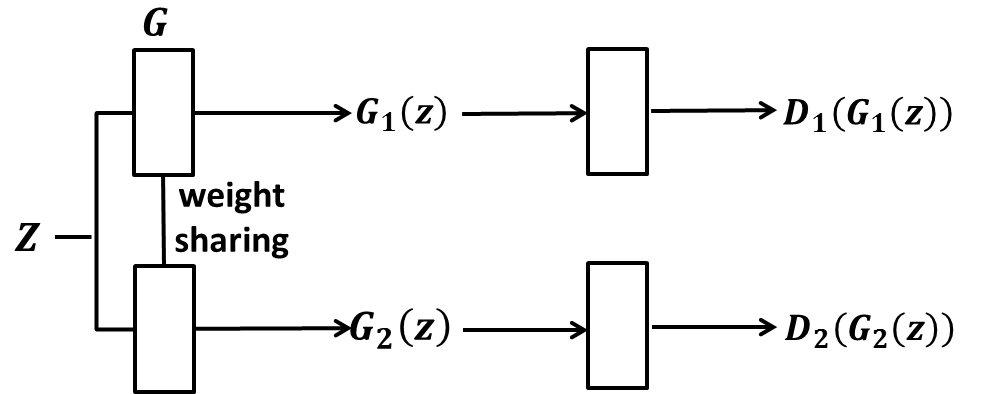
\includegraphics[width=8cm]{images/Coupled_GAN_network.jpg}
                \caption{Coupled GAN网络结构图}
                \label{fig:Coupled GAN网络结构图}
                \end{figure}
            % \textcolor[rgb]{1 0 0}{todo:图片:Coupled GAN网络结构图}
        \subsubsection{CoGAN程序}
            \par
            CoGAN的伪代码如(\ref{code:CoGAN})所示,
            \begin{algorithm}[htbp]
                \caption{Mini-batch stochastic gradient descent for training CoGAN.}\label{code:CoGAN}
                \begin{algorithmic}[1]
                    \State 初始化:网络参数$\theta_{f_1^{(i)}},\theta_{f_2^{(i)}},\theta_{g_1^{(i)}},\theta_{g_s^{(i)}}$;$t,t_{max}$;批量大小$N$。
                    \For {$t=1,2,\dots,t_{max}$}
                        \State 从$p_z$中选取$N$个样本$\{z^1,z^2,\dots,z^N\}$;
                        \State 从$p_{r1}$中选取$N$个样本$\{x_1^1,x_1^2,\dots,x_1^N\}$;
                        \State 从$p_{r2}$中选取$N$个样本$\{x_2^1,x_2^2,\dots,x_2^N\}$;
                        \State 计算判别器$f_1^t$参数的梯度
                        \begin{align*}
                        \nabla_{\theta_{f_1^{(i)}}} \frac{1}{N}\sum_{j=1}^N - \log f_1^t(x_1^j) - \log (1-f_1^t(g_1^t(z^j)))
                        \end{align*}
                        \State 计算判别器$f_2^t$参数的梯度
                        \begin{align*}
                        \nabla_{\theta_{f_2^{(i)}}} \frac{1}{N}\sum_{j=1}^N - \log f_2^t(x_2^j) - \log (1-f_2^t(g_2^t(z^j)))
                        \end{align*}
                        \State 两个判别器之间进行参数平均共享。
                        \State 根据参数的梯度更新判别器$f_1^{t+1}$和$f_2^{t+1}$。
                        \State 计算生成器$g_1^t$参数的梯度
                        \begin{align*}
                        \nabla_{\theta_{g_1^{(i)}}} \frac{1}{N}\sum_{j=1}^N  - \log (1-f_1^{t+1}(g_1^t(z^j)))
                        \end{align*}
                        \State 计算判别器$f_2^t$参数的梯度
                        \begin{align*}
                        \nabla_{\theta_{g_2^{(i)}}} \frac{1}{N}\sum_{j=1}^N - \log (1-f_2^{t+1}(g_2^t(z^j)))
                        \end{align*}
                        \State 两个生成器之间进行参数平均共享。
                        \State 根据参数的梯度更新生成器$g_1^{t+1}$和$g_2^{t+1}$。
                    \EndFor
                \end{algorithmic}
            \end{algorithm}
            \par
            CoGAN的TensorFlow程序如下
            \begin{lstlisting}[language = Python]
            import tensorflow as tf
            from tensorflow.examples.tutorials.mnist import input_data
            import numpy as np
            import matplotlib.pyplot as plt
            import matplotlib.gridspec as gridspec
            import os
            import scipy.ndimage.interpolation
            mnist = input_data.read_data_sets('../../MNIST_data', one_hot=True)
            mb_size = 32
            X_dim = mnist.train.images.shape[1]
            y_dim = mnist.train.labels.shape[1]
            z_dim = 10
            h_dim = 128
            eps = 1e-8
            lr = 1e-3
            d_steps = 3
            def plot(samples):
                fig = plt.figure(figsize=(4, 4))
                gs = gridspec.GridSpec(4, 4)
                gs.update(wspace=0.05, hspace=0.05)
                for i, sample in enumerate(samples):
                    ax = plt.subplot(gs[i])
                    plt.axis('off')
                    ax.set_xticklabels([])
                    ax.set_yticklabels([])
                    ax.set_aspect('equal')
                    plt.imshow(sample.reshape(28, 28), cmap='Greys_r')
                return fig
            def xavier_init(size):
                in_dim = size[0]
                xavier_stddev = 1. / tf.sqrt(in_dim / 2.)
                return tf.random_normal(shape=size, stddev=xavier_stddev)
            X1 = tf.placeholder(tf.float32, shape=[None, X_dim])
            X2 = tf.placeholder(tf.float32, shape=[None, X_dim])
            z = tf.placeholder(tf.float32, shape=[None, z_dim])
            G_W1 = tf.Variable(xavier_init([z_dim, h_dim]))
            G_b1 = tf.Variable(tf.zeros(shape=[h_dim]))
            G1_W2 = tf.Variable(xavier_init([h_dim, X_dim]))
            G1_b2 = tf.Variable(tf.zeros(shape=[X_dim]))
            G2_W2 = tf.Variable(xavier_init([h_dim, X_dim]))
            G2_b2 = tf.Variable(tf.zeros(shape=[X_dim]))
            def G(z):
                h = tf.nn.relu(tf.matmul(z, G_W1) + G_b1)
                G1 = tf.nn.sigmoid(tf.matmul(h, G1_W2) + G1_b2)
                G2 = tf.nn.sigmoid(tf.matmul(h, G2_W2) + G2_b2)
                return G1, G2
            D1_W1 = tf.Variable(xavier_init([X_dim, h_dim]))
            D1_b1 = tf.Variable(tf.zeros(shape=[h_dim]))
            D2_W1 = tf.Variable(xavier_init([X_dim, h_dim]))
            D2_b1 = tf.Variable(tf.zeros(shape=[h_dim]))
            D_W2 = tf.Variable(xavier_init([h_dim, 1]))
            D_b2 = tf.Variable(tf.zeros(shape=[1]))
            def D(X1, X2):
                h1 = tf.nn.relu(tf.matmul(X1, D1_W1) + D1_b1)
                h2 = tf.nn.relu(tf.matmul(X2, D2_W1) + D2_b1)
                D1_out = tf.nn.sigmoid(tf.matmul(h1, D_W2) + D_b2)
                D2_out = tf.nn.sigmoid(tf.matmul(h2, D_W2) + D_b2)
                return D1_out, D2_out
            theta_G = [G1_W2, G2_W2, G1_b2, G2_b2]
            theta_G_shared = [G_W1, G_b1]
            theta_D = [D1_W1, D2_W1, D1_b1, D2_b1]
            theta_D_shared = [D_W2, D_b2]
            # Train D
            G1_sample, G2_sample = G(z)
            D1_real, D2_real = D(X1, X2)
            D1_fake, D2_fake = D(G1_sample, G2_sample)
            D1_loss = -tf.reduce_mean(tf.log(D1_real + eps) + tf.log(1. - D1_fake + eps))
            D2_loss = -tf.reduce_mean(tf.log(D2_real + eps) + tf.log(1. - D2_fake + eps))
            D_loss = D1_loss + D2_loss
            # Train G
            G1_loss = -tf.reduce_mean(tf.log(D1_fake + eps))
            G2_loss = -tf.reduce_mean(tf.log(D2_fake + eps))
            G_loss = G1_loss + G2_loss
            # D optimizer
            D_opt = tf.train.AdamOptimizer(learning_rate=lr)
            # Compute the gradients for a list of variables.
            D_gv = D_opt.compute_gradients(D_loss, theta_D)
            D_shared_gv = D_opt.compute_gradients(D_loss, theta_D_shared)
            # Average by halfing the shared gradients
            D_shared_gv = [(0.5 * x[0], x[1]) for x in D_shared_gv]
            # Update
            D_solver = tf.group(
                D_opt.apply_gradients(D_gv), D_opt.apply_gradients(D_shared_gv)
            )
            # G optimizer
            G_opt = tf.train.AdamOptimizer(learning_rate=lr)
            # Compute the gradients for a list of variables.
            G_gv = G_opt.compute_gradients(G_loss, theta_G)
            G_shared_gv = G_opt.compute_gradients(G_loss, theta_G_shared)
            # Average by halfing the shared gradients
            G_shared_gv = [(0.5 * x[0], x[1]) for x in G_shared_gv]
            # Update
            G_solver = tf.group(
                G_opt.apply_gradients(G_gv), G_opt.apply_gradients(G_shared_gv)
            )
            sess = tf.Session()
            sess.run(tf.global_variables_initializer())
            X_train = mnist.train.images
            half = int(X_train.shape[0] / 2)
            # Real image
            X_train1 = X_train[:half]
            # Rotated image
            X_train2 = X_train[half:].reshape(-1, 28, 28)
            X_train2 = scipy.ndimage.interpolation.rotate(X_train2, 90, axes=(1, 2))
            X_train2 = X_train2.reshape(-1, 28*28)
            # Cleanup
            del X_train
            def sample_X(X, size):
                start_idx = np.random.randint(0, X.shape[0]-size)
                return X[start_idx:start_idx+size]
            def sample_z(m, n):
                return np.random.uniform(-1., 1., size=[m, n])
            if not os.path.exists('out/'):
                os.makedirs('out/')
            i = 0
            for it in range(1000000):
                X1_mb, X2_mb = sample_X(X_train1, mb_size), sample_X(X_train2, mb_size)
                z_mb = sample_z(mb_size, z_dim)
                _, D_loss_curr = sess.run(
                    [D_solver, D_loss],
                    feed_dict={X1: X1_mb, X2: X2_mb, z: z_mb}
                )
                _, G_loss_curr = sess.run(
                    [G_solver, G_loss], feed_dict={z: z_mb}
                )
                if it % 1000 == 0:
                    sample1, sample2 = sess.run(
                        [G1_sample, G2_sample], feed_dict={z: sample_z(8, z_dim)}
                    )
                    samples = np.vstack([sample1, sample2])
                    print('Iter: {}; D_loss: {:.4}; G_loss: {:.4}'
                          .format(it, D_loss_curr, G_loss_curr))
                    fig = plot(samples)
                    plt.savefig('out/{}.png'
                                .format(str(i).zfill(3)), bbox_inches='tight')
                    i += 1
            plt.close(fig)
            \end{lstlisting}

    \subsection{Dual GAN}
        \subsubsection{Dual GAN模型建立}
            \par
            下面,主要考虑条件GAN,因为很多计算机视觉的问题都可以被看成是一种“图片翻译”问题。例如,一张人脸的照片以及与之对应的一张素描之间的相互转换就可以看成是从一张图片“翻译”为另外一张图片(我们可以将素描图片作为生成器$G$的输入的一部分)。事实上,更一般的,边界探测、图像分割、图片的风格化和抽象化等等都可以被视为是这样一种“翻译”问题。
            \par
            而说到“翻译”,很容易会想到其在自然语言处理领域中的一些应用。近年来在机器翻译领域也有许多有意思的新进展。其中一种新的做法是对偶学习(dual learning),这种学习的方式为解决无监督学习中遇到的困难提供了新的思路。简要介绍一下这种学习方法的基本思路:假如现在小明只能讲中文, Alice 只会讲英文,他们两个人虽然都不懂对方的语言,但是他们希望能够可以中英文之间的两个翻译模型(中译英,英译中)。怎样可以实现他们的这个目的呢?首先,对于一个英文的句子,Alice 先用翻译工具将其翻译为中文,由于她并不懂中文,于是她直接把句子发给了小明;但小明又不懂英文,于是小明只能按照中文的语言习惯判断这个句子是否通顺,这可以帮助小明判断这个“英译中”的系统是否做得很好,随后,小明把他修改过的句子再用“中译英”的系统翻译成英文,并把英文句子发给 Alice。Alice 虽然不懂中文,但她能比较经过这一大圈的翻译之后,得到的新句子与最初的版本是否相似。这一信息可以帮助判断是否两个翻译模型都表现良好。随着“对偶学习”过程的持续进行,未标注的数据也得到了充分的利用,利用这些信息,可以帮助提高对偶任务中的两个翻译模型。这种对偶学习的想法为进一步改进现有的翻译模型提出了崭新的思路。如果把这种对偶学习的方法也用到基于GAN的图片的“翻译”上,会得到怎样的效果呢?这会是一个非常有趣的问题。
            \par
            DualGAN 算法就是将基本的 GAN 再进一步扩展为两个相互耦合的的 GAN,其中存在着两个生成器和两个判别器。如图(\ref{fig:DualGAN结构示意图})所示
                \begin{figure}[H]
                \centering
                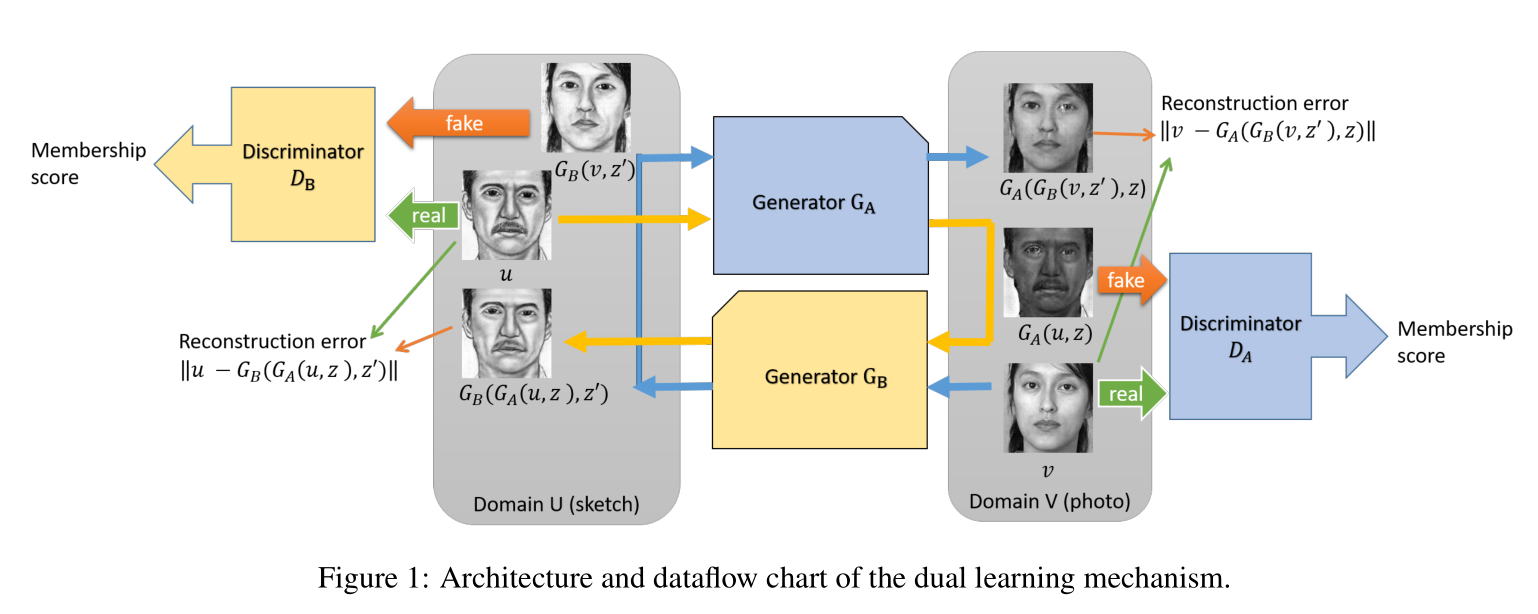
\includegraphics[width=14cm]{images/DualGAN_structure.jpg}
                \caption{DualGAN结构示意图}
                \label{fig:DualGAN结构示意图}
                \end{figure}
            % \textcolor[rgb]{1 0 0}{todo:图片:DualGAN结构示意图}\\
            以素描与照片之间的相互“翻译”为例。设$U$为素描图像集,$V$为照片图像集,原始任务是学习一个生成器$G_A:U\rightarrow V$,$G_A$是从素描$u\sim U$到照片$v\sim V$的映射。与这个生成器对应的有一个判别器 $D_A$,二者构成第一个GAN。与原始任务相对应,存在一个对偶任务:训练一个生成器 $G_B:V\rightarrow U$,将照片转换为素描,与这个生成器所对应的同样有一个判别器 $D_B$,二者形成了第二个GAN(对偶GAN)。
            \par
            在这样的基本框架下,接下来考虑怎样利用对偶学习的思路训练 GAN。首先介绍“生成”的思路,通过生成器$ G_A $可以对素描图片$ u$ 进行翻译,最终得到类似照片的图片,其中包含的噪声为$ z$,翻译的结果即为 $G_A(u,z)$ ,把这个翻译的结果扔给另一个专门用于生成素描图片的生成器$ G_B$,得到的结果$ G_B(G_A(u, z),z') $即为对原有的素描图片的一次重构,这里的$ z'$ 同样是噪声。接下来考虑与这一过程对偶的一个过程,首先将照片$ v $用生成器$ G_B$翻译为素描图$ G_B(v,z') $,然后再用生成器$ G_A $对生成的素描图进行翻译,得到 $G_A(G_B(v,z'),z)$ 。接下来介绍“判别”的思路,与生成器$ G_A $对应的判别器$ D_A $判断一张图片是否像一张照片,而与生成器$ G_B $对应的判别器$ D_B $则判断一张图片是否像一张素描图。对应于上面提到的对偶的生成过程,系统最终希望最小化重构误差,即希望最小化在两次迭代后得到的结果与原始图片之间的误差$|| G_A(G_B(v,z'),z)-v || $和$|| G_B(G_A(u,z),z')-u || $。
            \par
            像传统GAN训练判别器D那样,在DualGAN中,判别器D的目标仍然是将真假样本区分开。由于WGAN在许多方面优于GAN,DualGAN采用WGAN作为GAN的替代,相应的判别器$D_A$和$D_B$的损失函数定义为
            \begin{align*}
            l_A^d(u,v) = D_A(G_A(u,z)) - D_A(v)\\
            l_B^d(u,v) = D_B(G_B(v,z')) - D_B(u)
            \end{align*}
            其中:$u\sim U,v\sim V$。
            \par
            对于生成器$G$而言,$G_A$和$G_B$有共同的目标,因此二者使用同一损失函数。之前的条件图像合成方法发现,使用$L1$距离替代$L2$距离是较好的,因为$L2$经常导致图像模糊。因此,我们使用$L1$距离来衡量重构误差,添加到GAN生成器G的目标中,有
            \begin{align*}
            l^g(u,v) &= \lambda_U||u-G_B(G_A(u,z),z')||+\lambda_V||v-G_A(G_B(v,z'),z)||\\
            &\quad -D_A(G_B(v,z')) - D_B(G_A(u,z))
            \end{align*}
            其中:$u\sim U,v\sim V$,$\lambda_U,\lambda_V$是两个惩罚权重。合适的$\lambda_U,\lambda_V$是$100\sim 1000$,并且,如果$U$是自然图片而$V$不是,那么将$\lambda_U$设置的比$\lambda_V$小是有用的。
        \subsubsection{Dual GAN程序及代码}
            \par
            上面我们提到过,在DualGAN中使用WGAN来替代GAN。下面,给出DualGAN中的一些设置。我们训练$n_{critic}$步判别器$D$,然后训练1步$G$;使用mini-batch的批量梯度下降方法求解模型中的优化问题,并使用RMSProp作为求解器(Adam等基于动量的方法可能导致训练不稳定);$n_{critic}$一般设置为$2\sim 4$,批量大小一般为$1\sim 4$,权重修剪(wight clipping)参数$c$一般设置在$0.01\sim 0.1$。DualGAN的算法伪代码如(\ref{code:DualGAN})所示
            \begin{algorithm}[H]
                \caption{DualGAN training procedure}\label{code:DualGAN}
                \begin{algorithmic}[1]
                    \State 初始化:图像数据集$U$和$V$;GAN $A$的生成器参数为$\theta_A$,判别器参数为 $\omega_A$;GAN $B$的生成器参数为$\theta_B$,判别器参数为 $\omega_B$;修剪参数$c$;批量大小$m$;循环$n_{critic}$。
                    \State 随机初始化$\omega_i,\theta_i$,$i\in \{A,B\}$。
                    \While {未达到停止准则}
                        \For {$t=1$ to $n_{critic}$}
                            \State 采样$\{u^{(k)}\}_{k=1}^m\sim U$,$\{v^{(k)}\}_{k=1}^m\sim V$;
                            \State 更新参数$\omega_A$
                            \begin{align*}
                            \frac{1}{m} \sum_{k=1}^m l_A^d ( u^{(k)},v^{(k)} )
                            \end{align*}
                            \State 更新参数$\omega_B$
                            \begin{align*}
                            \frac{1}{m} \sum_{k=1}^m l_B^d ( u^{(k)},v^{(k)} )
                            \end{align*}
                            \State $clip(\omega_A,-c,c)$,$clip(\omega_B,-c,c)$;
                        \EndFor
                        \State 采样$\{u^{(k)}\}_{k=1}^m\sim U$,$\{v^{(k)}\}_{k=1}^m\sim V$;
                        \State 更新$\theta_A,\theta_B$
                        \begin{align*}
                        \frac{1}{m} \sum_{k=1}^m l^g ( u^{(k)},v^{(k)} )
                        \end{align*}
                    \EndWhile
                \end{algorithmic}
            \end{algorithm}
            \par
            DualGAN的TensorFlow代码如下
            \begin{lstlisting}[language = Python]
            import tensorflow as tf
            from tensorflow.examples.tutorials.mnist import input_data
            import numpy as np
            import matplotlib.pyplot as plt
            import matplotlib.gridspec as gridspec
            import os
            import scipy.ndimage.interpolation
            mnist = input_data.read_data_sets('../../MNIST_data', one_hot=True)
            mb_size = 32
            X_dim = mnist.train.images.shape[1]
            y_dim = mnist.train.labels.shape[1]
            z_dim = 10
            h_dim = 128
            eps = 1e-8
            lr = 1e-3
            d_steps = 3
            lam1, lam2 = 1000, 1000
            def plot(samples):
                fig = plt.figure(figsize=(4, 4))
                gs = gridspec.GridSpec(4, 4)
                gs.update(wspace=0.05, hspace=0.05)
                for i, sample in enumerate(samples):
                    ax = plt.subplot(gs[i])
                    plt.axis('off')
                    ax.set_xticklabels([])
                    ax.set_yticklabels([])
                    ax.set_aspect('equal')
                    plt.imshow(sample.reshape(28, 28), cmap='Greys_r')
                return fig
            def xavier_init(size):
                in_dim = size[0]
                xavier_stddev = 1. / tf.sqrt(in_dim / 2.)
                return tf.random_normal(shape=size, stddev=xavier_stddev)
            X1 = tf.placeholder(tf.float32, shape=[None, X_dim])
            X2 = tf.placeholder(tf.float32, shape=[None, X_dim])
            z = tf.placeholder(tf.float32, shape=[None, z_dim])
            G1_W1 = tf.Variable(xavier_init([X_dim + z_dim, h_dim]))
            G1_b1 = tf.Variable(tf.zeros(shape=[h_dim]))
            G1_W2 = tf.Variable(xavier_init([h_dim, X_dim]))
            G1_b2 = tf.Variable(tf.zeros(shape=[X_dim]))
            G2_W1 = tf.Variable(xavier_init([X_dim + z_dim, h_dim]))
            G2_b1 = tf.Variable(tf.zeros(shape=[h_dim]))
            G2_W2 = tf.Variable(xavier_init([h_dim, X_dim]))
            G2_b2 = tf.Variable(tf.zeros(shape=[X_dim]))
            def G1(X1, z):
                inputs = tf.concat([X1, z], 1)
                h = tf.nn.relu(tf.matmul(inputs, G1_W1) + G1_b1)
                return tf.nn.sigmoid(tf.matmul(h, G1_W2) + G1_b2)
            def G2(X2, z):
                inputs = tf.concat([X2, z], 1)
                h = tf.nn.relu(tf.matmul(inputs, G2_W1) + G2_b1)
                return tf.nn.sigmoid(tf.matmul(h, G2_W2) + G2_b2)
            D1_W1 = tf.Variable(xavier_init([X_dim, h_dim]))
            D1_b1 = tf.Variable(tf.zeros(shape=[h_dim]))
            D1_W2 = tf.Variable(xavier_init([h_dim, 1]))
            D1_b2 = tf.Variable(tf.zeros(shape=[1]))
            D2_W1 = tf.Variable(xavier_init([X_dim, h_dim]))
            D2_b1 = tf.Variable(tf.zeros(shape=[h_dim]))
            D2_W2 = tf.Variable(xavier_init([h_dim, 1]))
            D2_b2 = tf.Variable(tf.zeros(shape=[1]))
            def D1(X):
                h = tf.nn.relu(tf.matmul(X, D1_W1) + D1_b1)
                return tf.matmul(h, D1_W2) + D1_b2
            def D2(X):
                h = tf.nn.relu(tf.matmul(X, D1_W1) + D1_b1)
                return tf.matmul(h, D2_W2) + D2_b2
            theta_G1 = [G1_W1, G1_W2, G1_b2, G1_b2]
            theta_G2 = [G2_W1, G2_b1, G2_W2, G2_b2]
            theta_G = theta_G1 + theta_G2
            theta_D1 = [D1_W1, D1_W2, D1_b1, D1_b2]
            theta_D2 = [D2_W1, D2_b1, D2_W2, D2_b2]
            # D
            X1_sample = G2(X2, z)
            X2_sample = G1(X1, z)
            D1_real = D1(X2)
            D1_fake = D1(X2_sample)
            D2_real = D2(X1)
            D2_fake = D2(X1_sample)
            D1_G = D1(X1_sample)
            D2_G = D2(X2_sample)
            X1_recon = G2(X2_sample, z)
            X2_recon = G1(X1_sample, z)
            recon1 = tf.reduce_mean(tf.reduce_sum(tf.abs(X1 - X1_recon), 1))
            recon2 = tf.reduce_mean(tf.reduce_sum(tf.abs(X2 - X2_recon), 1))
            D1_loss = tf.reduce_mean(D1_fake) - tf.reduce_mean(D1_real)
            D2_loss = tf.reduce_mean(D2_fake) - tf.reduce_mean(D2_real)
            G_loss = -tf.reduce_mean(D1_G + D2_G) + lam1*recon1 + lam2*recon2
            D1_solver = (tf.train.RMSPropOptimizer(learning_rate=1e-4)
                         .minimize(D1_loss, var_list=theta_D1))
            D2_solver = (tf.train.RMSPropOptimizer(learning_rate=1e-4)
                         .minimize(D2_loss, var_list=theta_D2))
            G_solver = (tf.train.RMSPropOptimizer(learning_rate=1e-4)
                        .minimize(G_loss, var_list=theta_G))
            clip_D = [p.assign(tf.clip_by_value(p, -0.01, 0.01)) for p in theta_D1 + theta_D2]
            sess = tf.Session()
            sess.run(tf.global_variables_initializer())
            X_train = mnist.train.images
            half = int(X_train.shape[0] / 2)
            # Real image
            X_train1 = X_train[:half]
            # Rotated image
            X_train2 = X_train[half:].reshape(-1, 28, 28)
            X_train2 = scipy.ndimage.interpolation.rotate(X_train2, 90, axes=(1, 2))
            X_train2 = X_train2.reshape(-1, 28*28)
            # Cleanup
            del X_train
            def sample_X(X, size):
                start_idx = np.random.randint(0, X.shape[0]-size)
                return X[start_idx:start_idx+size]
            def sample_z(m, n):
                return np.random.uniform(-1., 1., size=[m, n])
            if not os.path.exists('out/'):
                os.makedirs('out/')
            i = 0
            for it in range(1000000):
                for _ in range(d_steps):
                    X1_mb, X2_mb = sample_X(X_train1, mb_size), sample_X(X_train2, mb_size)
                    z_mb = sample_z(mb_size, z_dim)
                    _, _, D1_loss_curr, D2_loss_curr, _ = sess.run(
                        [D1_solver, D2_solver, D1_loss, D2_loss, clip_D],
                        feed_dict={X1: X1_mb, X2: X2_mb, z: z_mb}
                    )
                _, G_loss_curr = sess.run(
                    [G_solver, G_loss], feed_dict={X1: X1_mb, X2: X2_mb, z: z_mb}
                )
                if it % 1000 == 0:
                    sample1, sample2 = sess.run(
                        [X1_sample, X2_sample],
                        feed_dict={X1: X1_mb[:4], X2: X2_mb[:4], z: sample_z(4, z_dim)}
                    )
                    samples = np.vstack([X1_mb[:4], sample1, X2_mb[:4], sample2])
                    print('Iter: {}; D_loss: {:.4}; G_loss: {:.4}'
                          .format(it, D1_loss_curr + D2_loss_curr, G_loss_curr))
                    fig = plot(samples)
                    plt.savefig('out/{}.png'
                                .format(str(i).zfill(3)), bbox_inches='tight')
                    i += 1
            plt.close(fig)
            \end{lstlisting}
        \subsubsection{Dual GAN实验结果}
            \par
            根据这一基本思路,就可以真的来对图片做各种处理了。下面了展示这一算法得到的一些结果。这些相关结果分别与真实情况(ground truth)和其它算法得到的结果进行了比较,可以发现这一算法的确有着不错的表现。
            将DualGAN和GAN、CGAN在图片翻译数据集上进行比较。日景图片与夜景图片之间的转换结果如图(\ref{fig:DualGAN日景图片与夜景图片之间的转换})所示
                \begin{figure}[H]
                \centering
                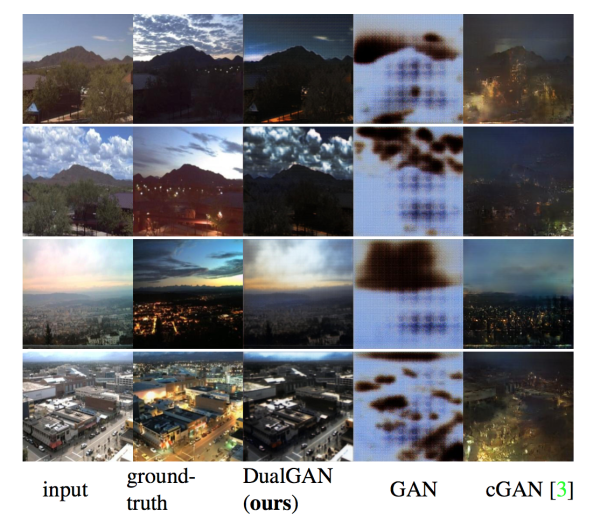
\includegraphics[width=8cm]{images/DualGAN.jpg}
                \caption{DualGAN日景图片与夜景图片之间的转换}
                \label{fig:DualGAN日景图片与夜景图片之间的转换}
                \end{figure}
            % \textcolor[rgb]{1 0 0}{todo:图片:DualGAN日景图片与夜景图片之间的转换}\\
            素描与照片之间的相互翻译结果如图(\ref{fig:DualGAN素描与照片之间的相互翻译})所示
            \begin{figure}[H]
            \centering
            \begin{subfigure}[b]{0.4\textwidth}
            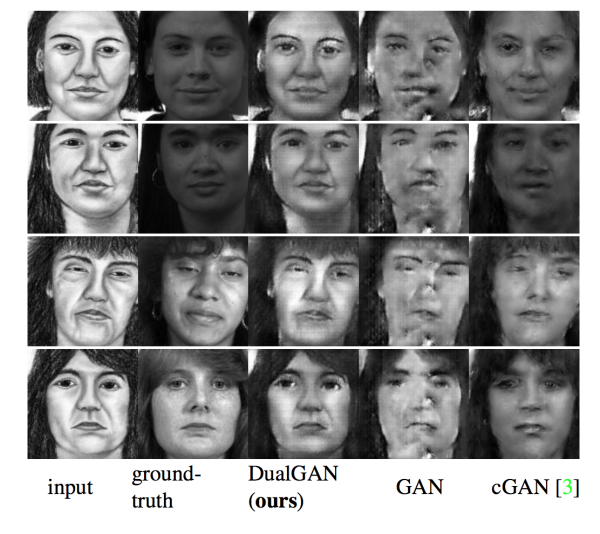
\includegraphics[width=\textwidth]{images/DualGAN_picture_translation1.jpg}
            \caption{}
            \end{subfigure}
            \begin{subfigure}[b]{0.4\textwidth}
            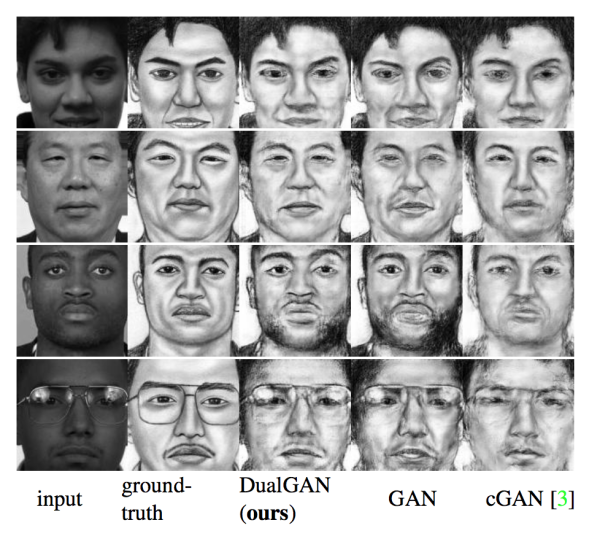
\includegraphics[width=\textwidth]{images/DualGAN_picture_translation2.jpg}
            \caption{}
            \end{subfigure}
            \caption{DualGAN素描与照片之间的相互翻译}
            \label{fig:DualGAN素描与照片之间的相互翻译}
            \end{figure}
            % \textcolor[rgb]{1 0 0}{todo:图片:DualGAN素描与照片之间的相互翻译(b)}

    \subsection{Boundary Equilibrium GAN}
        \subsubsection{BEGAN模型建立}
            \par
            注:GAN以生成器G为主,D为辅,可以设计以D为主,以G为辅的网络结构。
            BEGAN\cite{2017.David}使用一个自动编码器作为判别器(在EBGAN\cite{2016.Junbo}中首先提出)。典型的GAN想要直接匹配数据分布,而BEGAN的目标是用一个来自Wassers tein距离的损失来匹配自动编码器的损失分布。这一目标是通过在典型GAN的目标中添加一个equilibeium部分实现的。equilibeium部分用于平衡D和G,和GAN相比,BEGAN有更简单的训练程序和网络结构。
            \paragraph{自动编码器的Wasserstein距离}我们希望学习残差分布而不是直接学习样本分布。首先说明一个自动编码器的损失近似一个 normal distribution,然后计算真实样本和生成样本的自动编码器的损失分布的Wassertein距离。定义$\mathcal{L}:R^{N_x}\to R$是像素自动编码器的损失
            \begin{align*}
            \mathcal{L}(v) =|v-D(v)|^\eta
            \end{align*}
            其中:$D:R^{N_x}\to R^{N_x}$是自动编码器,$\eta\in \{1,2\}$,$v\in  R^{N_x}$是一个维度为$N_x$的样本。对于足够多的像素点,如果假设各像素点的loss是独立同分布的,根据中心极限定理,图像的损失分布服从一个近似正太分布。在BEGAN中,我们使用原始图像和重建后图像的$L_1$范数作为loss。在实验中作者发现,在实验数据上,loss distribution 真的接近正态。
            \par
            给定两个正态分布$\mu_1 = N(m_1,C_1),\mu_2 = N(m_2,C_2)$,其均值为$m_1,m_2\in R^p$,协方差矩阵为$C_1,C_2\in R^{p\times p}$,二者的平方Wasserstein距离定义为
            \begin{align*}
            W(\mu_1,\mu_2)^2 = ||m_1-m_2||_2^2 + \mathrm{Tr}(C_1+C_2-2(C_2^{1/2}C_1C_2^{1/2})^{1/2})
            \end{align*}
            特别地,当$p=1$时,平方Wsaaerstein距离简化为
            \begin{align*}
            W(\mu_1,\mu_2)^2 = ||m_1-m_2||_2^2 +(c_1+c_2-2\sqrt{c_1c_2})
            \end{align*}
            \par
            我们希望在实验中优化$W^2$时,只需要优化$||m_1-m_2||_2^2$即可,而当$\frac{c_1+c_2-2\sqrt{c_1c_2}}{||m_1-m_2||_2^2}$是常数或者单调增时,真的就只需要优化$||m_1-m_2||_2^2$。这使得我们可以将目标简化为
            \begin{align*}
            W(\mu_1,\mu_2)^2 \propto ||m_1-m_2||_2^2
            \end{align*}
            值得一提的是,我们是准备优化loss分布的$W^2$距离,而不是样本分布。设定训练误差分布比训练样本分布更稳定。
            \paragraph{GAN的目标}我们求$D$来最大化$W^2 \propto ||m_1-m_2||_2^2$。设$\mu_1$是损失$\mathcal{L}(x)$的分布,这里的$x$是真实样本;设$\mu_2$是损失$\mathcal{L}(G(z))$的分布,这里$G:R^{N_x}\to R^{N_x}$是一个生成器,$z\in [-1,1]^{N_z}$是$N_z$维的随机量。
            \par
            由于$m_1,m_2\in R^+$,所以$W^2$只有2种可能
            \begin{align*}
            (a)\left\{
            \begin{aligned}
            &W(\mu_1,\mu_2) \propto m_1-m_2\\
            &m_1\to \infty\\
            &m_2\to 0
            \end{aligned}
            \right.
            \quad
            or
            \quad
            (b)\left\{
            \begin{aligned}
            &W(\mu_1,\mu_2) \propto m_2-m_1\\
            &m_1\to 0\\
            &m_2\to \infty
            \end{aligned}
            \right.
            \end{align*}
            我们按照目标选择(b)这种情况,因为最小的$m_1$自然地自动编码真实图像。设D和G的参数分别为$\theta_d,\theta_g$,通过最小化D和G的损失$\mathcal{L}_D,\mathcal{L}_G$来求解参数
            \begin{align*}
            & \mathcal{L}_D = \mathcal{L}(x;\theta_d) - \mathcal{L}(G(z_D;\theta_g);\theta_g)\\
            & \mathcal{L}_G = \mathcal{L}(G(z_G;\theta_g);\theta_d)
            \end{align*}
            其中:$z_G,z_D$是来自$z$的样本。下面,将$G(\cdot,\theta_g)$简记为$G(\cdot)$,将$L(\cdot,\theta_d)$简记为$L(\cdot)$。
            \par
            和WGAN相比,上面的目标主要有两方面的不同:\ding{172}BEGAN是在假设的正态损失间构建分布;\ding{173}BEGAN不需要k-lipschitz假设。
            \paragraph{Equilibrium}在实践中,保持D和G的平衡是至关重要的,当
            \begin{align*}
            \mathbb{E}[\mathcal{L}(x)] = \mathbb{E}[\mathcal{L}(G(z))]
            \end{align*}
            时,我们认为二者是平衡的。如果我们生成的样本不能被D辨识真假,那么真假样本的误差分布应该相同。这个观点允许我们通过分配G和D来平衡the effect,因此,不存在赢的一方。
            \par
            当存在完美的平衡时,如果$m_1-m_2\to 0$,则$\frac{c_1+c_2-2\sqrt{c_1c_2}}{||m_1-m_2||_2^2}$变得不稳定。通过引入一个超参数$\gamma\in [0,1]$来解决这个问题
            \begin{align*}
            \gamma = \frac{\mathbb{E}[\mathcal{L}(G(z))]}{\mathbb{E}[\mathcal{L}(x)] }
            \end{align*}
            \par
            在我们的模型中,D有两个主要的目标:\ding{172}自动编码真实图像;\ding{173}判别真实图像判别真实图像。$\gamma$部分能够平衡这两个目标,较小的$\gamma$导致低的图像多样性(diversity),因为D集中更多的力量去编码真实图像。我们称$\gamma$为 diversity ratio。
            \paragraph{Boundary Equilibrium GAN}BEGAN的目标是
            \begin{align*}
            & \mathcal{L}_D = \mathcal{L}(x) - k_t\mathcal{L}(G(z_D))\quad& \theta_d\\
            & \mathcal{L}_G = \mathcal{L}(G(z_G))\quad& \theta_g\\
            & k_{t+1} = k_t + \lambda_k(\gamma\mathcal{L}(x)-\mathcal{L}(G(z_G))) \quad& \text{for each training step t}
            \end{align*}
            我们使用比例控制定理( Proportional Control Theory)来保持等式$\mathbb{E}[\mathcal{L}(G(z))]=\gamma \mathbb{E}[\mathcal{L}(x)]$。这里通过变量$k_t\in [0,1]$来决定在梯度下降时,将多少“注意力”放在$\mathcal{L}(G(z_D))$。
            \par
            初始化$k_0 = 0$,$\lambda_k$随着$k$的增加而增加。在主要的学习部分,$\lambda_k$是基于$k$的学习率。本质上,这种平衡可以被视为一个闭环反馈控制形式,其中,在每一步调整$k_t$以维持方程$\gamma = \frac{\mathbb{E}[\mathcal{L}(G(z))]}{\mathbb{E}[\mathcal{L}(x)]}$。
            \par
            在早期的训练过程中,G趋于产生易于自动编码器重建的数据,因为生成数据接近于0,真实数据分布还没有被准确的学习。在整个训练过程中$\mathcal{L}(x) > \mathcal{L}(G(z))$是由平衡约束来实现的。和传统的交替优化G和D的GAN相比, 我们提出的方法在训练时不需要稳定。在训练时使用Adam方法,并设置批量大小为16。
            \par
            通过Equilibrium的概念,我们获得了一个度量收敛性的全局量,可以设计收敛过程是寻找带$|\gamma\mathcal{L}(x)-\mathcal{L}(G(z_G))|$的 closest reconstruction $\mathcal{L}(x)$,表示为
            \begin{align*}
            \mathcal{M}_{global} = \mathcal{L}(x)+ |\gamma\mathcal{L}(x)-\mathcal{L}(G(z_G))|
            \end{align*}
            这个收敛性度量$\mathcal{M}_{global}$可以用于确定网络什么时候达到最终状态,或者判定模型是否崩溃。

        \subsubsection{BEGAN模型程序}
            \par
            BEGAN的TensorFlow程序如下
            \begin{lstlisting}[language = Python]
            import tensorflow as tf
            from tensorflow.examples.tutorials.mnist import input_data
            import numpy as np
            import matplotlib.pyplot as plt
            import matplotlib.gridspec as gridspec
            import os
            mb_size = 32
            X_dim = 784
            z_dim = 64
            h_dim = 128
            lr = 1e-3
            m = 5
            lam = 1e-3
            gamma = 0.5
            k_curr = 0
            mnist = input_data.read_data_sets('../../MNIST_data', one_hot=True)
            def plot(samples):
                fig = plt.figure(figsize=(4, 4))
                gs = gridspec.GridSpec(4, 4)
                gs.update(wspace=0.05, hspace=0.05)
                for i, sample in enumerate(samples):
                    ax = plt.subplot(gs[i])
                    plt.axis('off')
                    ax.set_xticklabels([])
                    ax.set_yticklabels([])
                    ax.set_aspect('equal')
                    plt.imshow(sample.reshape(28, 28), cmap='Greys_r')
                return fig
            def xavier_init(size):
                in_dim = size[0]
                xavier_stddev = 1. / tf.sqrt(in_dim / 2.)
                return tf.random_normal(shape=size, stddev=xavier_stddev)
            X = tf.placeholder(tf.float32, shape=[None, X_dim])
            z = tf.placeholder(tf.float32, shape=[None, z_dim])
            k = tf.placeholder(tf.float32)
            D_W1 = tf.Variable(xavier_init([X_dim, h_dim]))
            D_b1 = tf.Variable(tf.zeros(shape=[h_dim]))
            D_W2 = tf.Variable(xavier_init([h_dim, X_dim]))
            D_b2 = tf.Variable(tf.zeros(shape=[X_dim]))
            G_W1 = tf.Variable(xavier_init([z_dim, h_dim]))
            G_b1 = tf.Variable(tf.zeros(shape=[h_dim]))
            G_W2 = tf.Variable(xavier_init([h_dim, X_dim]))
            G_b2 = tf.Variable(tf.zeros(shape=[X_dim]))
            theta_G = [G_W1, G_W2, G_b1, G_b2]
            theta_D = [D_W1, D_W2, D_b1, D_b2]
            def sample_z(m, n):
                return np.random.uniform(-1., 1., size=[m, n])
            def G(z):
                G_h1 = tf.nn.relu(tf.matmul(z, G_W1) + G_b1)
                G_log_prob = tf.matmul(G_h1, G_W2) + G_b2
                G_prob = tf.nn.sigmoid(G_log_prob)
                return G_prob
            def D(X):
                D_h1 = tf.nn.relu(tf.matmul(X, D_W1) + D_b1)
                X_recon = tf.matmul(D_h1, D_W2) + D_b2
                return tf.reduce_mean(tf.reduce_sum((X - X_recon)**2, 1))
            G_sample = G(z)
            D_real = D(X)
            D_fake = D(G_sample)
            D_loss = D_real - k*D_fake
            G_loss = D_fake
            D_solver = (tf.train.AdamOptimizer(learning_rate=lr)
                        .minimize(D_loss, var_list=theta_D))
            G_solver = (tf.train.AdamOptimizer(learning_rate=lr)
                        .minimize(G_loss, var_list=theta_G))
            sess = tf.Session()
            sess.run(tf.global_variables_initializer())
            if not os.path.exists('out/'):
                os.makedirs('out/')
            i = 0
            for it in range(1000000):
                X_mb, _ = mnist.train.next_batch(mb_size)
                _, D_real_curr = sess.run(
                    [D_solver, D_real],
                    feed_dict={X: X_mb, z: sample_z(mb_size, z_dim), k: k_curr}
                )
                _, D_fake_curr = sess.run(
                    [G_solver, D_fake],
                    feed_dict={X: X_mb, z: sample_z(mb_size, z_dim)}
                )
                k_curr = k_curr + lam * (gamma*D_real_curr - D_fake_curr)
                if it % 1000 == 0:
                    measure = D_real_curr + np.abs(gamma*D_real_curr - D_fake_curr)
                    print('Iter-{}; Convergence measure: {:.4}'
                          .format(it, measure))
                    samples = sess.run(G_sample, feed_dict={z: sample_z(16, z_dim)})
                    fig = plot(samples)
                    plt.savefig('out/{}.png'
                                .format(str(i).zfill(3)), bbox_inches='tight')
                    i += 1
            plt.close(fig)
            \end{lstlisting}
        \subsubsection{BEGAN实验}
            \par
            关于BEGAN模型更详细的网络设置可以参考BEGAN原文,也可以参考上面的BEGAN程序。下面,介绍一些BEGAN的实验结果。
            \paragraph{图像多样性和质量}作者将BEGAN和EBGAN进行了对比,图(\ref{fig:BEGAN的Figure2})给出了一些具有代表性的生成图像
                \begin{figure}[H]
                \centering
                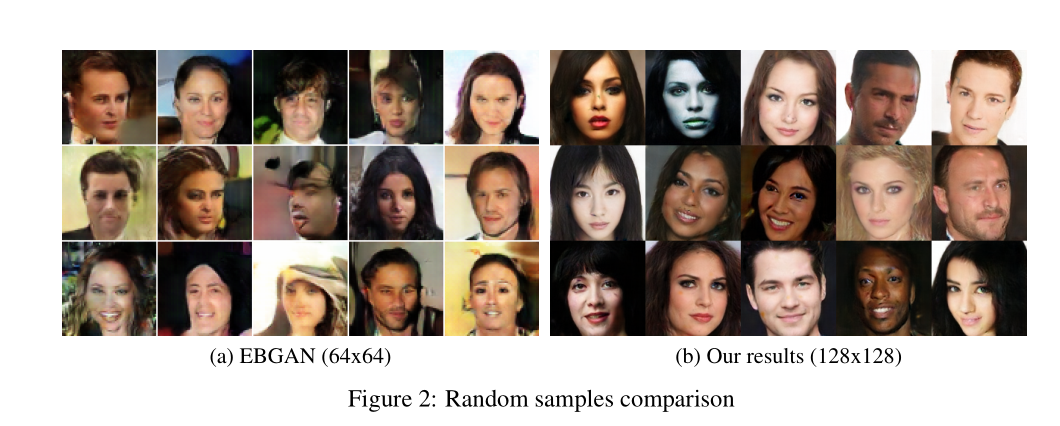
\includegraphics[width=8cm]{images/BEGAN_Figure2.jpg}
                \caption{BEGAN的Figure2}
                \label{fig:BEGAN的Figure2}
                \end{figure}
            % \textcolor[rgb]{1 0 0}{todo:图片:BEGAN的Figure2}\\
            图像大小(分辨率)为$128\times 128$。尽管像常见的那样:训练高分辨率的图像会使图像的清晰度下降,但这也许可以通过超参数来进行调节。这可能是目前为止Stack GAN之外,第2好的分辨率结果。Stack GAN在花和鸟数据集上有$256\times 256$的分辨率。
            \par
            我们可以从生成的图像中看到不同的姿态、表情、性别、肤色、光照和面部毛发等,然而并没有眼睛。但是,值得一提的是,由于BEGAN和EBGAN在不同的训练集上进行训练,因此一般不对他们进行直接比较。
            \par
            在图(\ref{fig:BEGAN的Figure3})中,我们比较了不同参数$\gamma$带来的效果。当$\gamma$在一定范围内时,模型表现出很好的性能,仍然保持一定的图像多样性。当$\gamma$较小时,生成的脸看起来相似,随着$\gamma$的增加,图像多样性增加。这似乎与其它文献中“多样性与图像质量无关”的论断相矛盾。
                \begin{figure}[H]
                \centering
                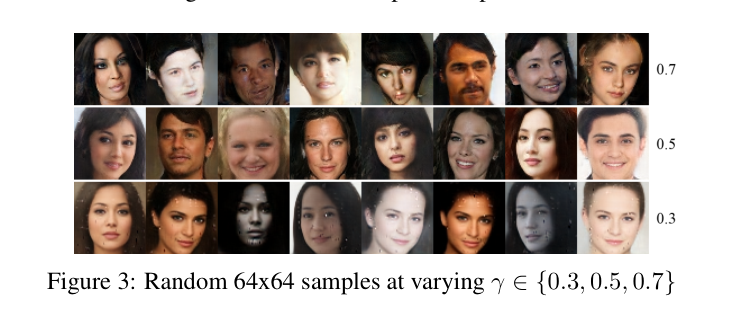
\includegraphics[width=8cm]{images/BEGAN_Figure3.jpg}
                \caption{BEGAN的Figure3}
                \label{fig:BEGAN的Figure3}
                \end{figure}
            % \textcolor[rgb]{1 0 0}{todo:图片:BEGAN的Figure3}
            \paragraph{Space continuity} 为了估计(评价)BEGAN中G的收敛性,我们使真实图像$x_r$和生成$G(z_r)$相一致。用Adam来做,就是找一个$z_r$,最小化$e_r = |x_r - G(z_r)|$。求真实数据的映射并不是模型的目标,但是它提供一个测量生成器G生成能力的方法。通过将$z_r$埋藏在两个真实图像中,我们验证,该模型会概括图像的内容而不是简单的记住图像。
            \par
            图(\ref{fig:BEGAN的Figure4})显示$z_r$在$128\times 128$的分辨率之间的插值。这些图像并不是训练数据的一部分。第一列和最后一列是需要表示和插值的真实图像,紧邻它们的图像是它们相应的近似值,而两列之间的其他图像是线性插值的结果。我们将结果和其它模型进行比较,选用ALI插值的$64\times 64$分辨率和Pixel GNN插值的$32\times 32$分辨率作为比较对象,对不同的数据集进行训练。此外,图(\ref{fig:BEGAN的Figure4})d展示了图像和其镜像的插值结果。
                \begin{figure}[H]
                \centering
                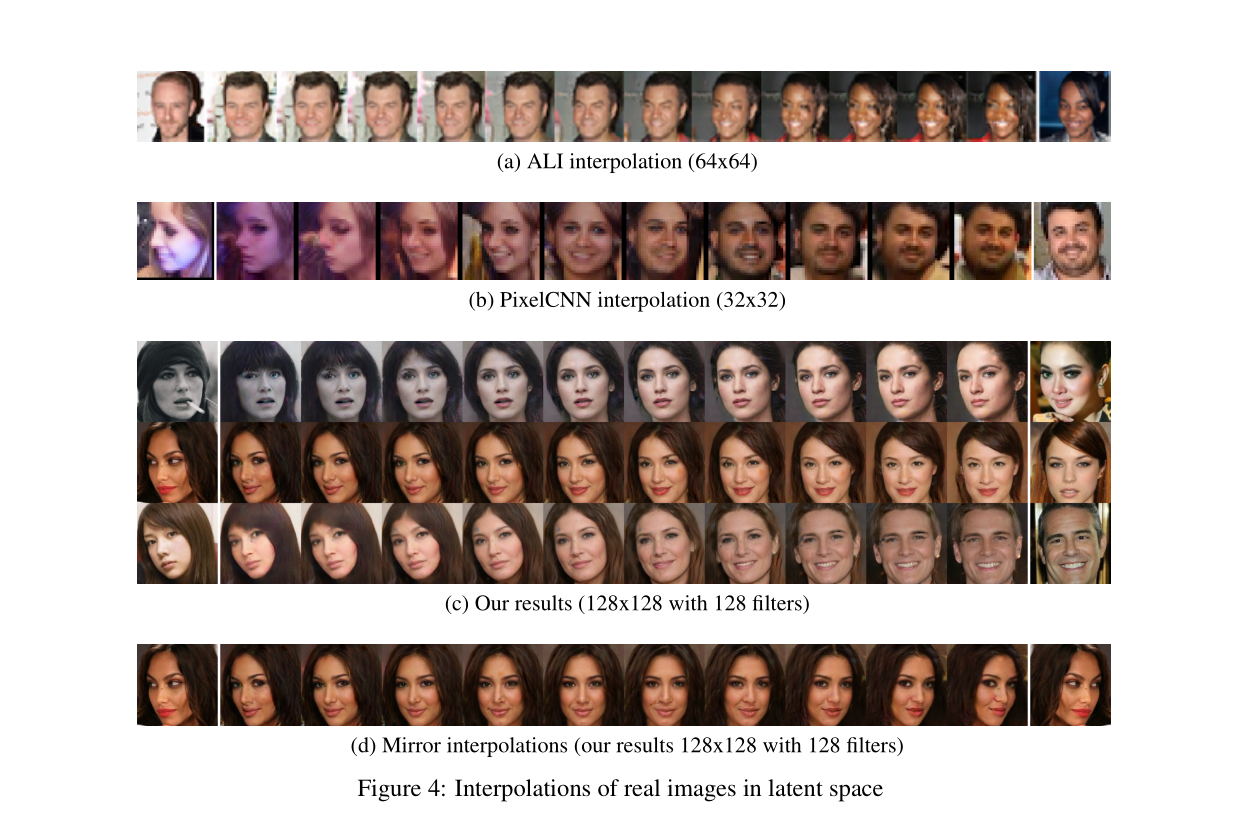
\includegraphics[width=12cm]{images/BEGAN_Figure4.jpg}
                \caption{BEGAN的Figure4}
                \label{fig:BEGAN的Figure4}
                \end{figure}
            % \textcolor[rgb]{1 0 0}{todo:图片:BEGAN的Figure4}
            \paragraph{收敛性度量和图像质量}收敛性度量$\mathcal{M}_{global}$用于度量BEGAN的收敛性,像在图(\ref{fig:BEGAN的Figure5})中看到的那样,$\mathcal{M}_{global}$度量和图像精度(fidelity)有很高的相关性。我们也可以从plot中看出,模型收敛性是较快的,这似乎证明了,快速收敛会导致像素损失。
                \begin{figure}[H]
                \centering
                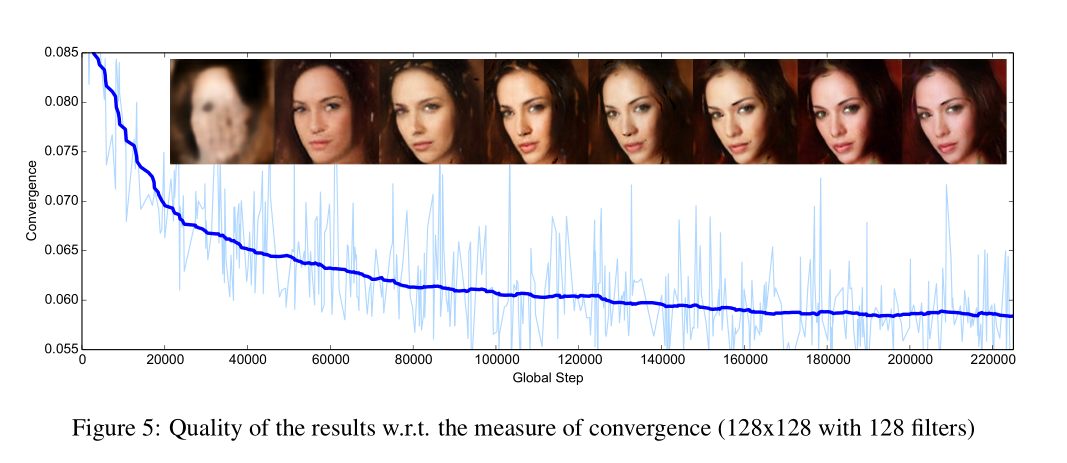
\includegraphics[width=10cm]{images/BEGAN_Figure5.jpg}
                \caption{BEGAN的Figure5}
                \label{fig:BEGAN的Figure5}
                \end{figure}
            % \textcolor[rgb]{1 0 0}{todo:图片:BEGAN的Figure5}
            \paragraph{Equilibrium for unbalanced networks}为了测试平衡技术的鲁棒性,作者进行了一个实验,图(\ref{fig:BEGAN的Figure6})展示了这个结果。令人吃惊的是,低纬度的$h$对图像多样性和图像质量的影响不大。
                \begin{figure}[H]
                \centering
                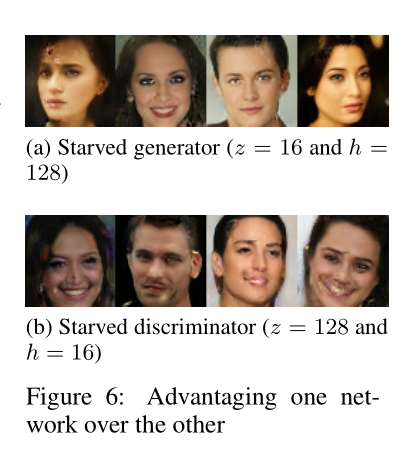
\includegraphics[width=6cm]{images/BEGAN_Figure6.jpg}
                \caption{BEGAN的Figure6}
                \label{fig:BEGAN的Figure6}
                \end{figure}


    % \subsection{Generative Adversarial Parallelization}
    % \subsection{Auxiliary Classifier GAN}
    % \subsection{Energy Based GAN}
    % \subsection{DiscoGAN}


% \bibliography{part-MLDL-chap-DeepLearn}%bib文件名称
% \end{document}
